\documentclass[a4paper]{book}
\usepackage{makeidx}
\usepackage{graphicx}
\usepackage{multicol}
\usepackage{float}
\usepackage{listings}
\usepackage{color}
\usepackage{ifthen}
\usepackage[table]{xcolor}
\usepackage{textcomp}
\usepackage{alltt}
\usepackage{ifpdf}
\ifpdf
\usepackage[pdftex,
            pagebackref=true,
            colorlinks=true,
            linkcolor=blue,
            unicode
           ]{hyperref}
\else
\usepackage[ps2pdf,
            pagebackref=true,
            colorlinks=true,
            linkcolor=blue,
            unicode
           ]{hyperref}
\usepackage{pspicture}
\fi
\usepackage[utf8]{inputenc}
\usepackage{mathptmx}
\usepackage[scaled=.90]{helvet}
\usepackage{courier}
\usepackage{sectsty}
\usepackage[titles]{tocloft}
\usepackage{doxygen}
\lstset{language=C++,inputencoding=utf8,basicstyle=\footnotesize,breaklines=true,breakatwhitespace=true,tabsize=4,numbers=left }
\makeindex
\setcounter{tocdepth}{3}
\renewcommand{\footrulewidth}{0.4pt}
\renewcommand{\familydefault}{\sfdefault}
\begin{document}
\hypersetup{pageanchor=false}
\begin{titlepage}
\vspace*{7cm}
\begin{center}
{\Large DbSync }\\
\vspace*{1cm}
{\large Generated by Doxygen 1.7.4}\\
\vspace*{0.5cm}
{\small Thu Nov 3 2011 03:55:08}\\
\end{center}
\end{titlepage}
\clearemptydoublepage
\pagenumbering{roman}
\tableofcontents
\clearemptydoublepage
\pagenumbering{arabic}
\hypersetup{pageanchor=true}
\chapter{Namespace Index}
\section{Namespace List}
Here is a list of all documented namespaces with brief descriptions:\begin{DoxyCompactList}
\item\contentsline{section}{\hyperlink{namespaceDbSync__Console}{DbSync\_\-Console} }{\pageref{namespaceDbSync__Console}}{}
\item\contentsline{section}{\hyperlink{namespaceDbSync__Controller}{DbSync\_\-Controller} }{\pageref{namespaceDbSync__Controller}}{}
\item\contentsline{section}{\hyperlink{namespaceDbSync__Exception}{DbSync\_\-Exception} }{\pageref{namespaceDbSync__Exception}}{}
\item\contentsline{section}{\hyperlink{namespaceDbSync__Table}{DbSync\_\-Table} }{\pageref{namespaceDbSync__Table}}{}
\end{DoxyCompactList}

\chapter{Class Index}
\section{Class Hierarchy}
This inheritance list is sorted roughly, but not completely, alphabetically:\begin{DoxyCompactList}
\item \contentsline{section}{DbSync\_\-Console}{\pageref{classDbSync__Console}}{}
\item \contentsline{section}{DbSync\_\-Controller\_\-AbstractController}{\pageref{classDbSync__Controller__AbstractController}}{}
\begin{DoxyCompactList}
\item \contentsline{section}{DbSync\_\-Controller\_\-DataController}{\pageref{classDbSync__Controller__DataController}}{}
\item \contentsline{section}{DbSync\_\-Controller\_\-SchemaController}{\pageref{classDbSync__Controller__SchemaController}}{}
\item \contentsline{section}{DbSync\_\-Controller\_\-TriggerController}{\pageref{classDbSync__Controller__TriggerController}}{}
\end{DoxyCompactList}
\item \contentsline{section}{DbSync\_\-DbAdapter\_\-AdapterInterface}{\pageref{interfaceDbSync__DbAdapter__AdapterInterface}}{}
\begin{DoxyCompactList}
\item \contentsline{section}{DbSync\_\-DbAdapter\_\-Mysql}{\pageref{classDbSync__DbAdapter__Mysql}}{}
\end{DoxyCompactList}
\item \contentsline{section}{DbSync\_\-Exception}{\pageref{classDbSync__Exception}}{}
\item \contentsline{section}{DbSync\_\-FileAdapter\_\-AdapterInterface}{\pageref{interfaceDbSync__FileAdapter__AdapterInterface}}{}
\begin{DoxyCompactList}
\item \contentsline{section}{DbSync\_\-FileAdapter\_\-SfYaml}{\pageref{classDbSync__FileAdapter__SfYaml}}{}
\end{DoxyCompactList}
\item \contentsline{section}{DbSync\_\-Model\_\-AbstractModel}{\pageref{classDbSync__Model__AbstractModel}}{}
\begin{DoxyCompactList}
\item \contentsline{section}{DbSync\_\-Model\_\-Table\_\-AbstractTable}{\pageref{classDbSync__Model__Table__AbstractTable}}{}
\begin{DoxyCompactList}
\item \contentsline{section}{DbSync\_\-Model\_\-Table\_\-Data}{\pageref{classDbSync__Model__Table__Data}}{}
\item \contentsline{section}{DbSync\_\-Model\_\-Table\_\-Schema}{\pageref{classDbSync__Model__Table__Schema}}{}
\item \contentsline{section}{DbSync\_\-Model\_\-Table\_\-Trigger}{\pageref{classDbSync__Model__Table__Trigger}}{}
\end{DoxyCompactList}
\end{DoxyCompactList}
\end{DoxyCompactList}

\chapter{Class Index}
\section{Class List}
Here are the classes, structs, unions and interfaces with brief descriptions:\begin{DoxyCompactList}
\item\contentsline{section}{\hyperlink{classDbSync__Console}{DbSync\_\-Console} }{\pageref{classDbSync__Console}}{}
\item\contentsline{section}{\hyperlink{classDbSync__Controller__AbstractController}{DbSync\_\-Controller\_\-AbstractController} }{\pageref{classDbSync__Controller__AbstractController}}{}
\item\contentsline{section}{\hyperlink{classDbSync__Controller__DataController}{DbSync\_\-Controller\_\-DataController} }{\pageref{classDbSync__Controller__DataController}}{}
\item\contentsline{section}{\hyperlink{classDbSync__Controller__SchemaController}{DbSync\_\-Controller\_\-SchemaController} }{\pageref{classDbSync__Controller__SchemaController}}{}
\item\contentsline{section}{\hyperlink{classDbSync__Controller__TriggerController}{DbSync\_\-Controller\_\-TriggerController} }{\pageref{classDbSync__Controller__TriggerController}}{}
\item\contentsline{section}{\hyperlink{classDbSync__Exception}{DbSync\_\-Exception} }{\pageref{classDbSync__Exception}}{}
\item\contentsline{section}{\hyperlink{classDbSync__Table__AbstractTable}{DbSync\_\-Table\_\-AbstractTable} }{\pageref{classDbSync__Table__AbstractTable}}{}
\item\contentsline{section}{\hyperlink{classDbSync__Table__Data}{DbSync\_\-Table\_\-Data} }{\pageref{classDbSync__Table__Data}}{}
\item\contentsline{section}{\hyperlink{interfaceDbSync__Table__DbAdapter__AdapterInterface}{DbSync\_\-Table\_\-DbAdapter\_\-AdapterInterface} }{\pageref{interfaceDbSync__Table__DbAdapter__AdapterInterface}}{}
\item\contentsline{section}{\hyperlink{classDbSync__Table__DbAdapter__Mysql}{DbSync\_\-Table\_\-DbAdapter\_\-Mysql} }{\pageref{classDbSync__Table__DbAdapter__Mysql}}{}
\item\contentsline{section}{\hyperlink{interfaceDbSync__Table__FileAdapter__AdapterInterface}{DbSync\_\-Table\_\-FileAdapter\_\-AdapterInterface} }{\pageref{interfaceDbSync__Table__FileAdapter__AdapterInterface}}{}
\item\contentsline{section}{\hyperlink{classDbSync__Table__FileAdapter__SfYaml}{DbSync\_\-Table\_\-FileAdapter\_\-SfYaml} }{\pageref{classDbSync__Table__FileAdapter__SfYaml}}{}
\item\contentsline{section}{\hyperlink{classDbSync__Table__Schema}{DbSync\_\-Table\_\-Schema} }{\pageref{classDbSync__Table__Schema}}{}
\item\contentsline{section}{\hyperlink{classDbSync__Table__Trigger}{DbSync\_\-Table\_\-Trigger} }{\pageref{classDbSync__Table__Trigger}}{}
\end{DoxyCompactList}

\chapter{Namespace Documentation}
\hypertarget{namespaceDbSync__Console}{
\section{DbSync\_\-Console Namespace Reference}
\label{namespaceDbSync__Console}\index{DbSync\_\-Console@{DbSync\_\-Console}}
}


\subsection{Detailed Description}
\href{http://code.google.com/p/php-dbsync/wiki/License}{\tt http://code.google.com/p/php-\/dbsync/wiki/License} New BSD License \begin{DoxyVersion}{Version}

\end{DoxyVersion}
\begin{DoxyParagraph}{Id:}
Console.php 36 2011-\/10-\/23 15:15:19Z \href{mailto:maks.slesarenko@gmail.com}{\tt maks.slesarenko@gmail.com} 
\end{DoxyParagraph}


\begin{DoxyVersion}{Version}

\end{DoxyVersion}
\begin{DoxyParagraph}{Id:}
Console.php 36 2011-\/10-\/23 15:15:19Z \href{mailto:maks.slesarenko@gmail.com}{\tt maks.slesarenko@gmail.com} 
\end{DoxyParagraph}

\hypertarget{namespaceDbSync__Controller}{
\section{DbSync\_\-Controller Namespace Reference}
\label{namespaceDbSync__Controller}\index{DbSync\_\-Controller@{DbSync\_\-Controller}}
}


\subsection{Detailed Description}
\href{http://code.google.com/p/php-dbsync/wiki/License}{\tt http://code.google.com/p/php-\/dbsync/wiki/License} New BSD License \begin{DoxyVersion}{Version}

\end{DoxyVersion}
\begin{DoxyParagraph}{Id:}
AbstractController.php 36 2011-\/10-\/23 15:15:19Z \href{mailto:maks.slesarenko@gmail.com}{\tt maks.slesarenko@gmail.com} 
\end{DoxyParagraph}


\begin{DoxyVersion}{Version}

\end{DoxyVersion}
\begin{DoxyParagraph}{Id:}
AbstractController.php 36 2011-\/10-\/23 15:15:19Z \href{mailto:maks.slesarenko@gmail.com}{\tt maks.slesarenko@gmail.com} 
\end{DoxyParagraph}


\href{http://code.google.com/p/php-dbsync/wiki/License}{\tt http://code.google.com/p/php-\/dbsync/wiki/License} New BSD License \begin{DoxyVersion}{Version}

\end{DoxyVersion}
\begin{DoxyParagraph}{Id:}
DataController.php 36 2011-\/10-\/23 15:15:19Z \href{mailto:maks.slesarenko@gmail.com}{\tt maks.slesarenko@gmail.com} 
\end{DoxyParagraph}


\begin{DoxyVersion}{Version}

\end{DoxyVersion}
\begin{DoxyParagraph}{Id:}
DataController.php 36 2011-\/10-\/23 15:15:19Z \href{mailto:maks.slesarenko@gmail.com}{\tt maks.slesarenko@gmail.com} 
\end{DoxyParagraph}


\href{http://code.google.com/p/php-dbsync/wiki/License}{\tt http://code.google.com/p/php-\/dbsync/wiki/License} New BSD License \begin{DoxyVersion}{Version}

\end{DoxyVersion}
\begin{DoxyParagraph}{Id:}
SchemaController.php 36 2011-\/10-\/23 15:15:19Z \href{mailto:maks.slesarenko@gmail.com}{\tt maks.slesarenko@gmail.com} 
\end{DoxyParagraph}


\begin{DoxyVersion}{Version}

\end{DoxyVersion}
\begin{DoxyParagraph}{Id:}
SchemaController.php 36 2011-\/10-\/23 15:15:19Z \href{mailto:maks.slesarenko@gmail.com}{\tt maks.slesarenko@gmail.com} 
\end{DoxyParagraph}


\href{http://code.google.com/p/php-dbsync/wiki/License}{\tt http://code.google.com/p/php-\/dbsync/wiki/License} New BSD License \begin{DoxyVersion}{Version}

\end{DoxyVersion}
\begin{DoxyParagraph}{Id:}
TriggerController.php 36 2011-\/10-\/23 15:15:19Z \href{mailto:maks.slesarenko@gmail.com}{\tt maks.slesarenko@gmail.com} 
\end{DoxyParagraph}


\begin{DoxyVersion}{Version}

\end{DoxyVersion}
\begin{DoxyParagraph}{Id:}
TriggerController.php 36 2011-\/10-\/23 15:15:19Z \href{mailto:maks.slesarenko@gmail.com}{\tt maks.slesarenko@gmail.com} 
\end{DoxyParagraph}

\hypertarget{namespaceDbSync__DbAdapter}{
\section{DbSync\_\-DbAdapter Namespace Reference}
\label{namespaceDbSync__DbAdapter}\index{DbSync\_\-DbAdapter@{DbSync\_\-DbAdapter}}
}


\subsection{Detailed Description}
\href{http://code.google.com/p/php-dbsync/wiki/License}{\tt http://code.google.com/p/php-\/dbsync/wiki/License} New BSD License \begin{DoxyVersion}{Version}

\end{DoxyVersion}
\begin{DoxyParagraph}{Id:}
AdapterInterface.php 44 2011-\/11-\/02 00:38:43Z \href{mailto:maks.slesarenko@gmail.com}{\tt maks.slesarenko@gmail.com} 
\end{DoxyParagraph}


\begin{DoxyVersion}{Version}

\end{DoxyVersion}
\begin{DoxyParagraph}{Id:}
AdapterInterface.php 44 2011-\/11-\/02 00:38:43Z \href{mailto:maks.slesarenko@gmail.com}{\tt maks.slesarenko@gmail.com} 
\end{DoxyParagraph}


\href{http://code.google.com/p/php-dbsync/wiki/License}{\tt http://code.google.com/p/php-\/dbsync/wiki/License} New BSD License \begin{DoxyVersion}{Version}

\end{DoxyVersion}
\begin{DoxyParagraph}{Id:}
Mysql.php 44 2011-\/11-\/02 00:38:43Z \href{mailto:maks.slesarenko@gmail.com}{\tt maks.slesarenko@gmail.com} 
\end{DoxyParagraph}


\begin{DoxyVersion}{Version}

\end{DoxyVersion}
\begin{DoxyParagraph}{Id:}
Mysql.php 44 2011-\/11-\/02 00:38:43Z \href{mailto:maks.slesarenko@gmail.com}{\tt maks.slesarenko@gmail.com} 
\end{DoxyParagraph}

\hypertarget{namespaceDbSync__Exception}{
\section{DbSync\_\-Exception Namespace Reference}
\label{namespaceDbSync__Exception}\index{DbSync\_\-Exception@{DbSync\_\-Exception}}
}


\subsection{Detailed Description}
\href{http://code.google.com/p/php-dbsync/wiki/License}{\tt http://code.google.com/p/php-\/dbsync/wiki/License} New BSD License \begin{DoxyVersion}{Version}

\end{DoxyVersion}
\begin{DoxyParagraph}{Id:}
Console.php 36 2011-\/10-\/23 15:15:19Z \href{mailto:maks.slesarenko@gmail.com}{\tt maks.slesarenko@gmail.com} 
\end{DoxyParagraph}


\begin{DoxyVersion}{Version}

\end{DoxyVersion}
\begin{DoxyParagraph}{Id:}
Console.php 36 2011-\/10-\/23 15:15:19Z \href{mailto:maks.slesarenko@gmail.com}{\tt maks.slesarenko@gmail.com} 
\end{DoxyParagraph}

\hypertarget{namespaceDbSync__FileAdapter}{
\section{DbSync\_\-FileAdapter Namespace Reference}
\label{namespaceDbSync__FileAdapter}\index{DbSync\_\-FileAdapter@{DbSync\_\-FileAdapter}}
}


\subsection{Detailed Description}
\href{http://code.google.com/p/php-dbsync/wiki/License}{\tt http://code.google.com/p/php-\/dbsync/wiki/License} New BSD License \begin{DoxyVersion}{Version}

\end{DoxyVersion}
\begin{DoxyParagraph}{Id:}
AdapterInterface.php 44 2011-\/11-\/02 00:38:43Z \href{mailto:maks.slesarenko@gmail.com}{\tt maks.slesarenko@gmail.com} 
\end{DoxyParagraph}


\begin{DoxyVersion}{Version}

\end{DoxyVersion}
\begin{DoxyParagraph}{Id:}
AdapterInterface.php 44 2011-\/11-\/02 00:38:43Z \href{mailto:maks.slesarenko@gmail.com}{\tt maks.slesarenko@gmail.com} 
\end{DoxyParagraph}


\href{http://code.google.com/p/php-dbsync/wiki/License}{\tt http://code.google.com/p/php-\/dbsync/wiki/License} New BSD License \begin{DoxyVersion}{Version}

\end{DoxyVersion}
\begin{DoxyParagraph}{Id:}
SfYaml.php 45 2011-\/11-\/02 01:09:05Z \href{mailto:maks.slesarenko@gmail.com}{\tt maks.slesarenko@gmail.com} 
\end{DoxyParagraph}


\begin{DoxyVersion}{Version}

\end{DoxyVersion}
\begin{DoxyParagraph}{Id:}
SfYaml.php 45 2011-\/11-\/02 01:09:05Z \href{mailto:maks.slesarenko@gmail.com}{\tt maks.slesarenko@gmail.com} 
\end{DoxyParagraph}

\hypertarget{namespaceDbSync__Model}{
\section{DbSync\_\-Model Namespace Reference}
\label{namespaceDbSync__Model}\index{DbSync\_\-Model@{DbSync\_\-Model}}
}


\subsection{Detailed Description}
\href{http://code.google.com/p/php-dbsync/wiki/License}{\tt http://code.google.com/p/php-\/dbsync/wiki/License} New BSD License \begin{DoxyVersion}{Version}

\end{DoxyVersion}
\begin{DoxyParagraph}{Id:}
AbstractModel.php 46 2011-\/11-\/02 23:17:18Z \href{mailto:maks.slesarenko@gmail.com}{\tt maks.slesarenko@gmail.com} 
\end{DoxyParagraph}


\begin{DoxyVersion}{Version}

\end{DoxyVersion}
\begin{DoxyParagraph}{Id:}
AbstractModel.php 46 2011-\/11-\/02 23:17:18Z \href{mailto:maks.slesarenko@gmail.com}{\tt maks.slesarenko@gmail.com} 
\end{DoxyParagraph}


Table  \href{http://code.google.com/p/php-dbsync/wiki/License}{\tt http://code.google.com/p/php-\/dbsync/wiki/License} New BSD License \begin{DoxyVersion}{Version}

\end{DoxyVersion}
\begin{DoxyParagraph}{Id:}
AbstractTable.php 46 2011-\/11-\/02 23:17:18Z \href{mailto:maks.slesarenko@gmail.com}{\tt maks.slesarenko@gmail.com} 
\end{DoxyParagraph}


Table \begin{DoxyVersion}{Version}

\end{DoxyVersion}
\begin{DoxyParagraph}{Id:}
AbstractTable.php 46 2011-\/11-\/02 23:17:18Z \href{mailto:maks.slesarenko@gmail.com}{\tt maks.slesarenko@gmail.com} 
\end{DoxyParagraph}


Table  \href{http://code.google.com/p/php-dbsync/wiki/License}{\tt http://code.google.com/p/php-\/dbsync/wiki/License} New BSD License \begin{DoxyVersion}{Version}

\end{DoxyVersion}
\begin{DoxyParagraph}{Id:}
Data.php 46 2011-\/11-\/02 23:17:18Z \href{mailto:maks.slesarenko@gmail.com}{\tt maks.slesarenko@gmail.com} 
\end{DoxyParagraph}


Table \begin{DoxyVersion}{Version}

\end{DoxyVersion}
\begin{DoxyParagraph}{Id:}
Data.php 46 2011-\/11-\/02 23:17:18Z \href{mailto:maks.slesarenko@gmail.com}{\tt maks.slesarenko@gmail.com} 
\end{DoxyParagraph}


Table  \href{http://code.google.com/p/php-dbsync/wiki/License}{\tt http://code.google.com/p/php-\/dbsync/wiki/License} New BSD License \begin{DoxyVersion}{Version}

\end{DoxyVersion}
\begin{DoxyParagraph}{Id:}
Schema.php 46 2011-\/11-\/02 23:17:18Z \href{mailto:maks.slesarenko@gmail.com}{\tt maks.slesarenko@gmail.com} 
\end{DoxyParagraph}


Table \begin{DoxyVersion}{Version}

\end{DoxyVersion}
\begin{DoxyParagraph}{Id:}
Schema.php 46 2011-\/11-\/02 23:17:18Z \href{mailto:maks.slesarenko@gmail.com}{\tt maks.slesarenko@gmail.com} 
\end{DoxyParagraph}


Table  \href{http://code.google.com/p/php-dbsync/wiki/License}{\tt http://code.google.com/p/php-\/dbsync/wiki/License} New BSD License \begin{DoxyVersion}{Version}

\end{DoxyVersion}
\begin{DoxyParagraph}{Id:}
Trigger.php 46 2011-\/11-\/02 23:17:18Z \href{mailto:maks.slesarenko@gmail.com}{\tt maks.slesarenko@gmail.com} 
\end{DoxyParagraph}


Table \begin{DoxyVersion}{Version}

\end{DoxyVersion}
\begin{DoxyParagraph}{Id:}
Trigger.php 46 2011-\/11-\/02 23:17:18Z \href{mailto:maks.slesarenko@gmail.com}{\tt maks.slesarenko@gmail.com} 
\end{DoxyParagraph}

\chapter{Class Documentation}
\hypertarget{classDbSync__Console}{
\section{DbSync\_\-Console Class Reference}
\label{classDbSync__Console}\index{DbSync\_\-Console@{DbSync\_\-Console}}
}
\subsection*{Public Member Functions}
\begin{DoxyCompactItemize}
\item 
\hyperlink{classDbSync__Console_a48f8b7f7a75ac1d131f2906d38aa1206}{\_\-\_\-construct} ()
\item 
\hyperlink{classDbSync__Console_a3dd99beadb7079e4b06176b01eb0a605}{parse} ()
\item 
\hyperlink{classDbSync__Console_ae3a3b1fa95270c903c4931203f1375e7}{getActions} ()
\item 
\hyperlink{classDbSync__Console_a5775849f51edee7680d471f568672d00}{getAction} (\$i=0, \$default=false)
\item 
\hyperlink{classDbSync__Console_a3703fb3e10405ababc47e0e0726626e9}{hasAction} (\$actionName)
\item 
\hyperlink{classDbSync__Console_a2f57c2eae9dacb2b70daab96257ababc}{getOptions} ()
\item 
\hyperlink{classDbSync__Console_a2756cbe1cb5462f68f732ce516ebb5cf}{getOption} (\$name, \$default=false)
\item 
\hyperlink{classDbSync__Console_a9d30dd54d87a3789f8e191ed3b98cee2}{hasOption} (\$name)
\item 
\hyperlink{classDbSync__Console_a36679ad0b0081b447ece2da9fbec7559}{getProgname} ()
\end{DoxyCompactItemize}
\subsection*{Protected Attributes}
\begin{DoxyCompactItemize}
\item 
\hypertarget{classDbSync__Console_a1e86fee147c38c22b92db0fcfcdd4334}{
{\bfseries \$\_\-actions} = array()}
\label{classDbSync__Console_a1e86fee147c38c22b92db0fcfcdd4334}

\item 
\hypertarget{classDbSync__Console_af6e6bb3ef560797607b8334304aaf5a6}{
{\bfseries \$\_\-options} = array()}
\label{classDbSync__Console_af6e6bb3ef560797607b8334304aaf5a6}

\item 
\hypertarget{classDbSync__Console_aba71dafddfd722dc06032c278d617876}{
{\bfseries \$\_\-progname}}
\label{classDbSync__Console_aba71dafddfd722dc06032c278d617876}

\end{DoxyCompactItemize}


\subsection{Constructor \& Destructor Documentation}
\hypertarget{classDbSync__Console_a48f8b7f7a75ac1d131f2906d38aa1206}{
\index{DbSync\_\-Console@{DbSync\_\-Console}!\_\-\_\-construct@{\_\-\_\-construct}}
\index{\_\-\_\-construct@{\_\-\_\-construct}!DbSync_Console@{DbSync\_\-Console}}
\subsubsection[{\_\-\_\-construct}]{\setlength{\rightskip}{0pt plus 5cm}DbSync\_\-Console::\_\-\_\-construct (
\begin{DoxyParamCaption}
{}
\end{DoxyParamCaption}
)}}
\label{classDbSync__Console_a48f8b7f7a75ac1d131f2906d38aa1206}
Constructor 

\subsection{Member Function Documentation}
\hypertarget{classDbSync__Console_a5775849f51edee7680d471f568672d00}{
\index{DbSync\_\-Console@{DbSync\_\-Console}!getAction@{getAction}}
\index{getAction@{getAction}!DbSync_Console@{DbSync\_\-Console}}
\subsubsection[{getAction}]{\setlength{\rightskip}{0pt plus 5cm}DbSync\_\-Console::getAction (
\begin{DoxyParamCaption}
\item[{\$}]{i = {\ttfamily 0}, }
\item[{\$}]{default = {\ttfamily false}}
\end{DoxyParamCaption}
)}}
\label{classDbSync__Console_a5775849f51edee7680d471f568672d00}
Get action


\begin{DoxyParams}[1]{Parameters}
integer & {\em \$i} & \\
\hline
mixed & {\em \$default} & \\
\hline
\end{DoxyParams}
\hypertarget{classDbSync__Console_ae3a3b1fa95270c903c4931203f1375e7}{
\index{DbSync\_\-Console@{DbSync\_\-Console}!getActions@{getActions}}
\index{getActions@{getActions}!DbSync_Console@{DbSync\_\-Console}}
\subsubsection[{getActions}]{\setlength{\rightskip}{0pt plus 5cm}DbSync\_\-Console::getActions (
\begin{DoxyParamCaption}
{}
\end{DoxyParamCaption}
)}}
\label{classDbSync__Console_ae3a3b1fa95270c903c4931203f1375e7}
Get all actions

\begin{DoxyReturn}{Returns}
array 
\end{DoxyReturn}
\hypertarget{classDbSync__Console_a2756cbe1cb5462f68f732ce516ebb5cf}{
\index{DbSync\_\-Console@{DbSync\_\-Console}!getOption@{getOption}}
\index{getOption@{getOption}!DbSync_Console@{DbSync\_\-Console}}
\subsubsection[{getOption}]{\setlength{\rightskip}{0pt plus 5cm}DbSync\_\-Console::getOption (
\begin{DoxyParamCaption}
\item[{\$}]{name, }
\item[{\$}]{default = {\ttfamily false}}
\end{DoxyParamCaption}
)}}
\label{classDbSync__Console_a2756cbe1cb5462f68f732ce516ebb5cf}
Get options


\begin{DoxyParams}[1]{Parameters}
string & {\em \$name} & \\
\hline
\end{DoxyParams}
\begin{DoxyReturn}{Returns}
mixed 
\end{DoxyReturn}
\hypertarget{classDbSync__Console_a2f57c2eae9dacb2b70daab96257ababc}{
\index{DbSync\_\-Console@{DbSync\_\-Console}!getOptions@{getOptions}}
\index{getOptions@{getOptions}!DbSync_Console@{DbSync\_\-Console}}
\subsubsection[{getOptions}]{\setlength{\rightskip}{0pt plus 5cm}DbSync\_\-Console::getOptions (
\begin{DoxyParamCaption}
{}
\end{DoxyParamCaption}
)}}
\label{classDbSync__Console_a2f57c2eae9dacb2b70daab96257ababc}
Get options

\begin{DoxyReturn}{Returns}
array 
\end{DoxyReturn}
\hypertarget{classDbSync__Console_a36679ad0b0081b447ece2da9fbec7559}{
\index{DbSync\_\-Console@{DbSync\_\-Console}!getProgname@{getProgname}}
\index{getProgname@{getProgname}!DbSync_Console@{DbSync\_\-Console}}
\subsubsection[{getProgname}]{\setlength{\rightskip}{0pt plus 5cm}DbSync\_\-Console::getProgname (
\begin{DoxyParamCaption}
{}
\end{DoxyParamCaption}
)}}
\label{classDbSync__Console_a36679ad0b0081b447ece2da9fbec7559}
Get progname

\begin{DoxyReturn}{Returns}
string 
\end{DoxyReturn}
\hypertarget{classDbSync__Console_a3703fb3e10405ababc47e0e0726626e9}{
\index{DbSync\_\-Console@{DbSync\_\-Console}!hasAction@{hasAction}}
\index{hasAction@{hasAction}!DbSync_Console@{DbSync\_\-Console}}
\subsubsection[{hasAction}]{\setlength{\rightskip}{0pt plus 5cm}DbSync\_\-Console::hasAction (
\begin{DoxyParamCaption}
\item[{\$}]{actionName}
\end{DoxyParamCaption}
)}}
\label{classDbSync__Console_a3703fb3e10405ababc47e0e0726626e9}
Has action


\begin{DoxyParams}[1]{Parameters}
string & {\em \$actionName} & \\
\hline
\end{DoxyParams}
\begin{DoxyReturn}{Returns}
boolean 
\end{DoxyReturn}
\hypertarget{classDbSync__Console_a9d30dd54d87a3789f8e191ed3b98cee2}{
\index{DbSync\_\-Console@{DbSync\_\-Console}!hasOption@{hasOption}}
\index{hasOption@{hasOption}!DbSync_Console@{DbSync\_\-Console}}
\subsubsection[{hasOption}]{\setlength{\rightskip}{0pt plus 5cm}DbSync\_\-Console::hasOption (
\begin{DoxyParamCaption}
\item[{\$}]{name}
\end{DoxyParamCaption}
)}}
\label{classDbSync__Console_a9d30dd54d87a3789f8e191ed3b98cee2}
Has option


\begin{DoxyParams}[1]{Parameters}
string & {\em \$name} & \\
\hline
\end{DoxyParams}
\begin{DoxyReturn}{Returns}
boolen 
\end{DoxyReturn}
\hypertarget{classDbSync__Console_a3dd99beadb7079e4b06176b01eb0a605}{
\index{DbSync\_\-Console@{DbSync\_\-Console}!parse@{parse}}
\index{parse@{parse}!DbSync_Console@{DbSync\_\-Console}}
\subsubsection[{parse}]{\setlength{\rightskip}{0pt plus 5cm}DbSync\_\-Console::parse (
\begin{DoxyParamCaption}
{}
\end{DoxyParamCaption}
)}}
\label{classDbSync__Console_a3dd99beadb7079e4b06176b01eb0a605}
Parse input

\begin{DoxyReturn}{Returns}
\hyperlink{classDbSync__Console}{DbSync\_\-Console} 
\end{DoxyReturn}


The documentation for this class was generated from the following file:\begin{DoxyCompactItemize}
\item 
DbSync/Console.php\end{DoxyCompactItemize}

\hypertarget{classDbSync__Controller__AbstractController}{
\section{DbSync\_\-Controller\_\-AbstractController Class Reference}
\label{classDbSync__Controller__AbstractController}\index{DbSync\_\-Controller\_\-AbstractController@{DbSync\_\-Controller\_\-AbstractController}}
}
Inheritance diagram for DbSync\_\-Controller\_\-AbstractController:\begin{figure}[H]
\begin{center}
\leavevmode
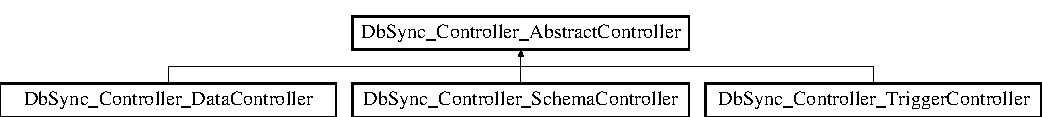
\includegraphics[height=1.568627cm]{classDbSync__Controller__AbstractController}
\end{center}
\end{figure}
\subsection*{Public Member Functions}
\begin{DoxyCompactItemize}
\item 
\hyperlink{classDbSync__Controller__AbstractController_a6afb890b457d835ce2fc37177a73268c}{\_\-\_\-construct} (array \$config)
\item 
\hyperlink{classDbSync__Controller__AbstractController_a26c95d326895bcad46f6b61a3674f5c6}{dispatch} (\hyperlink{classDbSync__Console}{DbSync\_\-Console} \$console)
\item 
\hyperlink{classDbSync__Controller__AbstractController_ac07432b2dbe3854b4f7924fa7887215c}{getItemsList} (\$action)
\item 
\hyperlink{classDbSync__Controller__AbstractController_a40107b1c2a0d5e2f3da236a5c32c2f93}{\_\-\_\-destruct} ()
\item 
\hyperlink{classDbSync__Controller__AbstractController_aaffa31e72a2dcdd6d2a144b8000e7231}{helpAction} ()
\item 
\hyperlink{classDbSync__Controller__AbstractController_aa27d714cc779879c43ca3621c65c65de}{showUsage} ()
\item 
\hyperlink{classDbSync__Controller__AbstractController_a12b74400d214770030c52d2f29308f52}{statusAction} ()
\item 
\hyperlink{classDbSync__Controller__AbstractController_ae973fdc065acffa90f43425b2d480794}{initAction} ()
\item 
\hyperlink{classDbSync__Controller__AbstractController_ab0e568570a013d19ba46b44c4e1e4aa4}{pullAction} ()
\item 
\hyperlink{classDbSync__Controller__AbstractController_a94bd514ad322a37bf6bf2158b98b69b7}{diffAction} ()
\item 
\hyperlink{classDbSync__Controller__AbstractController_abcec7de3ac2e1a43ff35ec2190a9c8d3}{colorize} (\$text, \$color= 'yellow')
\end{DoxyCompactItemize}
\subsection*{Protected Member Functions}
\begin{DoxyCompactItemize}
\item 
\hyperlink{classDbSync__Controller__AbstractController_ae7f065286125487dd51f268138c02113}{\_\-run} (\$action, \$name)
\end{DoxyCompactItemize}
\subsection*{Protected Attributes}
\begin{DoxyCompactItemize}
\item 
\hypertarget{classDbSync__Controller__AbstractController_a419e0e008929c4ac2294a6f90c5965b3}{
{\bfseries \$\_\-modelClass}}
\label{classDbSync__Controller__AbstractController_a419e0e008929c4ac2294a6f90c5965b3}

\item 
\hypertarget{classDbSync__Controller__AbstractController_a499e13fe1d21e988cccccf5497dc0003}{
{\bfseries \$\_\-model}}
\label{classDbSync__Controller__AbstractController_a499e13fe1d21e988cccccf5497dc0003}

\item 
\hypertarget{classDbSync__Controller__AbstractController_a6bd7ca3e9e3faf8da55701916ca82b31}{
{\bfseries \$\_\-console}}
\label{classDbSync__Controller__AbstractController_a6bd7ca3e9e3faf8da55701916ca82b31}

\end{DoxyCompactItemize}


\subsection{Constructor \& Destructor Documentation}
\hypertarget{classDbSync__Controller__AbstractController_a6afb890b457d835ce2fc37177a73268c}{
\index{DbSync\_\-Controller\_\-AbstractController@{DbSync\_\-Controller\_\-AbstractController}!\_\-\_\-construct@{\_\-\_\-construct}}
\index{\_\-\_\-construct@{\_\-\_\-construct}!DbSync_Controller_AbstractController@{DbSync\_\-Controller\_\-AbstractController}}
\subsubsection[{\_\-\_\-construct}]{\setlength{\rightskip}{0pt plus 5cm}DbSync\_\-Controller\_\-AbstractController::\_\-\_\-construct (
\begin{DoxyParamCaption}
\item[{array \$}]{config}
\end{DoxyParamCaption}
)}}
\label{classDbSync__Controller__AbstractController_a6afb890b457d835ce2fc37177a73268c}
Constructor


\begin{DoxyParams}[1]{Parameters}
array & {\em \$config} & \\
\hline
\end{DoxyParams}
\hypertarget{classDbSync__Controller__AbstractController_a40107b1c2a0d5e2f3da236a5c32c2f93}{
\index{DbSync\_\-Controller\_\-AbstractController@{DbSync\_\-Controller\_\-AbstractController}!\_\-\_\-destruct@{\_\-\_\-destruct}}
\index{\_\-\_\-destruct@{\_\-\_\-destruct}!DbSync_Controller_AbstractController@{DbSync\_\-Controller\_\-AbstractController}}
\subsubsection[{\_\-\_\-destruct}]{\setlength{\rightskip}{0pt plus 5cm}DbSync\_\-Controller\_\-AbstractController::\_\-\_\-destruct (
\begin{DoxyParamCaption}
{}
\end{DoxyParamCaption}
)}}
\label{classDbSync__Controller__AbstractController_a40107b1c2a0d5e2f3da236a5c32c2f93}
Descructor 

\subsection{Member Function Documentation}
\hypertarget{classDbSync__Controller__AbstractController_ae7f065286125487dd51f268138c02113}{
\index{DbSync\_\-Controller\_\-AbstractController@{DbSync\_\-Controller\_\-AbstractController}!\_\-run@{\_\-run}}
\index{\_\-run@{\_\-run}!DbSync_Controller_AbstractController@{DbSync\_\-Controller\_\-AbstractController}}
\subsubsection[{\_\-run}]{\setlength{\rightskip}{0pt plus 5cm}DbSync\_\-Controller\_\-AbstractController::\_\-run (
\begin{DoxyParamCaption}
\item[{\$}]{action, }
\item[{\$}]{name}
\end{DoxyParamCaption}
)\hspace{0.3cm}{\ttfamily  \mbox{[}protected\mbox{]}}}}
\label{classDbSync__Controller__AbstractController_ae7f065286125487dd51f268138c02113}
Run action


\begin{DoxyParams}[1]{Parameters}
string & {\em \$action} & \\
\hline
string & {\em \$name} & \\
\hline
\end{DoxyParams}


Reimplemented in \hyperlink{classDbSync__Controller__TriggerController_a2b8ff414b903fc7ac1a433d1f10e2b5a}{DbSync\_\-Controller\_\-TriggerController}.

\hypertarget{classDbSync__Controller__AbstractController_abcec7de3ac2e1a43ff35ec2190a9c8d3}{
\index{DbSync\_\-Controller\_\-AbstractController@{DbSync\_\-Controller\_\-AbstractController}!colorize@{colorize}}
\index{colorize@{colorize}!DbSync_Controller_AbstractController@{DbSync\_\-Controller\_\-AbstractController}}
\subsubsection[{colorize}]{\setlength{\rightskip}{0pt plus 5cm}DbSync\_\-Controller\_\-AbstractController::colorize (
\begin{DoxyParamCaption}
\item[{\$}]{text, }
\item[{\$}]{color = {\ttfamily 'yellow'}}
\end{DoxyParamCaption}
)}}
\label{classDbSync__Controller__AbstractController_abcec7de3ac2e1a43ff35ec2190a9c8d3}
Colorize


\begin{DoxyParams}[1]{Parameters}
string & {\em \$text} & \\
\hline
string & {\em \$color} & \\
\hline
\end{DoxyParams}
\begin{DoxyReturn}{Returns}
string 
\end{DoxyReturn}
\hypertarget{classDbSync__Controller__AbstractController_a94bd514ad322a37bf6bf2158b98b69b7}{
\index{DbSync\_\-Controller\_\-AbstractController@{DbSync\_\-Controller\_\-AbstractController}!diffAction@{diffAction}}
\index{diffAction@{diffAction}!DbSync_Controller_AbstractController@{DbSync\_\-Controller\_\-AbstractController}}
\subsubsection[{diffAction}]{\setlength{\rightskip}{0pt plus 5cm}DbSync\_\-Controller\_\-AbstractController::diffAction (
\begin{DoxyParamCaption}
{}
\end{DoxyParamCaption}
)}}
\label{classDbSync__Controller__AbstractController_a94bd514ad322a37bf6bf2158b98b69b7}
Diff

\begin{DoxyReturn}{Returns}
Show diff between database table schema and schema config file 
\end{DoxyReturn}


Reimplemented in \hyperlink{classDbSync__Controller__TriggerController_a485f3483de2efad7b59b9cb5cef694b4}{DbSync\_\-Controller\_\-TriggerController}.

\hypertarget{classDbSync__Controller__AbstractController_a26c95d326895bcad46f6b61a3674f5c6}{
\index{DbSync\_\-Controller\_\-AbstractController@{DbSync\_\-Controller\_\-AbstractController}!dispatch@{dispatch}}
\index{dispatch@{dispatch}!DbSync_Controller_AbstractController@{DbSync\_\-Controller\_\-AbstractController}}
\subsubsection[{dispatch}]{\setlength{\rightskip}{0pt plus 5cm}DbSync\_\-Controller\_\-AbstractController::dispatch (
\begin{DoxyParamCaption}
\item[{{\bf DbSync\_\-Console} \$}]{console}
\end{DoxyParamCaption}
)}}
\label{classDbSync__Controller__AbstractController_a26c95d326895bcad46f6b61a3674f5c6}
Dispatch


\begin{DoxyParams}[1]{Parameters}
\hyperlink{classDbSync__Console}{DbSync\_\-Console} & {\em \$console} & \\
\hline
\end{DoxyParams}
\begin{DoxyReturn}{Returns}
mixed 
\end{DoxyReturn}
\hypertarget{classDbSync__Controller__AbstractController_ac07432b2dbe3854b4f7924fa7887215c}{
\index{DbSync\_\-Controller\_\-AbstractController@{DbSync\_\-Controller\_\-AbstractController}!getItemsList@{getItemsList}}
\index{getItemsList@{getItemsList}!DbSync_Controller_AbstractController@{DbSync\_\-Controller\_\-AbstractController}}
\subsubsection[{getItemsList}]{\setlength{\rightskip}{0pt plus 5cm}DbSync\_\-Controller\_\-AbstractController::getItemsList (
\begin{DoxyParamCaption}
\item[{\$}]{action}
\end{DoxyParamCaption}
)}}
\label{classDbSync__Controller__AbstractController_ac07432b2dbe3854b4f7924fa7887215c}
Get items list


\begin{DoxyParams}[1]{Parameters}
string & {\em \$action} & \\
\hline
\end{DoxyParams}
\begin{DoxyReturn}{Returns}
array 
\end{DoxyReturn}


Reimplemented in \hyperlink{classDbSync__Controller__TriggerController_a18f4eb165243504cf1354464be4ec9de}{DbSync\_\-Controller\_\-TriggerController}.

\hypertarget{classDbSync__Controller__AbstractController_aaffa31e72a2dcdd6d2a144b8000e7231}{
\index{DbSync\_\-Controller\_\-AbstractController@{DbSync\_\-Controller\_\-AbstractController}!helpAction@{helpAction}}
\index{helpAction@{helpAction}!DbSync_Controller_AbstractController@{DbSync\_\-Controller\_\-AbstractController}}
\subsubsection[{helpAction}]{\setlength{\rightskip}{0pt plus 5cm}DbSync\_\-Controller\_\-AbstractController::helpAction (
\begin{DoxyParamCaption}
{}
\end{DoxyParamCaption}
)}}
\label{classDbSync__Controller__AbstractController_aaffa31e72a2dcdd6d2a144b8000e7231}
Help action

\begin{DoxyReturn}{Returns}
Help message 
\end{DoxyReturn}


Reimplemented in \hyperlink{classDbSync__Controller__TriggerController_a4d53a691eb15f7d060c4db5d14e8c240}{DbSync\_\-Controller\_\-TriggerController}.

\hypertarget{classDbSync__Controller__AbstractController_ae973fdc065acffa90f43425b2d480794}{
\index{DbSync\_\-Controller\_\-AbstractController@{DbSync\_\-Controller\_\-AbstractController}!initAction@{initAction}}
\index{initAction@{initAction}!DbSync_Controller_AbstractController@{DbSync\_\-Controller\_\-AbstractController}}
\subsubsection[{initAction}]{\setlength{\rightskip}{0pt plus 5cm}DbSync\_\-Controller\_\-AbstractController::initAction (
\begin{DoxyParamCaption}
{}
\end{DoxyParamCaption}
)}}
\label{classDbSync__Controller__AbstractController_ae973fdc065acffa90f43425b2d480794}
Init

\begin{DoxyReturn}{Returns}
Create config file(s) 
\end{DoxyReturn}


Reimplemented in \hyperlink{classDbSync__Controller__TriggerController_ac5ee83f5159f52d4327632347a25c2dd}{DbSync\_\-Controller\_\-TriggerController}.

\hypertarget{classDbSync__Controller__AbstractController_ab0e568570a013d19ba46b44c4e1e4aa4}{
\index{DbSync\_\-Controller\_\-AbstractController@{DbSync\_\-Controller\_\-AbstractController}!pullAction@{pullAction}}
\index{pullAction@{pullAction}!DbSync_Controller_AbstractController@{DbSync\_\-Controller\_\-AbstractController}}
\subsubsection[{pullAction}]{\setlength{\rightskip}{0pt plus 5cm}DbSync\_\-Controller\_\-AbstractController::pullAction (
\begin{DoxyParamCaption}
{}
\end{DoxyParamCaption}
)}}
\label{classDbSync__Controller__AbstractController_ab0e568570a013d19ba46b44c4e1e4aa4}
Pull

\begin{DoxyReturn}{Returns}
Override current table config(s) file by new created from database 
\end{DoxyReturn}


Reimplemented in \hyperlink{classDbSync__Controller__TriggerController_ada505e291b61976b9a9a8b3a1b64e998}{DbSync\_\-Controller\_\-TriggerController}.

\hypertarget{classDbSync__Controller__AbstractController_aa27d714cc779879c43ca3621c65c65de}{
\index{DbSync\_\-Controller\_\-AbstractController@{DbSync\_\-Controller\_\-AbstractController}!showUsage@{showUsage}}
\index{showUsage@{showUsage}!DbSync_Controller_AbstractController@{DbSync\_\-Controller\_\-AbstractController}}
\subsubsection[{showUsage}]{\setlength{\rightskip}{0pt plus 5cm}DbSync\_\-Controller\_\-AbstractController::showUsage (
\begin{DoxyParamCaption}
{}
\end{DoxyParamCaption}
)}}
\label{classDbSync__Controller__AbstractController_aa27d714cc779879c43ca3621c65c65de}
Output actions usage message \hypertarget{classDbSync__Controller__AbstractController_a12b74400d214770030c52d2f29308f52}{
\index{DbSync\_\-Controller\_\-AbstractController@{DbSync\_\-Controller\_\-AbstractController}!statusAction@{statusAction}}
\index{statusAction@{statusAction}!DbSync_Controller_AbstractController@{DbSync\_\-Controller\_\-AbstractController}}
\subsubsection[{statusAction}]{\setlength{\rightskip}{0pt plus 5cm}DbSync\_\-Controller\_\-AbstractController::statusAction (
\begin{DoxyParamCaption}
{}
\end{DoxyParamCaption}
)}}
\label{classDbSync__Controller__AbstractController_a12b74400d214770030c52d2f29308f52}
Status

\begin{DoxyReturn}{Returns}
Check sync status (Ok/Unsyncronized) 
\end{DoxyReturn}


Reimplemented in \hyperlink{classDbSync__Controller__TriggerController_a08d8439a825dd363b7fb8df076056f65}{DbSync\_\-Controller\_\-TriggerController}.



The documentation for this class was generated from the following file:\begin{DoxyCompactItemize}
\item 
DbSync/Controller/AbstractController.php\end{DoxyCompactItemize}

\hypertarget{classDbSync__Controller__DataController}{
\section{DbSync\_\-Controller\_\-DataController Class Reference}
\label{classDbSync__Controller__DataController}\index{DbSync\_\-Controller\_\-DataController@{DbSync\_\-Controller\_\-DataController}}
}
Inheritance diagram for DbSync\_\-Controller\_\-DataController:\begin{figure}[H]
\begin{center}
\leavevmode
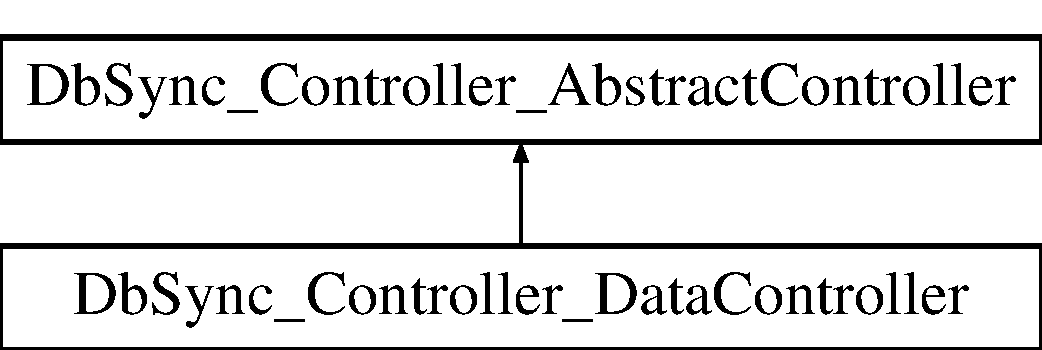
\includegraphics[height=2.000000cm]{classDbSync__Controller__DataController}
\end{center}
\end{figure}
\subsection*{Public Member Functions}
\begin{DoxyCompactItemize}
\item 
\hyperlink{classDbSync__Controller__DataController_a905f98b976e7fa950805cb40f569cbc9}{pushAction} ()
\item 
\hyperlink{classDbSync__Controller__DataController_af83b5323b69423e094c82d965eb72b31}{mergeAction} ()
\end{DoxyCompactItemize}
\subsection*{Protected Attributes}
\begin{DoxyCompactItemize}
\item 
\hypertarget{classDbSync__Controller__DataController_a0ca5fd39aa4db5536a05b5acfcf0d6f9}{
{\bfseries \$\_\-modelClass} = '\hyperlink{classDbSync__Table__Data}{DbSync\_\-Table\_\-Data}'}
\label{classDbSync__Controller__DataController_a0ca5fd39aa4db5536a05b5acfcf0d6f9}

\end{DoxyCompactItemize}


\subsection{Member Function Documentation}
\hypertarget{classDbSync__Controller__DataController_af83b5323b69423e094c82d965eb72b31}{
\index{DbSync\_\-Controller\_\-DataController@{DbSync\_\-Controller\_\-DataController}!mergeAction@{mergeAction}}
\index{mergeAction@{mergeAction}!DbSync_Controller_DataController@{DbSync\_\-Controller\_\-DataController}}
\subsubsection[{mergeAction}]{\setlength{\rightskip}{0pt plus 5cm}DbSync\_\-Controller\_\-DataController::mergeAction (
\begin{DoxyParamCaption}
{}
\end{DoxyParamCaption}
)}}
\label{classDbSync__Controller__DataController_af83b5323b69423e094c82d965eb72b31}
Merge

\begin{DoxyReturn}{Returns}
Merge data rows from config file to database table 
\end{DoxyReturn}
\hypertarget{classDbSync__Controller__DataController_a905f98b976e7fa950805cb40f569cbc9}{
\index{DbSync\_\-Controller\_\-DataController@{DbSync\_\-Controller\_\-DataController}!pushAction@{pushAction}}
\index{pushAction@{pushAction}!DbSync_Controller_DataController@{DbSync\_\-Controller\_\-DataController}}
\subsubsection[{pushAction}]{\setlength{\rightskip}{0pt plus 5cm}DbSync\_\-Controller\_\-DataController::pushAction (
\begin{DoxyParamCaption}
{}
\end{DoxyParamCaption}
)}}
\label{classDbSync__Controller__DataController_a905f98b976e7fa950805cb40f569cbc9}
Push

\begin{DoxyReturn}{Returns}
Override database data by current data config file 

Use \{-\/-\/force$|$yellow\} to truncate table first 
\end{DoxyReturn}


The documentation for this class was generated from the following file:\begin{DoxyCompactItemize}
\item 
DbSync/Controller/DataController.php\end{DoxyCompactItemize}

\hypertarget{classDbSync__Controller__SchemaController}{
\section{DbSync\_\-Controller\_\-SchemaController Class Reference}
\label{classDbSync__Controller__SchemaController}\index{DbSync\_\-Controller\_\-SchemaController@{DbSync\_\-Controller\_\-SchemaController}}
}
Inheritance diagram for DbSync\_\-Controller\_\-SchemaController:\begin{figure}[H]
\begin{center}
\leavevmode
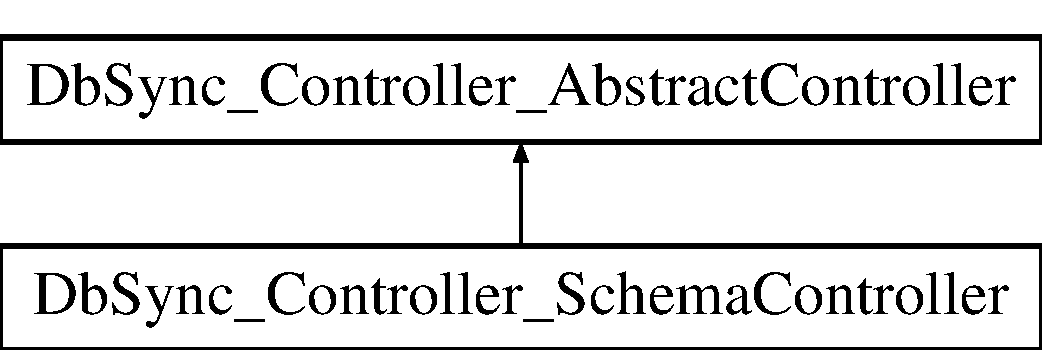
\includegraphics[height=2.000000cm]{classDbSync__Controller__SchemaController}
\end{center}
\end{figure}
\subsection*{Public Member Functions}
\begin{DoxyCompactItemize}
\item 
\hyperlink{classDbSync__Controller__SchemaController_abbd3a6e36859fdb8f8b0a849d284dc81}{deleteAction} ()
\end{DoxyCompactItemize}
\subsection*{Protected Attributes}
\begin{DoxyCompactItemize}
\item 
\hypertarget{classDbSync__Controller__SchemaController_a06640271494bac2c9177a2b87b8a8c13}{
{\bfseries \$\_\-modelClass} = '\hyperlink{classDbSync__Model__Table__Schema}{DbSync\_\-Model\_\-Table\_\-Schema}'}
\label{classDbSync__Controller__SchemaController_a06640271494bac2c9177a2b87b8a8c13}

\end{DoxyCompactItemize}


\subsection{Member Function Documentation}
\hypertarget{classDbSync__Controller__SchemaController_abbd3a6e36859fdb8f8b0a849d284dc81}{
\index{DbSync\_\-Controller\_\-SchemaController@{DbSync\_\-Controller\_\-SchemaController}!deleteAction@{deleteAction}}
\index{deleteAction@{deleteAction}!DbSync_Controller_SchemaController@{DbSync\_\-Controller\_\-SchemaController}}
\subsubsection[{deleteAction}]{\setlength{\rightskip}{0pt plus 5cm}DbSync\_\-Controller\_\-SchemaController::deleteAction (
\begin{DoxyParamCaption}
{}
\end{DoxyParamCaption}
)}}
\label{classDbSync__Controller__SchemaController_abbd3a6e36859fdb8f8b0a849d284dc81}
Delete

de

\begin{DoxyReturn}{Returns}
Delete table and config 

Use \{-\/-\/db$|$yellow\} to delete only form database 

Use \{-\/-\/file$|$yellow\} to delete only config file 
\end{DoxyReturn}


The documentation for this class was generated from the following file:\begin{DoxyCompactItemize}
\item 
DbSync/Controller/SchemaController.php\end{DoxyCompactItemize}

\hypertarget{classDbSync__Controller__TriggerController}{
\section{DbSync\_\-Controller\_\-TriggerController Class Reference}
\label{classDbSync__Controller__TriggerController}\index{DbSync\_\-Controller\_\-TriggerController@{DbSync\_\-Controller\_\-TriggerController}}
}
Inheritance diagram for DbSync\_\-Controller\_\-TriggerController:\begin{figure}[H]
\begin{center}
\leavevmode
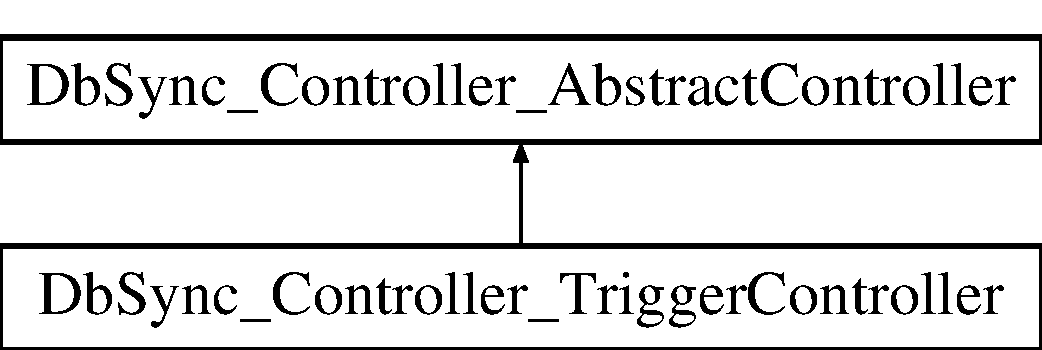
\includegraphics[height=2.000000cm]{classDbSync__Controller__TriggerController}
\end{center}
\end{figure}
\subsection*{Public Member Functions}
\begin{DoxyCompactItemize}
\item 
\hyperlink{classDbSync__Controller__TriggerController_a18f4eb165243504cf1354464be4ec9de}{getItemsList} (\$action)
\item 
\hyperlink{classDbSync__Controller__TriggerController_a4d53a691eb15f7d060c4db5d14e8c240}{helpAction} ()
\item 
\hyperlink{classDbSync__Controller__TriggerController_af0518cd0c76d9ae0a20b44d2a1c311b0}{deleteAction} ()
\item 
\hyperlink{classDbSync__Controller__TriggerController_a08d8439a825dd363b7fb8df076056f65}{statusAction} ()
\end{DoxyCompactItemize}
\subsection*{Protected Member Functions}
\begin{DoxyCompactItemize}
\item 
\hyperlink{classDbSync__Controller__TriggerController_a2b8ff414b903fc7ac1a433d1f10e2b5a}{\_\-run} (\$action, \$name)
\end{DoxyCompactItemize}
\subsection*{Protected Attributes}
\begin{DoxyCompactItemize}
\item 
\hypertarget{classDbSync__Controller__TriggerController_a9e3a9ae192647f811cb45f77e97af78d}{
{\bfseries \$\_\-modelClass} = '\hyperlink{classDbSync__Model__Table__Trigger}{DbSync\_\-Model\_\-Table\_\-Trigger}'}
\label{classDbSync__Controller__TriggerController_a9e3a9ae192647f811cb45f77e97af78d}

\item 
\hypertarget{classDbSync__Controller__TriggerController_a5b69850f05d66f66508a58bf60ee1378}{
{\bfseries \$\_\-model}}
\label{classDbSync__Controller__TriggerController_a5b69850f05d66f66508a58bf60ee1378}

\end{DoxyCompactItemize}


\subsection{Member Function Documentation}
\hypertarget{classDbSync__Controller__TriggerController_a2b8ff414b903fc7ac1a433d1f10e2b5a}{
\index{DbSync\_\-Controller\_\-TriggerController@{DbSync\_\-Controller\_\-TriggerController}!\_\-run@{\_\-run}}
\index{\_\-run@{\_\-run}!DbSync_Controller_TriggerController@{DbSync\_\-Controller\_\-TriggerController}}
\subsubsection[{\_\-run}]{\setlength{\rightskip}{0pt plus 5cm}DbSync\_\-Controller\_\-TriggerController::\_\-run (
\begin{DoxyParamCaption}
\item[{\$}]{action, }
\item[{\$}]{name}
\end{DoxyParamCaption}
)\hspace{0.3cm}{\ttfamily  \mbox{[}protected\mbox{]}}}}
\label{classDbSync__Controller__TriggerController_a2b8ff414b903fc7ac1a433d1f10e2b5a}
Run action


\begin{DoxyParams}[1]{Parameters}
string & {\em \$action} & \\
\hline
string & {\em \$name} & \\
\hline
\end{DoxyParams}


Reimplemented from \hyperlink{classDbSync__Controller__AbstractController_ae7f065286125487dd51f268138c02113}{DbSync\_\-Controller\_\-AbstractController}.

\hypertarget{classDbSync__Controller__TriggerController_af0518cd0c76d9ae0a20b44d2a1c311b0}{
\index{DbSync\_\-Controller\_\-TriggerController@{DbSync\_\-Controller\_\-TriggerController}!deleteAction@{deleteAction}}
\index{deleteAction@{deleteAction}!DbSync_Controller_TriggerController@{DbSync\_\-Controller\_\-TriggerController}}
\subsubsection[{deleteAction}]{\setlength{\rightskip}{0pt plus 5cm}DbSync\_\-Controller\_\-TriggerController::deleteAction (
\begin{DoxyParamCaption}
{}
\end{DoxyParamCaption}
)}}
\label{classDbSync__Controller__TriggerController_af0518cd0c76d9ae0a20b44d2a1c311b0}
Delete

de

\begin{DoxyReturn}{Returns}
Delete trigger and config 

Use \{-\/-\/db$|$yellow\} to delete only from database 

Use \{-\/-\/file$|$yellow\} to delete only config file 
\end{DoxyReturn}
\hypertarget{classDbSync__Controller__TriggerController_a18f4eb165243504cf1354464be4ec9de}{
\index{DbSync\_\-Controller\_\-TriggerController@{DbSync\_\-Controller\_\-TriggerController}!getItemsList@{getItemsList}}
\index{getItemsList@{getItemsList}!DbSync_Controller_TriggerController@{DbSync\_\-Controller\_\-TriggerController}}
\subsubsection[{getItemsList}]{\setlength{\rightskip}{0pt plus 5cm}DbSync\_\-Controller\_\-TriggerController::getItemsList (
\begin{DoxyParamCaption}
\item[{\$}]{action}
\end{DoxyParamCaption}
)}}
\label{classDbSync__Controller__TriggerController_a18f4eb165243504cf1354464be4ec9de}
Get items list


\begin{DoxyParams}[1]{Parameters}
string & {\em \$action} & \\
\hline
\end{DoxyParams}
\begin{DoxyReturn}{Returns}
array 
\end{DoxyReturn}


Reimplemented from \hyperlink{classDbSync__Controller__AbstractController_ac07432b2dbe3854b4f7924fa7887215c}{DbSync\_\-Controller\_\-AbstractController}.

\hypertarget{classDbSync__Controller__TriggerController_a4d53a691eb15f7d060c4db5d14e8c240}{
\index{DbSync\_\-Controller\_\-TriggerController@{DbSync\_\-Controller\_\-TriggerController}!helpAction@{helpAction}}
\index{helpAction@{helpAction}!DbSync_Controller_TriggerController@{DbSync\_\-Controller\_\-TriggerController}}
\subsubsection[{helpAction}]{\setlength{\rightskip}{0pt plus 5cm}DbSync\_\-Controller\_\-TriggerController::helpAction (
\begin{DoxyParamCaption}
{}
\end{DoxyParamCaption}
)}}
\label{classDbSync__Controller__TriggerController_a4d53a691eb15f7d060c4db5d14e8c240}
Help

\begin{DoxyReturn}{Returns}
Help message 
\end{DoxyReturn}
\begin{DoxySeeAlso}{See also}
DbSync\_\-Controller::help() 
\end{DoxySeeAlso}


Reimplemented from \hyperlink{classDbSync__Controller__AbstractController_aaffa31e72a2dcdd6d2a144b8000e7231}{DbSync\_\-Controller\_\-AbstractController}.

\hypertarget{classDbSync__Controller__TriggerController_a08d8439a825dd363b7fb8df076056f65}{
\index{DbSync\_\-Controller\_\-TriggerController@{DbSync\_\-Controller\_\-TriggerController}!statusAction@{statusAction}}
\index{statusAction@{statusAction}!DbSync_Controller_TriggerController@{DbSync\_\-Controller\_\-TriggerController}}
\subsubsection[{statusAction}]{\setlength{\rightskip}{0pt plus 5cm}DbSync\_\-Controller\_\-TriggerController::statusAction (
\begin{DoxyParamCaption}
{}
\end{DoxyParamCaption}
)}}
\label{classDbSync__Controller__TriggerController_a08d8439a825dd363b7fb8df076056f65}
Status

st

\begin{DoxyReturn}{Returns}
Check triggers status (Ok/Unsyncronized) 

Use \{-\/-\/table \mbox{[}\mbox{[}tableName\mbox{]} ... \mbox{]}$|$yellow\} to display triggers for certain table(s) 
\end{DoxyReturn}


Reimplemented from \hyperlink{classDbSync__Controller__AbstractController_a12b74400d214770030c52d2f29308f52}{DbSync\_\-Controller\_\-AbstractController}.



The documentation for this class was generated from the following file:\begin{DoxyCompactItemize}
\item 
DbSync/Controller/TriggerController.php\end{DoxyCompactItemize}

\hypertarget{interfaceDbSync__DbAdapter__AdapterInterface}{
\section{DbSync\_\-DbAdapter\_\-AdapterInterface Interface Reference}
\label{interfaceDbSync__DbAdapter__AdapterInterface}\index{DbSync\_\-DbAdapter\_\-AdapterInterface@{DbSync\_\-DbAdapter\_\-AdapterInterface}}
}
Inheritance diagram for DbSync\_\-DbAdapter\_\-AdapterInterface:\begin{figure}[H]
\begin{center}
\leavevmode
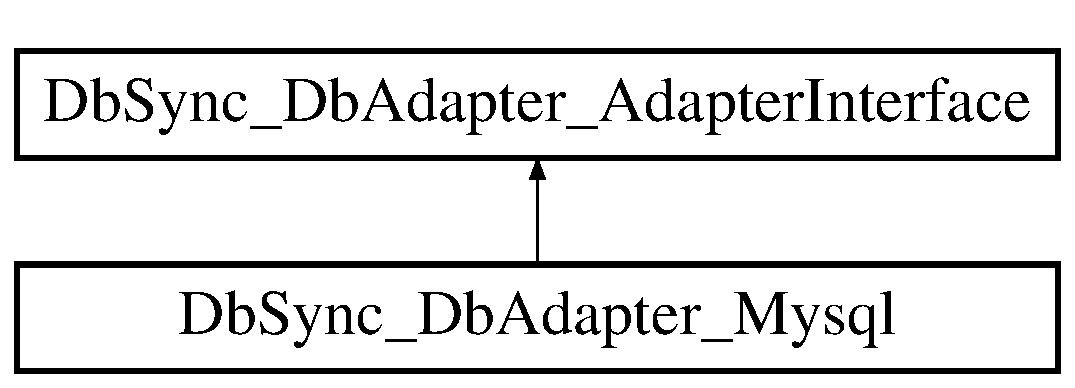
\includegraphics[height=2.000000cm]{interfaceDbSync__DbAdapter__AdapterInterface}
\end{center}
\end{figure}
\subsection*{Public Member Functions}
\begin{DoxyCompactItemize}
\item 
\hyperlink{interfaceDbSync__DbAdapter__AdapterInterface_a29aeee3cbdac7e08ca3c08f464f5b443}{\_\-\_\-construct} (array \$config)
\item 
\hyperlink{interfaceDbSync__DbAdapter__AdapterInterface_a683e550d89b21e02e4068993f30079fc}{parseSchema} (\$tableName)
\item 
\hyperlink{interfaceDbSync__DbAdapter__AdapterInterface_acc0350206ef7c623402bb19633ad3f6a}{createAlter} (\$config, \$tableName)
\item 
\hyperlink{interfaceDbSync__DbAdapter__AdapterInterface_acea54c81f65be6ea4eceb8dcf3b93659}{parseTrigger} (\$triggerName)
\item 
\hyperlink{interfaceDbSync__DbAdapter__AdapterInterface_a2efd82563860bf45fc07fbeb4d67b056}{createTriggerSql} (\$config)
\item 
\hyperlink{interfaceDbSync__DbAdapter__AdapterInterface_a4e19047119e11123e47f8c8c14e0c665}{execute} (\$sql)
\item 
\hyperlink{interfaceDbSync__DbAdapter__AdapterInterface_a686c3e752907a09cc1d87fce2d2bb101}{getTriggerList} ()
\item 
\hyperlink{interfaceDbSync__DbAdapter__AdapterInterface_a6df405111c98ca40324423f8981d7974}{getTableByTrigger} (\$triggerName)
\item 
\hyperlink{interfaceDbSync__DbAdapter__AdapterInterface_a84b87f76dc8ebc123d42dda7393e0cb9}{getTableList} ()
\item 
\hyperlink{interfaceDbSync__DbAdapter__AdapterInterface_ac1cb4888b127b104ed231feae87d3056}{hasTable} (\$tableName)
\item 
\hyperlink{interfaceDbSync__DbAdapter__AdapterInterface_aa8f4119b6cc6cf5bfd0d97d45a849d9d}{hasTrigger} (\$triggerName)
\item 
\hyperlink{interfaceDbSync__DbAdapter__AdapterInterface_ad60b6d7e34fba4e763132e47134b35e1}{fetchData} (\$tableName)
\item 
\hyperlink{interfaceDbSync__DbAdapter__AdapterInterface_ad535c5d4d074383feb578fab1e71d2e7}{insert} (\$data, \$tableName)
\item 
\hyperlink{interfaceDbSync__DbAdapter__AdapterInterface_a06dfb3597de81841661535373ce06e0d}{merge} (\$data, \$tableName)
\item 
\hyperlink{interfaceDbSync__DbAdapter__AdapterInterface_a2cc0eb5ae7c4aa0b69a899e84040da83}{truncate} (\$tableName)
\item 
\hyperlink{interfaceDbSync__DbAdapter__AdapterInterface_a18ccca4e55a874ed85acd00506f4fff2}{dropTable} (\$tableName)
\item 
\hyperlink{interfaceDbSync__DbAdapter__AdapterInterface_afb0b32f718a3a499955444966929997b}{dropTrigger} (\$triggerName)
\item 
\hyperlink{interfaceDbSync__DbAdapter__AdapterInterface_abe0d20fb62067de68fb354adc3eb7e8a}{isEmpty} (\$tableName)
\end{DoxyCompactItemize}


\subsection{Constructor \& Destructor Documentation}
\hypertarget{interfaceDbSync__DbAdapter__AdapterInterface_a29aeee3cbdac7e08ca3c08f464f5b443}{
\index{DbSync\_\-DbAdapter\_\-AdapterInterface@{DbSync\_\-DbAdapter\_\-AdapterInterface}!\_\-\_\-construct@{\_\-\_\-construct}}
\index{\_\-\_\-construct@{\_\-\_\-construct}!DbSync_DbAdapter_AdapterInterface@{DbSync\_\-DbAdapter\_\-AdapterInterface}}
\subsubsection[{\_\-\_\-construct}]{\setlength{\rightskip}{0pt plus 5cm}DbSync\_\-DbAdapter\_\-AdapterInterface::\_\-\_\-construct (
\begin{DoxyParamCaption}
\item[{array \$}]{config}
\end{DoxyParamCaption}
)}}
\label{interfaceDbSync__DbAdapter__AdapterInterface_a29aeee3cbdac7e08ca3c08f464f5b443}
Constructor


\begin{DoxyParams}[1]{Parameters}
array & {\em \$config} & \\
\hline
\end{DoxyParams}


Implemented in \hyperlink{classDbSync__DbAdapter__Mysql_abf098ec8f68514927dacce23e5a30030}{DbSync\_\-DbAdapter\_\-Mysql}.



\subsection{Member Function Documentation}
\hypertarget{interfaceDbSync__DbAdapter__AdapterInterface_acc0350206ef7c623402bb19633ad3f6a}{
\index{DbSync\_\-DbAdapter\_\-AdapterInterface@{DbSync\_\-DbAdapter\_\-AdapterInterface}!createAlter@{createAlter}}
\index{createAlter@{createAlter}!DbSync_DbAdapter_AdapterInterface@{DbSync\_\-DbAdapter\_\-AdapterInterface}}
\subsubsection[{createAlter}]{\setlength{\rightskip}{0pt plus 5cm}DbSync\_\-DbAdapter\_\-AdapterInterface::createAlter (
\begin{DoxyParamCaption}
\item[{\$}]{config, }
\item[{\$}]{tableName}
\end{DoxyParamCaption}
)}}
\label{interfaceDbSync__DbAdapter__AdapterInterface_acc0350206ef7c623402bb19633ad3f6a}
Generate Alter Table


\begin{DoxyParams}[1]{Parameters}
array & {\em \$config} & \\
\hline
string & {\em \$tableName} & \\
\hline
\end{DoxyParams}
\begin{DoxyReturn}{Returns}
string 
\end{DoxyReturn}


Implemented in \hyperlink{classDbSync__DbAdapter__Mysql_a51b9a8196dcbef50547417d4fe8a0666}{DbSync\_\-DbAdapter\_\-Mysql}.

\hypertarget{interfaceDbSync__DbAdapter__AdapterInterface_a2efd82563860bf45fc07fbeb4d67b056}{
\index{DbSync\_\-DbAdapter\_\-AdapterInterface@{DbSync\_\-DbAdapter\_\-AdapterInterface}!createTriggerSql@{createTriggerSql}}
\index{createTriggerSql@{createTriggerSql}!DbSync_DbAdapter_AdapterInterface@{DbSync\_\-DbAdapter\_\-AdapterInterface}}
\subsubsection[{createTriggerSql}]{\setlength{\rightskip}{0pt plus 5cm}DbSync\_\-DbAdapter\_\-AdapterInterface::createTriggerSql (
\begin{DoxyParamCaption}
\item[{\$}]{config}
\end{DoxyParamCaption}
)}}
\label{interfaceDbSync__DbAdapter__AdapterInterface_a2efd82563860bf45fc07fbeb4d67b056}
Generate trigger sql


\begin{DoxyParams}[1]{Parameters}
array & {\em \$config} & \\
\hline
\end{DoxyParams}
\begin{DoxyReturn}{Returns}
string 
\end{DoxyReturn}


Implemented in \hyperlink{classDbSync__DbAdapter__Mysql_af58ff620be0d1f4cac9b865ca0000fcf}{DbSync\_\-DbAdapter\_\-Mysql}.

\hypertarget{interfaceDbSync__DbAdapter__AdapterInterface_a18ccca4e55a874ed85acd00506f4fff2}{
\index{DbSync\_\-DbAdapter\_\-AdapterInterface@{DbSync\_\-DbAdapter\_\-AdapterInterface}!dropTable@{dropTable}}
\index{dropTable@{dropTable}!DbSync_DbAdapter_AdapterInterface@{DbSync\_\-DbAdapter\_\-AdapterInterface}}
\subsubsection[{dropTable}]{\setlength{\rightskip}{0pt plus 5cm}DbSync\_\-DbAdapter\_\-AdapterInterface::dropTable (
\begin{DoxyParamCaption}
\item[{\$}]{tableName}
\end{DoxyParamCaption}
)}}
\label{interfaceDbSync__DbAdapter__AdapterInterface_a18ccca4e55a874ed85acd00506f4fff2}
Drop table


\begin{DoxyParams}[1]{Parameters}
string & {\em \$tableName} & \\
\hline
\end{DoxyParams}
\begin{DoxyReturn}{Returns}
number 
\end{DoxyReturn}


Implemented in \hyperlink{classDbSync__DbAdapter__Mysql_a95bec76ffdfe365cc68a682724443488}{DbSync\_\-DbAdapter\_\-Mysql}.

\hypertarget{interfaceDbSync__DbAdapter__AdapterInterface_afb0b32f718a3a499955444966929997b}{
\index{DbSync\_\-DbAdapter\_\-AdapterInterface@{DbSync\_\-DbAdapter\_\-AdapterInterface}!dropTrigger@{dropTrigger}}
\index{dropTrigger@{dropTrigger}!DbSync_DbAdapter_AdapterInterface@{DbSync\_\-DbAdapter\_\-AdapterInterface}}
\subsubsection[{dropTrigger}]{\setlength{\rightskip}{0pt plus 5cm}DbSync\_\-DbAdapter\_\-AdapterInterface::dropTrigger (
\begin{DoxyParamCaption}
\item[{\$}]{triggerName}
\end{DoxyParamCaption}
)}}
\label{interfaceDbSync__DbAdapter__AdapterInterface_afb0b32f718a3a499955444966929997b}
Drop trigger


\begin{DoxyParams}[1]{Parameters}
string & {\em \$triggerName} & \\
\hline
\end{DoxyParams}
\begin{DoxyReturn}{Returns}
number 
\end{DoxyReturn}


Implemented in \hyperlink{classDbSync__DbAdapter__Mysql_a9a98e8e32ececd6cc3b101d5cc87fa4f}{DbSync\_\-DbAdapter\_\-Mysql}.

\hypertarget{interfaceDbSync__DbAdapter__AdapterInterface_a4e19047119e11123e47f8c8c14e0c665}{
\index{DbSync\_\-DbAdapter\_\-AdapterInterface@{DbSync\_\-DbAdapter\_\-AdapterInterface}!execute@{execute}}
\index{execute@{execute}!DbSync_DbAdapter_AdapterInterface@{DbSync\_\-DbAdapter\_\-AdapterInterface}}
\subsubsection[{execute}]{\setlength{\rightskip}{0pt plus 5cm}DbSync\_\-DbAdapter\_\-AdapterInterface::execute (
\begin{DoxyParamCaption}
\item[{\$}]{sql}
\end{DoxyParamCaption}
)}}
\label{interfaceDbSync__DbAdapter__AdapterInterface_a4e19047119e11123e47f8c8c14e0c665}
Execute sql query


\begin{DoxyParams}[1]{Parameters}
string & {\em \$sql} & \\
\hline
\end{DoxyParams}
\begin{DoxyReturn}{Returns}
integer 
\end{DoxyReturn}


Implemented in \hyperlink{classDbSync__DbAdapter__Mysql_a279036935ed06d1cd41c4ec1d8b107cc}{DbSync\_\-DbAdapter\_\-Mysql}.

\hypertarget{interfaceDbSync__DbAdapter__AdapterInterface_ad60b6d7e34fba4e763132e47134b35e1}{
\index{DbSync\_\-DbAdapter\_\-AdapterInterface@{DbSync\_\-DbAdapter\_\-AdapterInterface}!fetchData@{fetchData}}
\index{fetchData@{fetchData}!DbSync_DbAdapter_AdapterInterface@{DbSync\_\-DbAdapter\_\-AdapterInterface}}
\subsubsection[{fetchData}]{\setlength{\rightskip}{0pt plus 5cm}DbSync\_\-DbAdapter\_\-AdapterInterface::fetchData (
\begin{DoxyParamCaption}
\item[{\$}]{tableName}
\end{DoxyParamCaption}
)}}
\label{interfaceDbSync__DbAdapter__AdapterInterface_ad60b6d7e34fba4e763132e47134b35e1}
Fetch all data from table

\begin{DoxyReturn}{Returns}
array 
\end{DoxyReturn}


Implemented in \hyperlink{classDbSync__DbAdapter__Mysql_a76d3e3c3e80fee76c7057724a55a8d58}{DbSync\_\-DbAdapter\_\-Mysql}.

\hypertarget{interfaceDbSync__DbAdapter__AdapterInterface_a6df405111c98ca40324423f8981d7974}{
\index{DbSync\_\-DbAdapter\_\-AdapterInterface@{DbSync\_\-DbAdapter\_\-AdapterInterface}!getTableByTrigger@{getTableByTrigger}}
\index{getTableByTrigger@{getTableByTrigger}!DbSync_DbAdapter_AdapterInterface@{DbSync\_\-DbAdapter\_\-AdapterInterface}}
\subsubsection[{getTableByTrigger}]{\setlength{\rightskip}{0pt plus 5cm}DbSync\_\-DbAdapter\_\-AdapterInterface::getTableByTrigger (
\begin{DoxyParamCaption}
\item[{\$}]{triggerName}
\end{DoxyParamCaption}
)}}
\label{interfaceDbSync__DbAdapter__AdapterInterface_a6df405111c98ca40324423f8981d7974}
Get table name by trigger name

\begin{DoxyReturn}{Returns}
string 
\end{DoxyReturn}


Implemented in \hyperlink{classDbSync__DbAdapter__Mysql_a1bb1fb6762c987d2bdcd243c37875a54}{DbSync\_\-DbAdapter\_\-Mysql}.

\hypertarget{interfaceDbSync__DbAdapter__AdapterInterface_a84b87f76dc8ebc123d42dda7393e0cb9}{
\index{DbSync\_\-DbAdapter\_\-AdapterInterface@{DbSync\_\-DbAdapter\_\-AdapterInterface}!getTableList@{getTableList}}
\index{getTableList@{getTableList}!DbSync_DbAdapter_AdapterInterface@{DbSync\_\-DbAdapter\_\-AdapterInterface}}
\subsubsection[{getTableList}]{\setlength{\rightskip}{0pt plus 5cm}DbSync\_\-DbAdapter\_\-AdapterInterface::getTableList (
\begin{DoxyParamCaption}
{}
\end{DoxyParamCaption}
)}}
\label{interfaceDbSync__DbAdapter__AdapterInterface_a84b87f76dc8ebc123d42dda7393e0cb9}
Get tables list

\begin{DoxyReturn}{Returns}
array 
\end{DoxyReturn}


Implemented in \hyperlink{classDbSync__DbAdapter__Mysql_ab6a45a23420b3f1e5817fbe287c53842}{DbSync\_\-DbAdapter\_\-Mysql}.

\hypertarget{interfaceDbSync__DbAdapter__AdapterInterface_a686c3e752907a09cc1d87fce2d2bb101}{
\index{DbSync\_\-DbAdapter\_\-AdapterInterface@{DbSync\_\-DbAdapter\_\-AdapterInterface}!getTriggerList@{getTriggerList}}
\index{getTriggerList@{getTriggerList}!DbSync_DbAdapter_AdapterInterface@{DbSync\_\-DbAdapter\_\-AdapterInterface}}
\subsubsection[{getTriggerList}]{\setlength{\rightskip}{0pt plus 5cm}DbSync\_\-DbAdapter\_\-AdapterInterface::getTriggerList (
\begin{DoxyParamCaption}
{}
\end{DoxyParamCaption}
)}}
\label{interfaceDbSync__DbAdapter__AdapterInterface_a686c3e752907a09cc1d87fce2d2bb101}
Get triggers list

\begin{DoxyReturn}{Returns}
array 
\end{DoxyReturn}
\hypertarget{interfaceDbSync__DbAdapter__AdapterInterface_ac1cb4888b127b104ed231feae87d3056}{
\index{DbSync\_\-DbAdapter\_\-AdapterInterface@{DbSync\_\-DbAdapter\_\-AdapterInterface}!hasTable@{hasTable}}
\index{hasTable@{hasTable}!DbSync_DbAdapter_AdapterInterface@{DbSync\_\-DbAdapter\_\-AdapterInterface}}
\subsubsection[{hasTable}]{\setlength{\rightskip}{0pt plus 5cm}DbSync\_\-DbAdapter\_\-AdapterInterface::hasTable (
\begin{DoxyParamCaption}
\item[{\$}]{tableName}
\end{DoxyParamCaption}
)}}
\label{interfaceDbSync__DbAdapter__AdapterInterface_ac1cb4888b127b104ed231feae87d3056}
Is db table exists

\begin{DoxyReturn}{Returns}
boolen 
\end{DoxyReturn}


Implemented in \hyperlink{classDbSync__DbAdapter__Mysql_aceee5101dd14398aa51b7f3abfe88306}{DbSync\_\-DbAdapter\_\-Mysql}.

\hypertarget{interfaceDbSync__DbAdapter__AdapterInterface_aa8f4119b6cc6cf5bfd0d97d45a849d9d}{
\index{DbSync\_\-DbAdapter\_\-AdapterInterface@{DbSync\_\-DbAdapter\_\-AdapterInterface}!hasTrigger@{hasTrigger}}
\index{hasTrigger@{hasTrigger}!DbSync_DbAdapter_AdapterInterface@{DbSync\_\-DbAdapter\_\-AdapterInterface}}
\subsubsection[{hasTrigger}]{\setlength{\rightskip}{0pt plus 5cm}DbSync\_\-DbAdapter\_\-AdapterInterface::hasTrigger (
\begin{DoxyParamCaption}
\item[{\$}]{triggerName}
\end{DoxyParamCaption}
)}}
\label{interfaceDbSync__DbAdapter__AdapterInterface_aa8f4119b6cc6cf5bfd0d97d45a849d9d}
Is db trigger exists

\begin{DoxyReturn}{Returns}
boolen 
\end{DoxyReturn}


Implemented in \hyperlink{classDbSync__DbAdapter__Mysql_a7c89b938e8554a37e1244207cb75b3ff}{DbSync\_\-DbAdapter\_\-Mysql}.

\hypertarget{interfaceDbSync__DbAdapter__AdapterInterface_ad535c5d4d074383feb578fab1e71d2e7}{
\index{DbSync\_\-DbAdapter\_\-AdapterInterface@{DbSync\_\-DbAdapter\_\-AdapterInterface}!insert@{insert}}
\index{insert@{insert}!DbSync_DbAdapter_AdapterInterface@{DbSync\_\-DbAdapter\_\-AdapterInterface}}
\subsubsection[{insert}]{\setlength{\rightskip}{0pt plus 5cm}DbSync\_\-DbAdapter\_\-AdapterInterface::insert (
\begin{DoxyParamCaption}
\item[{\$}]{data, }
\item[{\$}]{tableName}
\end{DoxyParamCaption}
)}}
\label{interfaceDbSync__DbAdapter__AdapterInterface_ad535c5d4d074383feb578fab1e71d2e7}
Push data to db table


\begin{DoxyParams}[1]{Parameters}
boolen & {\em \$force} & \\
\hline
\end{DoxyParams}
\begin{DoxyReturn}{Returns}
boolen 
\end{DoxyReturn}

\begin{DoxyExceptions}{Exceptions}
{\em Exception} & \\
\hline
\end{DoxyExceptions}


Implemented in \hyperlink{classDbSync__DbAdapter__Mysql_a5f9f2976276f71419539cb1da154f5de}{DbSync\_\-DbAdapter\_\-Mysql}.

\hypertarget{interfaceDbSync__DbAdapter__AdapterInterface_abe0d20fb62067de68fb354adc3eb7e8a}{
\index{DbSync\_\-DbAdapter\_\-AdapterInterface@{DbSync\_\-DbAdapter\_\-AdapterInterface}!isEmpty@{isEmpty}}
\index{isEmpty@{isEmpty}!DbSync_DbAdapter_AdapterInterface@{DbSync\_\-DbAdapter\_\-AdapterInterface}}
\subsubsection[{isEmpty}]{\setlength{\rightskip}{0pt plus 5cm}DbSync\_\-DbAdapter\_\-AdapterInterface::isEmpty (
\begin{DoxyParamCaption}
\item[{\$}]{tableName}
\end{DoxyParamCaption}
)}}
\label{interfaceDbSync__DbAdapter__AdapterInterface_abe0d20fb62067de68fb354adc3eb7e8a}
Is db table empty


\begin{DoxyParams}[1]{Parameters}
string & {\em \$tableName} & \\
\hline
\end{DoxyParams}
\begin{DoxyReturn}{Returns}
boolean 
\end{DoxyReturn}


Implemented in \hyperlink{classDbSync__DbAdapter__Mysql_ab8b4ba488780a70e219b04cb893549df}{DbSync\_\-DbAdapter\_\-Mysql}.

\hypertarget{interfaceDbSync__DbAdapter__AdapterInterface_a06dfb3597de81841661535373ce06e0d}{
\index{DbSync\_\-DbAdapter\_\-AdapterInterface@{DbSync\_\-DbAdapter\_\-AdapterInterface}!merge@{merge}}
\index{merge@{merge}!DbSync_DbAdapter_AdapterInterface@{DbSync\_\-DbAdapter\_\-AdapterInterface}}
\subsubsection[{merge}]{\setlength{\rightskip}{0pt plus 5cm}DbSync\_\-DbAdapter\_\-AdapterInterface::merge (
\begin{DoxyParamCaption}
\item[{\$}]{data, }
\item[{\$}]{tableName}
\end{DoxyParamCaption}
)}}
\label{interfaceDbSync__DbAdapter__AdapterInterface_a06dfb3597de81841661535373ce06e0d}
Merge data to db table


\begin{DoxyExceptions}{Exceptions}
{\em Exception} & \\
\hline
\end{DoxyExceptions}
\begin{DoxyReturn}{Returns}
boolean 
\end{DoxyReturn}


Implemented in \hyperlink{classDbSync__DbAdapter__Mysql_a8a92a7e594687733c08bacd9d4217521}{DbSync\_\-DbAdapter\_\-Mysql}.

\hypertarget{interfaceDbSync__DbAdapter__AdapterInterface_a683e550d89b21e02e4068993f30079fc}{
\index{DbSync\_\-DbAdapter\_\-AdapterInterface@{DbSync\_\-DbAdapter\_\-AdapterInterface}!parseSchema@{parseSchema}}
\index{parseSchema@{parseSchema}!DbSync_DbAdapter_AdapterInterface@{DbSync\_\-DbAdapter\_\-AdapterInterface}}
\subsubsection[{parseSchema}]{\setlength{\rightskip}{0pt plus 5cm}DbSync\_\-DbAdapter\_\-AdapterInterface::parseSchema (
\begin{DoxyParamCaption}
\item[{\$}]{tableName}
\end{DoxyParamCaption}
)}}
\label{interfaceDbSync__DbAdapter__AdapterInterface_a683e550d89b21e02e4068993f30079fc}
Parse schema

\begin{DoxyReturn}{Returns}
array 
\end{DoxyReturn}


Implemented in \hyperlink{classDbSync__DbAdapter__Mysql_a1eeb0ab74018b405fdd42ba5c37adc2d}{DbSync\_\-DbAdapter\_\-Mysql}.

\hypertarget{interfaceDbSync__DbAdapter__AdapterInterface_acea54c81f65be6ea4eceb8dcf3b93659}{
\index{DbSync\_\-DbAdapter\_\-AdapterInterface@{DbSync\_\-DbAdapter\_\-AdapterInterface}!parseTrigger@{parseTrigger}}
\index{parseTrigger@{parseTrigger}!DbSync_DbAdapter_AdapterInterface@{DbSync\_\-DbAdapter\_\-AdapterInterface}}
\subsubsection[{parseTrigger}]{\setlength{\rightskip}{0pt plus 5cm}DbSync\_\-DbAdapter\_\-AdapterInterface::parseTrigger (
\begin{DoxyParamCaption}
\item[{\$}]{triggerName}
\end{DoxyParamCaption}
)}}
\label{interfaceDbSync__DbAdapter__AdapterInterface_acea54c81f65be6ea4eceb8dcf3b93659}
Fetch db triggers

\begin{DoxyReturn}{Returns}
string 
\end{DoxyReturn}


Implemented in \hyperlink{classDbSync__DbAdapter__Mysql_acf8d25625a74af2fe9f31e4b621ef0f0}{DbSync\_\-DbAdapter\_\-Mysql}.

\hypertarget{interfaceDbSync__DbAdapter__AdapterInterface_a2cc0eb5ae7c4aa0b69a899e84040da83}{
\index{DbSync\_\-DbAdapter\_\-AdapterInterface@{DbSync\_\-DbAdapter\_\-AdapterInterface}!truncate@{truncate}}
\index{truncate@{truncate}!DbSync_DbAdapter_AdapterInterface@{DbSync\_\-DbAdapter\_\-AdapterInterface}}
\subsubsection[{truncate}]{\setlength{\rightskip}{0pt plus 5cm}DbSync\_\-DbAdapter\_\-AdapterInterface::truncate (
\begin{DoxyParamCaption}
\item[{\$}]{tableName}
\end{DoxyParamCaption}
)}}
\label{interfaceDbSync__DbAdapter__AdapterInterface_a2cc0eb5ae7c4aa0b69a899e84040da83}
Truncate table


\begin{DoxyParams}[1]{Parameters}
string & {\em \$tableName} & \\
\hline
\end{DoxyParams}
\begin{DoxyReturn}{Returns}
number 
\end{DoxyReturn}


Implemented in \hyperlink{classDbSync__DbAdapter__Mysql_afb653194c5832eb8205adb4fe13a35db}{DbSync\_\-DbAdapter\_\-Mysql}.



The documentation for this interface was generated from the following file:\begin{DoxyCompactItemize}
\item 
DbSync/DbAdapter/AdapterInterface.php\end{DoxyCompactItemize}

\hypertarget{classDbSync__DbAdapter__Mysql}{
\section{DbSync\_\-DbAdapter\_\-Mysql Class Reference}
\label{classDbSync__DbAdapter__Mysql}\index{DbSync\_\-DbAdapter\_\-Mysql@{DbSync\_\-DbAdapter\_\-Mysql}}
}
Inheritance diagram for DbSync\_\-DbAdapter\_\-Mysql:\begin{figure}[H]
\begin{center}
\leavevmode
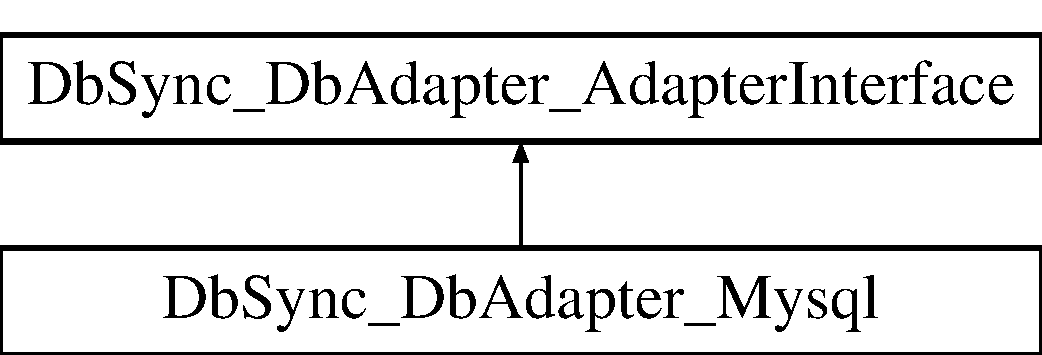
\includegraphics[height=2.000000cm]{classDbSync__DbAdapter__Mysql}
\end{center}
\end{figure}
\subsection*{Public Member Functions}
\begin{DoxyCompactItemize}
\item 
\hyperlink{classDbSync__DbAdapter__Mysql_abf098ec8f68514927dacce23e5a30030}{\_\-\_\-construct} (array \$config)
\item 
\hyperlink{classDbSync__DbAdapter__Mysql_a710f43c8e7cacc9ce8b131b4c0bd9107}{getConnection} ()
\item 
\hyperlink{classDbSync__DbAdapter__Mysql_a62b30dac592a365506212d632a26db1e}{setConnection} (PDO \$connection)
\item 
\hyperlink{classDbSync__DbAdapter__Mysql_a1eeb0ab74018b405fdd42ba5c37adc2d}{parseSchema} (\$tableName)
\item 
\hyperlink{classDbSync__DbAdapter__Mysql_a51b9a8196dcbef50547417d4fe8a0666}{createAlter} (\$config, \$tableName)
\item 
\hyperlink{classDbSync__DbAdapter__Mysql_acf8d25625a74af2fe9f31e4b621ef0f0}{parseTrigger} (\$triggerName)
\item 
\hyperlink{classDbSync__DbAdapter__Mysql_af58ff620be0d1f4cac9b865ca0000fcf}{createTriggerSql} (\$config)
\item 
\hyperlink{classDbSync__DbAdapter__Mysql_a279036935ed06d1cd41c4ec1d8b107cc}{execute} (\$sql)
\item 
\hyperlink{classDbSync__DbAdapter__Mysql_a2b2b495a76b6cd7f3eda1b5b41614f58}{getTriggerList} (\$tables=array())
\item 
\hyperlink{classDbSync__DbAdapter__Mysql_a56ad5c72bea44503e76ee2aeb7be8db4}{getTriggerInfo} (\$triggerName)
\item 
\hyperlink{classDbSync__DbAdapter__Mysql_a1bb1fb6762c987d2bdcd243c37875a54}{getTableByTrigger} (\$triggerName)
\item 
\hyperlink{classDbSync__DbAdapter__Mysql_ab6a45a23420b3f1e5817fbe287c53842}{getTableList} ()
\item 
\hyperlink{classDbSync__DbAdapter__Mysql_aceee5101dd14398aa51b7f3abfe88306}{hasTable} (\$tableName)
\item 
\hyperlink{classDbSync__DbAdapter__Mysql_a7c89b938e8554a37e1244207cb75b3ff}{hasTrigger} (\$triggerName)
\item 
\hyperlink{classDbSync__DbAdapter__Mysql_a76d3e3c3e80fee76c7057724a55a8d58}{fetchData} (\$tableName)
\item 
\hyperlink{classDbSync__DbAdapter__Mysql_a5f9f2976276f71419539cb1da154f5de}{insert} (\$data, \$tableName)
\item 
\hyperlink{classDbSync__DbAdapter__Mysql_a8a92a7e594687733c08bacd9d4217521}{merge} (\$data, \$tableName)
\item 
\hyperlink{classDbSync__DbAdapter__Mysql_afb653194c5832eb8205adb4fe13a35db}{truncate} (\$tableName)
\item 
\hyperlink{classDbSync__DbAdapter__Mysql_a95bec76ffdfe365cc68a682724443488}{dropTable} (\$tableName)
\item 
\hyperlink{classDbSync__DbAdapter__Mysql_a9a98e8e32ececd6cc3b101d5cc87fa4f}{dropTrigger} (\$triggerName)
\item 
\hyperlink{classDbSync__DbAdapter__Mysql_ab8b4ba488780a70e219b04cb893549df}{isEmpty} (\$tableName)
\end{DoxyCompactItemize}
\subsection*{Protected Member Functions}
\begin{DoxyCompactItemize}
\item 
\hyperlink{classDbSync__DbAdapter__Mysql_a890ae9ebfefb07538ec75a0994ad0613}{\_\-hasPrimaryKey} (\$tableName)
\item 
\hyperlink{classDbSync__DbAdapter__Mysql_ab0670f5153e187d5402222453c1493e2}{\_\-getIndexes} (\$tableName)
\item 
\hyperlink{classDbSync__DbAdapter__Mysql_afd733b601febec0815184c9dbebf26e9}{\_\-getColumnSql} (\$name, \$config, \$after=null)
\end{DoxyCompactItemize}
\subsection*{Protected Attributes}
\begin{DoxyCompactItemize}
\item 
\hypertarget{classDbSync__DbAdapter__Mysql_a8004223be3964174f61814163ad81af8}{
{\bfseries \$\_\-db}}
\label{classDbSync__DbAdapter__Mysql_a8004223be3964174f61814163ad81af8}

\end{DoxyCompactItemize}


\subsection{Constructor \& Destructor Documentation}
\hypertarget{classDbSync__DbAdapter__Mysql_abf098ec8f68514927dacce23e5a30030}{
\index{DbSync\_\-DbAdapter\_\-Mysql@{DbSync\_\-DbAdapter\_\-Mysql}!\_\-\_\-construct@{\_\-\_\-construct}}
\index{\_\-\_\-construct@{\_\-\_\-construct}!DbSync_DbAdapter_Mysql@{DbSync\_\-DbAdapter\_\-Mysql}}
\subsubsection[{\_\-\_\-construct}]{\setlength{\rightskip}{0pt plus 5cm}DbSync\_\-DbAdapter\_\-Mysql::\_\-\_\-construct (
\begin{DoxyParamCaption}
\item[{array \$}]{config}
\end{DoxyParamCaption}
)}}
\label{classDbSync__DbAdapter__Mysql_abf098ec8f68514927dacce23e5a30030}
Constructor


\begin{DoxyParams}[1]{Parameters}
array & {\em \$config} & \\
\hline
\end{DoxyParams}


Implements \hyperlink{interfaceDbSync__DbAdapter__AdapterInterface_a29aeee3cbdac7e08ca3c08f464f5b443}{DbSync\_\-DbAdapter\_\-AdapterInterface}.



\subsection{Member Function Documentation}
\hypertarget{classDbSync__DbAdapter__Mysql_afd733b601febec0815184c9dbebf26e9}{
\index{DbSync\_\-DbAdapter\_\-Mysql@{DbSync\_\-DbAdapter\_\-Mysql}!\_\-getColumnSql@{\_\-getColumnSql}}
\index{\_\-getColumnSql@{\_\-getColumnSql}!DbSync_DbAdapter_Mysql@{DbSync\_\-DbAdapter\_\-Mysql}}
\subsubsection[{\_\-getColumnSql}]{\setlength{\rightskip}{0pt plus 5cm}DbSync\_\-DbAdapter\_\-Mysql::\_\-getColumnSql (
\begin{DoxyParamCaption}
\item[{\$}]{name, }
\item[{\$}]{config, }
\item[{\$}]{after = {\ttfamily null}}
\end{DoxyParamCaption}
)\hspace{0.3cm}{\ttfamily  \mbox{[}protected\mbox{]}}}}
\label{classDbSync__DbAdapter__Mysql_afd733b601febec0815184c9dbebf26e9}
Get column sql


\begin{DoxyParams}[1]{Parameters}
string & {\em \$name} & \\
\hline
array & {\em \$config} & \\
\hline
string & {\em \$after} & \\
\hline
\end{DoxyParams}
\begin{DoxyReturn}{Returns}
string 
\end{DoxyReturn}
\hypertarget{classDbSync__DbAdapter__Mysql_ab0670f5153e187d5402222453c1493e2}{
\index{DbSync\_\-DbAdapter\_\-Mysql@{DbSync\_\-DbAdapter\_\-Mysql}!\_\-getIndexes@{\_\-getIndexes}}
\index{\_\-getIndexes@{\_\-getIndexes}!DbSync_DbAdapter_Mysql@{DbSync\_\-DbAdapter\_\-Mysql}}
\subsubsection[{\_\-getIndexes}]{\setlength{\rightskip}{0pt plus 5cm}DbSync\_\-DbAdapter\_\-Mysql::\_\-getIndexes (
\begin{DoxyParamCaption}
\item[{\$}]{tableName}
\end{DoxyParamCaption}
)\hspace{0.3cm}{\ttfamily  \mbox{[}protected\mbox{]}}}}
\label{classDbSync__DbAdapter__Mysql_ab0670f5153e187d5402222453c1493e2}
Get table indexes


\begin{DoxyParams}[1]{Parameters}
string & {\em \$tableName} & \\
\hline
\end{DoxyParams}
\begin{DoxyReturn}{Returns}
array 
\end{DoxyReturn}
\hypertarget{classDbSync__DbAdapter__Mysql_a890ae9ebfefb07538ec75a0994ad0613}{
\index{DbSync\_\-DbAdapter\_\-Mysql@{DbSync\_\-DbAdapter\_\-Mysql}!\_\-hasPrimaryKey@{\_\-hasPrimaryKey}}
\index{\_\-hasPrimaryKey@{\_\-hasPrimaryKey}!DbSync_DbAdapter_Mysql@{DbSync\_\-DbAdapter\_\-Mysql}}
\subsubsection[{\_\-hasPrimaryKey}]{\setlength{\rightskip}{0pt plus 5cm}DbSync\_\-DbAdapter\_\-Mysql::\_\-hasPrimaryKey (
\begin{DoxyParamCaption}
\item[{\$}]{tableName}
\end{DoxyParamCaption}
)\hspace{0.3cm}{\ttfamily  \mbox{[}protected\mbox{]}}}}
\label{classDbSync__DbAdapter__Mysql_a890ae9ebfefb07538ec75a0994ad0613}
Has table a primary key


\begin{DoxyParams}[1]{Parameters}
string & {\em \$tableName} & \\
\hline
\end{DoxyParams}
\begin{DoxyReturn}{Returns}
boolen 
\end{DoxyReturn}
\hypertarget{classDbSync__DbAdapter__Mysql_a51b9a8196dcbef50547417d4fe8a0666}{
\index{DbSync\_\-DbAdapter\_\-Mysql@{DbSync\_\-DbAdapter\_\-Mysql}!createAlter@{createAlter}}
\index{createAlter@{createAlter}!DbSync_DbAdapter_Mysql@{DbSync\_\-DbAdapter\_\-Mysql}}
\subsubsection[{createAlter}]{\setlength{\rightskip}{0pt plus 5cm}DbSync\_\-DbAdapter\_\-Mysql::createAlter (
\begin{DoxyParamCaption}
\item[{\$}]{config, }
\item[{\$}]{tableName}
\end{DoxyParamCaption}
)}}
\label{classDbSync__DbAdapter__Mysql_a51b9a8196dcbef50547417d4fe8a0666}
Generate Alter Table


\begin{DoxyParams}[1]{Parameters}
array & {\em \$config} & \\
\hline
string & {\em \$tableName} & \\
\hline
\end{DoxyParams}
\begin{DoxyReturn}{Returns}
string 
\end{DoxyReturn}


Implements \hyperlink{interfaceDbSync__DbAdapter__AdapterInterface_acc0350206ef7c623402bb19633ad3f6a}{DbSync\_\-DbAdapter\_\-AdapterInterface}.

\hypertarget{classDbSync__DbAdapter__Mysql_af58ff620be0d1f4cac9b865ca0000fcf}{
\index{DbSync\_\-DbAdapter\_\-Mysql@{DbSync\_\-DbAdapter\_\-Mysql}!createTriggerSql@{createTriggerSql}}
\index{createTriggerSql@{createTriggerSql}!DbSync_DbAdapter_Mysql@{DbSync\_\-DbAdapter\_\-Mysql}}
\subsubsection[{createTriggerSql}]{\setlength{\rightskip}{0pt plus 5cm}DbSync\_\-DbAdapter\_\-Mysql::createTriggerSql (
\begin{DoxyParamCaption}
\item[{\$}]{config}
\end{DoxyParamCaption}
)}}
\label{classDbSync__DbAdapter__Mysql_af58ff620be0d1f4cac9b865ca0000fcf}
Generate trigger sql


\begin{DoxyParams}[1]{Parameters}
array & {\em \$config} & \\
\hline
\end{DoxyParams}
\begin{DoxyReturn}{Returns}
string 
\end{DoxyReturn}


Implements \hyperlink{interfaceDbSync__DbAdapter__AdapterInterface_a2efd82563860bf45fc07fbeb4d67b056}{DbSync\_\-DbAdapter\_\-AdapterInterface}.

\hypertarget{classDbSync__DbAdapter__Mysql_a95bec76ffdfe365cc68a682724443488}{
\index{DbSync\_\-DbAdapter\_\-Mysql@{DbSync\_\-DbAdapter\_\-Mysql}!dropTable@{dropTable}}
\index{dropTable@{dropTable}!DbSync_DbAdapter_Mysql@{DbSync\_\-DbAdapter\_\-Mysql}}
\subsubsection[{dropTable}]{\setlength{\rightskip}{0pt plus 5cm}DbSync\_\-DbAdapter\_\-Mysql::dropTable (
\begin{DoxyParamCaption}
\item[{\$}]{tableName}
\end{DoxyParamCaption}
)}}
\label{classDbSync__DbAdapter__Mysql_a95bec76ffdfe365cc68a682724443488}
Drop table


\begin{DoxyParams}[1]{Parameters}
string & {\em \$tableName} & \\
\hline
\end{DoxyParams}
\begin{DoxyReturn}{Returns}
number 
\end{DoxyReturn}


Implements \hyperlink{interfaceDbSync__DbAdapter__AdapterInterface_a18ccca4e55a874ed85acd00506f4fff2}{DbSync\_\-DbAdapter\_\-AdapterInterface}.

\hypertarget{classDbSync__DbAdapter__Mysql_a9a98e8e32ececd6cc3b101d5cc87fa4f}{
\index{DbSync\_\-DbAdapter\_\-Mysql@{DbSync\_\-DbAdapter\_\-Mysql}!dropTrigger@{dropTrigger}}
\index{dropTrigger@{dropTrigger}!DbSync_DbAdapter_Mysql@{DbSync\_\-DbAdapter\_\-Mysql}}
\subsubsection[{dropTrigger}]{\setlength{\rightskip}{0pt plus 5cm}DbSync\_\-DbAdapter\_\-Mysql::dropTrigger (
\begin{DoxyParamCaption}
\item[{\$}]{triggerName}
\end{DoxyParamCaption}
)}}
\label{classDbSync__DbAdapter__Mysql_a9a98e8e32ececd6cc3b101d5cc87fa4f}
Drop trigger


\begin{DoxyParams}[1]{Parameters}
string & {\em \$triggerName} & \\
\hline
\end{DoxyParams}
\begin{DoxyReturn}{Returns}
number 
\end{DoxyReturn}


Implements \hyperlink{interfaceDbSync__DbAdapter__AdapterInterface_afb0b32f718a3a499955444966929997b}{DbSync\_\-DbAdapter\_\-AdapterInterface}.

\hypertarget{classDbSync__DbAdapter__Mysql_a279036935ed06d1cd41c4ec1d8b107cc}{
\index{DbSync\_\-DbAdapter\_\-Mysql@{DbSync\_\-DbAdapter\_\-Mysql}!execute@{execute}}
\index{execute@{execute}!DbSync_DbAdapter_Mysql@{DbSync\_\-DbAdapter\_\-Mysql}}
\subsubsection[{execute}]{\setlength{\rightskip}{0pt plus 5cm}DbSync\_\-DbAdapter\_\-Mysql::execute (
\begin{DoxyParamCaption}
\item[{\$}]{sql}
\end{DoxyParamCaption}
)}}
\label{classDbSync__DbAdapter__Mysql_a279036935ed06d1cd41c4ec1d8b107cc}
Execute sql query


\begin{DoxyParams}[1]{Parameters}
string & {\em \$sql} & \\
\hline
\end{DoxyParams}
\begin{DoxyReturn}{Returns}
integer 
\end{DoxyReturn}


Implements \hyperlink{interfaceDbSync__DbAdapter__AdapterInterface_a4e19047119e11123e47f8c8c14e0c665}{DbSync\_\-DbAdapter\_\-AdapterInterface}.

\hypertarget{classDbSync__DbAdapter__Mysql_a76d3e3c3e80fee76c7057724a55a8d58}{
\index{DbSync\_\-DbAdapter\_\-Mysql@{DbSync\_\-DbAdapter\_\-Mysql}!fetchData@{fetchData}}
\index{fetchData@{fetchData}!DbSync_DbAdapter_Mysql@{DbSync\_\-DbAdapter\_\-Mysql}}
\subsubsection[{fetchData}]{\setlength{\rightskip}{0pt plus 5cm}DbSync\_\-DbAdapter\_\-Mysql::fetchData (
\begin{DoxyParamCaption}
\item[{\$}]{tableName}
\end{DoxyParamCaption}
)}}
\label{classDbSync__DbAdapter__Mysql_a76d3e3c3e80fee76c7057724a55a8d58}
Fetch all data from table

\begin{DoxyReturn}{Returns}
array 
\end{DoxyReturn}


Implements \hyperlink{interfaceDbSync__DbAdapter__AdapterInterface_ad60b6d7e34fba4e763132e47134b35e1}{DbSync\_\-DbAdapter\_\-AdapterInterface}.

\hypertarget{classDbSync__DbAdapter__Mysql_a710f43c8e7cacc9ce8b131b4c0bd9107}{
\index{DbSync\_\-DbAdapter\_\-Mysql@{DbSync\_\-DbAdapter\_\-Mysql}!getConnection@{getConnection}}
\index{getConnection@{getConnection}!DbSync_DbAdapter_Mysql@{DbSync\_\-DbAdapter\_\-Mysql}}
\subsubsection[{getConnection}]{\setlength{\rightskip}{0pt plus 5cm}DbSync\_\-DbAdapter\_\-Mysql::getConnection (
\begin{DoxyParamCaption}
{}
\end{DoxyParamCaption}
)}}
\label{classDbSync__DbAdapter__Mysql_a710f43c8e7cacc9ce8b131b4c0bd9107}
Get connection

\begin{DoxyReturn}{Returns}
PDO 
\end{DoxyReturn}
\hypertarget{classDbSync__DbAdapter__Mysql_a1bb1fb6762c987d2bdcd243c37875a54}{
\index{DbSync\_\-DbAdapter\_\-Mysql@{DbSync\_\-DbAdapter\_\-Mysql}!getTableByTrigger@{getTableByTrigger}}
\index{getTableByTrigger@{getTableByTrigger}!DbSync_DbAdapter_Mysql@{DbSync\_\-DbAdapter\_\-Mysql}}
\subsubsection[{getTableByTrigger}]{\setlength{\rightskip}{0pt plus 5cm}DbSync\_\-DbAdapter\_\-Mysql::getTableByTrigger (
\begin{DoxyParamCaption}
\item[{\$}]{triggerName}
\end{DoxyParamCaption}
)}}
\label{classDbSync__DbAdapter__Mysql_a1bb1fb6762c987d2bdcd243c37875a54}
Get trigger info


\begin{DoxyParams}[1]{Parameters}
string & {\em \$triggerName} & \\
\hline
\end{DoxyParams}
\begin{DoxyReturn}{Returns}
string 
\end{DoxyReturn}


Implements \hyperlink{interfaceDbSync__DbAdapter__AdapterInterface_a6df405111c98ca40324423f8981d7974}{DbSync\_\-DbAdapter\_\-AdapterInterface}.

\hypertarget{classDbSync__DbAdapter__Mysql_ab6a45a23420b3f1e5817fbe287c53842}{
\index{DbSync\_\-DbAdapter\_\-Mysql@{DbSync\_\-DbAdapter\_\-Mysql}!getTableList@{getTableList}}
\index{getTableList@{getTableList}!DbSync_DbAdapter_Mysql@{DbSync\_\-DbAdapter\_\-Mysql}}
\subsubsection[{getTableList}]{\setlength{\rightskip}{0pt plus 5cm}DbSync\_\-DbAdapter\_\-Mysql::getTableList (
\begin{DoxyParamCaption}
{}
\end{DoxyParamCaption}
)}}
\label{classDbSync__DbAdapter__Mysql_ab6a45a23420b3f1e5817fbe287c53842}
Get tables list

\begin{DoxyReturn}{Returns}
array 
\end{DoxyReturn}


Implements \hyperlink{interfaceDbSync__DbAdapter__AdapterInterface_a84b87f76dc8ebc123d42dda7393e0cb9}{DbSync\_\-DbAdapter\_\-AdapterInterface}.

\hypertarget{classDbSync__DbAdapter__Mysql_a56ad5c72bea44503e76ee2aeb7be8db4}{
\index{DbSync\_\-DbAdapter\_\-Mysql@{DbSync\_\-DbAdapter\_\-Mysql}!getTriggerInfo@{getTriggerInfo}}
\index{getTriggerInfo@{getTriggerInfo}!DbSync_DbAdapter_Mysql@{DbSync\_\-DbAdapter\_\-Mysql}}
\subsubsection[{getTriggerInfo}]{\setlength{\rightskip}{0pt plus 5cm}DbSync\_\-DbAdapter\_\-Mysql::getTriggerInfo (
\begin{DoxyParamCaption}
\item[{\$}]{triggerName}
\end{DoxyParamCaption}
)}}
\label{classDbSync__DbAdapter__Mysql_a56ad5c72bea44503e76ee2aeb7be8db4}
Get trigger info


\begin{DoxyParams}[1]{Parameters}
string & {\em \$triggerName} & \\
\hline
\end{DoxyParams}
\begin{DoxyReturn}{Returns}
object 
\end{DoxyReturn}
\hypertarget{classDbSync__DbAdapter__Mysql_a2b2b495a76b6cd7f3eda1b5b41614f58}{
\index{DbSync\_\-DbAdapter\_\-Mysql@{DbSync\_\-DbAdapter\_\-Mysql}!getTriggerList@{getTriggerList}}
\index{getTriggerList@{getTriggerList}!DbSync_DbAdapter_Mysql@{DbSync\_\-DbAdapter\_\-Mysql}}
\subsubsection[{getTriggerList}]{\setlength{\rightskip}{0pt plus 5cm}DbSync\_\-DbAdapter\_\-Mysql::getTriggerList (
\begin{DoxyParamCaption}
\item[{\$}]{tables = {\ttfamily array()}}
\end{DoxyParamCaption}
)}}
\label{classDbSync__DbAdapter__Mysql_a2b2b495a76b6cd7f3eda1b5b41614f58}
Get triggers list


\begin{DoxyParams}[1]{Parameters}
array & {\em \$tables} & \\
\hline
\end{DoxyParams}
\begin{DoxyReturn}{Returns}
array 
\end{DoxyReturn}
\hypertarget{classDbSync__DbAdapter__Mysql_aceee5101dd14398aa51b7f3abfe88306}{
\index{DbSync\_\-DbAdapter\_\-Mysql@{DbSync\_\-DbAdapter\_\-Mysql}!hasTable@{hasTable}}
\index{hasTable@{hasTable}!DbSync_DbAdapter_Mysql@{DbSync\_\-DbAdapter\_\-Mysql}}
\subsubsection[{hasTable}]{\setlength{\rightskip}{0pt plus 5cm}DbSync\_\-DbAdapter\_\-Mysql::hasTable (
\begin{DoxyParamCaption}
\item[{\$}]{tableName}
\end{DoxyParamCaption}
)}}
\label{classDbSync__DbAdapter__Mysql_aceee5101dd14398aa51b7f3abfe88306}
Is db table exists

\begin{DoxyReturn}{Returns}
boolen 
\end{DoxyReturn}


Implements \hyperlink{interfaceDbSync__DbAdapter__AdapterInterface_ac1cb4888b127b104ed231feae87d3056}{DbSync\_\-DbAdapter\_\-AdapterInterface}.

\hypertarget{classDbSync__DbAdapter__Mysql_a7c89b938e8554a37e1244207cb75b3ff}{
\index{DbSync\_\-DbAdapter\_\-Mysql@{DbSync\_\-DbAdapter\_\-Mysql}!hasTrigger@{hasTrigger}}
\index{hasTrigger@{hasTrigger}!DbSync_DbAdapter_Mysql@{DbSync\_\-DbAdapter\_\-Mysql}}
\subsubsection[{hasTrigger}]{\setlength{\rightskip}{0pt plus 5cm}DbSync\_\-DbAdapter\_\-Mysql::hasTrigger (
\begin{DoxyParamCaption}
\item[{\$}]{triggerName}
\end{DoxyParamCaption}
)}}
\label{classDbSync__DbAdapter__Mysql_a7c89b938e8554a37e1244207cb75b3ff}
Is db trigger exists

\begin{DoxyReturn}{Returns}
boolen 
\end{DoxyReturn}


Implements \hyperlink{interfaceDbSync__DbAdapter__AdapterInterface_aa8f4119b6cc6cf5bfd0d97d45a849d9d}{DbSync\_\-DbAdapter\_\-AdapterInterface}.

\hypertarget{classDbSync__DbAdapter__Mysql_a5f9f2976276f71419539cb1da154f5de}{
\index{DbSync\_\-DbAdapter\_\-Mysql@{DbSync\_\-DbAdapter\_\-Mysql}!insert@{insert}}
\index{insert@{insert}!DbSync_DbAdapter_Mysql@{DbSync\_\-DbAdapter\_\-Mysql}}
\subsubsection[{insert}]{\setlength{\rightskip}{0pt plus 5cm}DbSync\_\-DbAdapter\_\-Mysql::insert (
\begin{DoxyParamCaption}
\item[{\$}]{data, }
\item[{\$}]{tableName}
\end{DoxyParamCaption}
)}}
\label{classDbSync__DbAdapter__Mysql_a5f9f2976276f71419539cb1da154f5de}
Push data to db table


\begin{DoxyParams}[1]{Parameters}
boolen & {\em \$force} & \\
\hline
\end{DoxyParams}
\begin{DoxyReturn}{Returns}
boolen 
\end{DoxyReturn}

\begin{DoxyExceptions}{Exceptions}
{\em Exception} & \\
\hline
\end{DoxyExceptions}


Implements \hyperlink{interfaceDbSync__DbAdapter__AdapterInterface_ad535c5d4d074383feb578fab1e71d2e7}{DbSync\_\-DbAdapter\_\-AdapterInterface}.

\hypertarget{classDbSync__DbAdapter__Mysql_ab8b4ba488780a70e219b04cb893549df}{
\index{DbSync\_\-DbAdapter\_\-Mysql@{DbSync\_\-DbAdapter\_\-Mysql}!isEmpty@{isEmpty}}
\index{isEmpty@{isEmpty}!DbSync_DbAdapter_Mysql@{DbSync\_\-DbAdapter\_\-Mysql}}
\subsubsection[{isEmpty}]{\setlength{\rightskip}{0pt plus 5cm}DbSync\_\-DbAdapter\_\-Mysql::isEmpty (
\begin{DoxyParamCaption}
\item[{\$}]{tableName}
\end{DoxyParamCaption}
)}}
\label{classDbSync__DbAdapter__Mysql_ab8b4ba488780a70e219b04cb893549df}
Is db table empty


\begin{DoxyParams}[1]{Parameters}
string & {\em \$tableName} & \\
\hline
\end{DoxyParams}
\begin{DoxyReturn}{Returns}
boolean 
\end{DoxyReturn}


Implements \hyperlink{interfaceDbSync__DbAdapter__AdapterInterface_abe0d20fb62067de68fb354adc3eb7e8a}{DbSync\_\-DbAdapter\_\-AdapterInterface}.

\hypertarget{classDbSync__DbAdapter__Mysql_a8a92a7e594687733c08bacd9d4217521}{
\index{DbSync\_\-DbAdapter\_\-Mysql@{DbSync\_\-DbAdapter\_\-Mysql}!merge@{merge}}
\index{merge@{merge}!DbSync_DbAdapter_Mysql@{DbSync\_\-DbAdapter\_\-Mysql}}
\subsubsection[{merge}]{\setlength{\rightskip}{0pt plus 5cm}DbSync\_\-DbAdapter\_\-Mysql::merge (
\begin{DoxyParamCaption}
\item[{\$}]{data, }
\item[{\$}]{tableName}
\end{DoxyParamCaption}
)}}
\label{classDbSync__DbAdapter__Mysql_a8a92a7e594687733c08bacd9d4217521}
Merge data to db table


\begin{DoxyExceptions}{Exceptions}
{\em Exception} & \\
\hline
\end{DoxyExceptions}
\begin{DoxyReturn}{Returns}
boolean 
\end{DoxyReturn}


Implements \hyperlink{interfaceDbSync__DbAdapter__AdapterInterface_a06dfb3597de81841661535373ce06e0d}{DbSync\_\-DbAdapter\_\-AdapterInterface}.

\hypertarget{classDbSync__DbAdapter__Mysql_a1eeb0ab74018b405fdd42ba5c37adc2d}{
\index{DbSync\_\-DbAdapter\_\-Mysql@{DbSync\_\-DbAdapter\_\-Mysql}!parseSchema@{parseSchema}}
\index{parseSchema@{parseSchema}!DbSync_DbAdapter_Mysql@{DbSync\_\-DbAdapter\_\-Mysql}}
\subsubsection[{parseSchema}]{\setlength{\rightskip}{0pt plus 5cm}DbSync\_\-DbAdapter\_\-Mysql::parseSchema (
\begin{DoxyParamCaption}
\item[{\$}]{tableName}
\end{DoxyParamCaption}
)}}
\label{classDbSync__DbAdapter__Mysql_a1eeb0ab74018b405fdd42ba5c37adc2d}
Parse schema

\begin{DoxyReturn}{Returns}
array 
\end{DoxyReturn}


Implements \hyperlink{interfaceDbSync__DbAdapter__AdapterInterface_a683e550d89b21e02e4068993f30079fc}{DbSync\_\-DbAdapter\_\-AdapterInterface}.

\hypertarget{classDbSync__DbAdapter__Mysql_acf8d25625a74af2fe9f31e4b621ef0f0}{
\index{DbSync\_\-DbAdapter\_\-Mysql@{DbSync\_\-DbAdapter\_\-Mysql}!parseTrigger@{parseTrigger}}
\index{parseTrigger@{parseTrigger}!DbSync_DbAdapter_Mysql@{DbSync\_\-DbAdapter\_\-Mysql}}
\subsubsection[{parseTrigger}]{\setlength{\rightskip}{0pt plus 5cm}DbSync\_\-DbAdapter\_\-Mysql::parseTrigger (
\begin{DoxyParamCaption}
\item[{\$}]{triggerName}
\end{DoxyParamCaption}
)}}
\label{classDbSync__DbAdapter__Mysql_acf8d25625a74af2fe9f31e4b621ef0f0}
Fetch db triggers

\begin{DoxyReturn}{Returns}
string 
\end{DoxyReturn}


Implements \hyperlink{interfaceDbSync__DbAdapter__AdapterInterface_acea54c81f65be6ea4eceb8dcf3b93659}{DbSync\_\-DbAdapter\_\-AdapterInterface}.

\hypertarget{classDbSync__DbAdapter__Mysql_a62b30dac592a365506212d632a26db1e}{
\index{DbSync\_\-DbAdapter\_\-Mysql@{DbSync\_\-DbAdapter\_\-Mysql}!setConnection@{setConnection}}
\index{setConnection@{setConnection}!DbSync_DbAdapter_Mysql@{DbSync\_\-DbAdapter\_\-Mysql}}
\subsubsection[{setConnection}]{\setlength{\rightskip}{0pt plus 5cm}DbSync\_\-DbAdapter\_\-Mysql::setConnection (
\begin{DoxyParamCaption}
\item[{PDO \$}]{connection}
\end{DoxyParamCaption}
)}}
\label{classDbSync__DbAdapter__Mysql_a62b30dac592a365506212d632a26db1e}
Set connection


\begin{DoxyParams}[1]{Parameters}
PDO & {\em \$connection} & \\
\hline
\end{DoxyParams}
\begin{DoxyReturn}{Returns}
\hyperlink{classDbSync__DbAdapter__Mysql}{DbSync\_\-DbAdapter\_\-Mysql} 
\end{DoxyReturn}
\hypertarget{classDbSync__DbAdapter__Mysql_afb653194c5832eb8205adb4fe13a35db}{
\index{DbSync\_\-DbAdapter\_\-Mysql@{DbSync\_\-DbAdapter\_\-Mysql}!truncate@{truncate}}
\index{truncate@{truncate}!DbSync_DbAdapter_Mysql@{DbSync\_\-DbAdapter\_\-Mysql}}
\subsubsection[{truncate}]{\setlength{\rightskip}{0pt plus 5cm}DbSync\_\-DbAdapter\_\-Mysql::truncate (
\begin{DoxyParamCaption}
\item[{\$}]{tableName}
\end{DoxyParamCaption}
)}}
\label{classDbSync__DbAdapter__Mysql_afb653194c5832eb8205adb4fe13a35db}
Truncate table


\begin{DoxyParams}[1]{Parameters}
string & {\em \$tableName} & \\
\hline
\end{DoxyParams}
\begin{DoxyReturn}{Returns}
number 
\end{DoxyReturn}


Implements \hyperlink{interfaceDbSync__DbAdapter__AdapterInterface_a2cc0eb5ae7c4aa0b69a899e84040da83}{DbSync\_\-DbAdapter\_\-AdapterInterface}.



The documentation for this class was generated from the following file:\begin{DoxyCompactItemize}
\item 
DbSync/DbAdapter/Mysql.php\end{DoxyCompactItemize}

\hypertarget{classDbSync__Exception}{
\section{DbSync\_\-Exception Class Reference}
\label{classDbSync__Exception}\index{DbSync\_\-Exception@{DbSync\_\-Exception}}
}


The documentation for this class was generated from the following file:\begin{DoxyCompactItemize}
\item 
DbSync/Exception.php\end{DoxyCompactItemize}

\hypertarget{interfaceDbSync__FileAdapter__AdapterInterface}{
\section{DbSync\_\-FileAdapter\_\-AdapterInterface Interface Reference}
\label{interfaceDbSync__FileAdapter__AdapterInterface}\index{DbSync\_\-FileAdapter\_\-AdapterInterface@{DbSync\_\-FileAdapter\_\-AdapterInterface}}
}
Inheritance diagram for DbSync\_\-FileAdapter\_\-AdapterInterface:\begin{figure}[H]
\begin{center}
\leavevmode
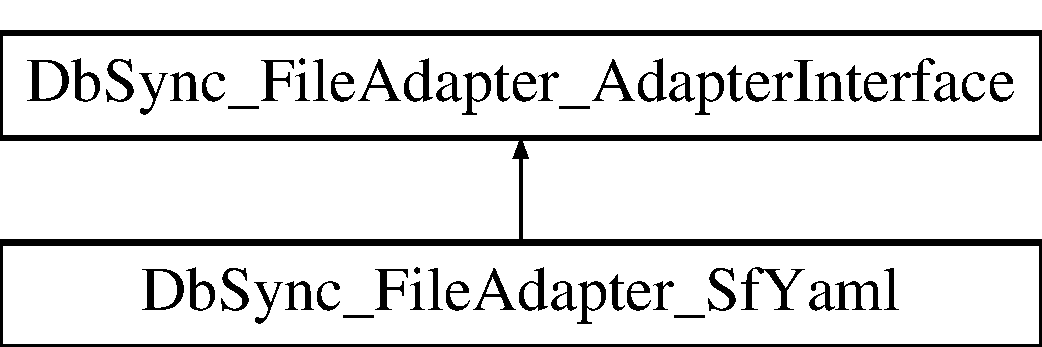
\includegraphics[height=2.000000cm]{interfaceDbSync__FileAdapter__AdapterInterface}
\end{center}
\end{figure}
\subsection*{Public Member Functions}
\begin{DoxyCompactItemize}
\item 
\hyperlink{interfaceDbSync__FileAdapter__AdapterInterface_abb3e223a99e5c0cd131c59acc6d82fc8}{\_\-\_\-construct} (\$path)
\item 
\hyperlink{interfaceDbSync__FileAdapter__AdapterInterface_a73ed1fa2cf12f3dc7f97981c4976b66b}{write} (\$filename, array \$data)
\item 
\hyperlink{interfaceDbSync__FileAdapter__AdapterInterface_a04bbebef17ee88c116b9ac67cc029f84}{load} (\$filename)
\item 
\hyperlink{interfaceDbSync__FileAdapter__AdapterInterface_a6a01ded2d94740261a4ff748bd900bf2}{getTableList} (\hyperlink{classDbSync__Model__AbstractModel}{DbSync\_\-Model\_\-AbstractModel} \$model)
\item 
\hyperlink{interfaceDbSync__FileAdapter__AdapterInterface_af99365b89b70a2be914b32bee7c73962}{getFilePath} (\hyperlink{classDbSync__Model__AbstractModel}{DbSync\_\-Model\_\-AbstractModel} \$model)
\item 
\hyperlink{interfaceDbSync__FileAdapter__AdapterInterface_a11acefe78ea2cf6693390d280ed98ab5}{getTableByTrigger} (\$triggerName)
\item 
\hyperlink{interfaceDbSync__FileAdapter__AdapterInterface_a3a1720dbec000385230a831e06ad8255}{getTriggerList} ()
\end{DoxyCompactItemize}


\subsection{Constructor \& Destructor Documentation}
\hypertarget{interfaceDbSync__FileAdapter__AdapterInterface_abb3e223a99e5c0cd131c59acc6d82fc8}{
\index{DbSync\_\-FileAdapter\_\-AdapterInterface@{DbSync\_\-FileAdapter\_\-AdapterInterface}!\_\-\_\-construct@{\_\-\_\-construct}}
\index{\_\-\_\-construct@{\_\-\_\-construct}!DbSync_FileAdapter_AdapterInterface@{DbSync\_\-FileAdapter\_\-AdapterInterface}}
\subsubsection[{\_\-\_\-construct}]{\setlength{\rightskip}{0pt plus 5cm}DbSync\_\-FileAdapter\_\-AdapterInterface::\_\-\_\-construct (
\begin{DoxyParamCaption}
\item[{\$}]{path}
\end{DoxyParamCaption}
)}}
\label{interfaceDbSync__FileAdapter__AdapterInterface_abb3e223a99e5c0cd131c59acc6d82fc8}
Contructor


\begin{DoxyParams}[1]{Parameters}
string & {\em \$path} & \\
\hline
\end{DoxyParams}


Implemented in \hyperlink{classDbSync__FileAdapter__SfYaml_acb7865b3fc2f34a6ae75403f6a88157b}{DbSync\_\-FileAdapter\_\-SfYaml}.



\subsection{Member Function Documentation}
\hypertarget{interfaceDbSync__FileAdapter__AdapterInterface_af99365b89b70a2be914b32bee7c73962}{
\index{DbSync\_\-FileAdapter\_\-AdapterInterface@{DbSync\_\-FileAdapter\_\-AdapterInterface}!getFilePath@{getFilePath}}
\index{getFilePath@{getFilePath}!DbSync_FileAdapter_AdapterInterface@{DbSync\_\-FileAdapter\_\-AdapterInterface}}
\subsubsection[{getFilePath}]{\setlength{\rightskip}{0pt plus 5cm}DbSync\_\-FileAdapter\_\-AdapterInterface::getFilePath (
\begin{DoxyParamCaption}
\item[{{\bf DbSync\_\-Model\_\-AbstractModel} \$}]{model}
\end{DoxyParamCaption}
)}}
\label{interfaceDbSync__FileAdapter__AdapterInterface_af99365b89b70a2be914b32bee7c73962}
Get config filepath


\begin{DoxyParams}[1]{Parameters}
\hyperlink{classDbSync__Model__AbstractModel}{DbSync\_\-Model\_\-AbstractModel} & {\em \$model} & \\
\hline
\end{DoxyParams}

\begin{DoxyExceptions}{Exceptions}
{\em Exception} & \\
\hline
\end{DoxyExceptions}
\begin{DoxyReturn}{Returns}
string 
\end{DoxyReturn}


Implemented in \hyperlink{classDbSync__FileAdapter__SfYaml_ae5e8cd6bf146147d55e5a28090c52d0d}{DbSync\_\-FileAdapter\_\-SfYaml}.

\hypertarget{interfaceDbSync__FileAdapter__AdapterInterface_a11acefe78ea2cf6693390d280ed98ab5}{
\index{DbSync\_\-FileAdapter\_\-AdapterInterface@{DbSync\_\-FileAdapter\_\-AdapterInterface}!getTableByTrigger@{getTableByTrigger}}
\index{getTableByTrigger@{getTableByTrigger}!DbSync_FileAdapter_AdapterInterface@{DbSync\_\-FileAdapter\_\-AdapterInterface}}
\subsubsection[{getTableByTrigger}]{\setlength{\rightskip}{0pt plus 5cm}DbSync\_\-FileAdapter\_\-AdapterInterface::getTableByTrigger (
\begin{DoxyParamCaption}
\item[{\$}]{triggerName}
\end{DoxyParamCaption}
)}}
\label{interfaceDbSync__FileAdapter__AdapterInterface_a11acefe78ea2cf6693390d280ed98ab5}
Get tableName by triggerName


\begin{DoxyParams}[1]{Parameters}
string & {\em \$triggerName} & \\
\hline
\end{DoxyParams}
\begin{DoxyReturn}{Returns}
string 
\end{DoxyReturn}


Implemented in \hyperlink{classDbSync__FileAdapter__SfYaml_a3f3f1ade545de6e0ccade4243f9e4819}{DbSync\_\-FileAdapter\_\-SfYaml}.

\hypertarget{interfaceDbSync__FileAdapter__AdapterInterface_a6a01ded2d94740261a4ff748bd900bf2}{
\index{DbSync\_\-FileAdapter\_\-AdapterInterface@{DbSync\_\-FileAdapter\_\-AdapterInterface}!getTableList@{getTableList}}
\index{getTableList@{getTableList}!DbSync_FileAdapter_AdapterInterface@{DbSync\_\-FileAdapter\_\-AdapterInterface}}
\subsubsection[{getTableList}]{\setlength{\rightskip}{0pt plus 5cm}DbSync\_\-FileAdapter\_\-AdapterInterface::getTableList (
\begin{DoxyParamCaption}
\item[{{\bf DbSync\_\-Model\_\-AbstractModel} \$}]{model}
\end{DoxyParamCaption}
)}}
\label{interfaceDbSync__FileAdapter__AdapterInterface_a6a01ded2d94740261a4ff748bd900bf2}
Get data tables list

\begin{DoxyReturn}{Returns}
array 
\end{DoxyReturn}


Implemented in \hyperlink{classDbSync__FileAdapter__SfYaml_a338a94760851e53949c22fe0454b0c7e}{DbSync\_\-FileAdapter\_\-SfYaml}.

\hypertarget{interfaceDbSync__FileAdapter__AdapterInterface_a3a1720dbec000385230a831e06ad8255}{
\index{DbSync\_\-FileAdapter\_\-AdapterInterface@{DbSync\_\-FileAdapter\_\-AdapterInterface}!getTriggerList@{getTriggerList}}
\index{getTriggerList@{getTriggerList}!DbSync_FileAdapter_AdapterInterface@{DbSync\_\-FileAdapter\_\-AdapterInterface}}
\subsubsection[{getTriggerList}]{\setlength{\rightskip}{0pt plus 5cm}DbSync\_\-FileAdapter\_\-AdapterInterface::getTriggerList (
\begin{DoxyParamCaption}
{}
\end{DoxyParamCaption}
)}}
\label{interfaceDbSync__FileAdapter__AdapterInterface_a3a1720dbec000385230a831e06ad8255}
Get triggers list

\begin{DoxyReturn}{Returns}
array 
\end{DoxyReturn}
\hypertarget{interfaceDbSync__FileAdapter__AdapterInterface_a04bbebef17ee88c116b9ac67cc029f84}{
\index{DbSync\_\-FileAdapter\_\-AdapterInterface@{DbSync\_\-FileAdapter\_\-AdapterInterface}!load@{load}}
\index{load@{load}!DbSync_FileAdapter_AdapterInterface@{DbSync\_\-FileAdapter\_\-AdapterInterface}}
\subsubsection[{load}]{\setlength{\rightskip}{0pt plus 5cm}DbSync\_\-FileAdapter\_\-AdapterInterface::load (
\begin{DoxyParamCaption}
\item[{\$}]{filename}
\end{DoxyParamCaption}
)}}
\label{interfaceDbSync__FileAdapter__AdapterInterface_a04bbebef17ee88c116b9ac67cc029f84}
Load data from file


\begin{DoxyParams}[1]{Parameters}
string & {\em \$filename} & \\
\hline
\end{DoxyParams}
\begin{DoxyReturn}{Returns}
array 
\end{DoxyReturn}


Implemented in \hyperlink{classDbSync__FileAdapter__SfYaml_a9a7bffcb73b3b66d27f265791dbfb44f}{DbSync\_\-FileAdapter\_\-SfYaml}.

\hypertarget{interfaceDbSync__FileAdapter__AdapterInterface_a73ed1fa2cf12f3dc7f97981c4976b66b}{
\index{DbSync\_\-FileAdapter\_\-AdapterInterface@{DbSync\_\-FileAdapter\_\-AdapterInterface}!write@{write}}
\index{write@{write}!DbSync_FileAdapter_AdapterInterface@{DbSync\_\-FileAdapter\_\-AdapterInterface}}
\subsubsection[{write}]{\setlength{\rightskip}{0pt plus 5cm}DbSync\_\-FileAdapter\_\-AdapterInterface::write (
\begin{DoxyParamCaption}
\item[{\$}]{filename, }
\item[{array \$}]{data}
\end{DoxyParamCaption}
)}}
\label{interfaceDbSync__FileAdapter__AdapterInterface_a73ed1fa2cf12f3dc7f97981c4976b66b}
Write data to file


\begin{DoxyParams}[1]{Parameters}
string & {\em \$filename} & Full path \\
\hline
array & {\em \$data} & \\
\hline
\end{DoxyParams}
\begin{DoxyReturn}{Returns}
int The function returns the number of bytes that were written to the file, or false on failure. 
\end{DoxyReturn}


Implemented in \hyperlink{classDbSync__FileAdapter__SfYaml_a186038cd277c53d0fd7512320dd8250a}{DbSync\_\-FileAdapter\_\-SfYaml}.



The documentation for this interface was generated from the following file:\begin{DoxyCompactItemize}
\item 
DbSync/FileAdapter/AdapterInterface.php\end{DoxyCompactItemize}

\hypertarget{classDbSync__FileAdapter__SfYaml}{
\section{DbSync\_\-FileAdapter\_\-SfYaml Class Reference}
\label{classDbSync__FileAdapter__SfYaml}\index{DbSync\_\-FileAdapter\_\-SfYaml@{DbSync\_\-FileAdapter\_\-SfYaml}}
}
Inheritance diagram for DbSync\_\-FileAdapter\_\-SfYaml:\begin{figure}[H]
\begin{center}
\leavevmode
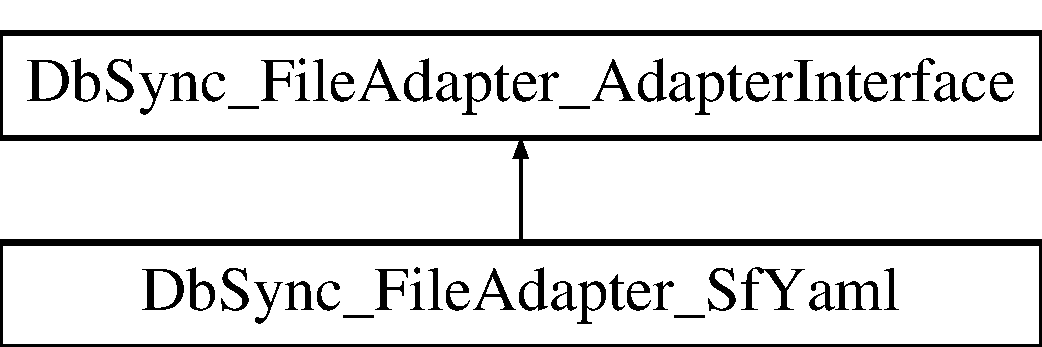
\includegraphics[height=2.000000cm]{classDbSync__FileAdapter__SfYaml}
\end{center}
\end{figure}
\subsection*{Public Member Functions}
\begin{DoxyCompactItemize}
\item 
\hyperlink{classDbSync__FileAdapter__SfYaml_acb7865b3fc2f34a6ae75403f6a88157b}{\_\-\_\-construct} (\$path)
\item 
\hyperlink{classDbSync__FileAdapter__SfYaml_a186038cd277c53d0fd7512320dd8250a}{write} (\$filename, array \$data)
\item 
\hyperlink{classDbSync__FileAdapter__SfYaml_a9a7bffcb73b3b66d27f265791dbfb44f}{load} (\$filename)
\item 
\hyperlink{classDbSync__FileAdapter__SfYaml_a338a94760851e53949c22fe0454b0c7e}{getTableList} (\hyperlink{classDbSync__Model__AbstractModel}{DbSync\_\-Model\_\-AbstractModel} \$model)
\item 
\hyperlink{classDbSync__FileAdapter__SfYaml_ae5e8cd6bf146147d55e5a28090c52d0d}{getFilePath} (\hyperlink{classDbSync__Model__AbstractModel}{DbSync\_\-Model\_\-AbstractModel} \$model)
\item 
\hyperlink{classDbSync__FileAdapter__SfYaml_a3f3f1ade545de6e0ccade4243f9e4819}{getTableByTrigger} (\$triggerName)
\item 
\hyperlink{classDbSync__FileAdapter__SfYaml_a99575fdc0db3410879efe12a8df4cf2c}{getTriggerList} (\$tables=array())
\item 
\hyperlink{classDbSync__FileAdapter__SfYaml_a56bd9eed9769e0b7122bad64e372acd6}{getIterator} (\$path, \$flags=FilesystemIterator::SKIP\_\-DOTS)
\end{DoxyCompactItemize}
\subsection*{Public Attributes}
\begin{DoxyCompactItemize}
\item 
\hypertarget{classDbSync__FileAdapter__SfYaml_a5f979fde3881a0d48322890061eecc00}{
const {\bfseries FILE\_\-EXTENSION} = 'yml'}
\label{classDbSync__FileAdapter__SfYaml_a5f979fde3881a0d48322890061eecc00}

\end{DoxyCompactItemize}
\subsection*{Protected Attributes}
\begin{DoxyCompactItemize}
\item 
\hypertarget{classDbSync__FileAdapter__SfYaml_a91b720068963d7b029c5b18334ad6091}{
{\bfseries \$\_\-path}}
\label{classDbSync__FileAdapter__SfYaml_a91b720068963d7b029c5b18334ad6091}

\end{DoxyCompactItemize}


\subsection{Constructor \& Destructor Documentation}
\hypertarget{classDbSync__FileAdapter__SfYaml_acb7865b3fc2f34a6ae75403f6a88157b}{
\index{DbSync\_\-FileAdapter\_\-SfYaml@{DbSync\_\-FileAdapter\_\-SfYaml}!\_\-\_\-construct@{\_\-\_\-construct}}
\index{\_\-\_\-construct@{\_\-\_\-construct}!DbSync_FileAdapter_SfYaml@{DbSync\_\-FileAdapter\_\-SfYaml}}
\subsubsection[{\_\-\_\-construct}]{\setlength{\rightskip}{0pt plus 5cm}DbSync\_\-FileAdapter\_\-SfYaml::\_\-\_\-construct (
\begin{DoxyParamCaption}
\item[{\$}]{path}
\end{DoxyParamCaption}
)}}
\label{classDbSync__FileAdapter__SfYaml_acb7865b3fc2f34a6ae75403f6a88157b}
Contructor


\begin{DoxyParams}[1]{Parameters}
string & {\em \$path} & \\
\hline
\end{DoxyParams}


Implements \hyperlink{interfaceDbSync__FileAdapter__AdapterInterface_abb3e223a99e5c0cd131c59acc6d82fc8}{DbSync\_\-FileAdapter\_\-AdapterInterface}.



\subsection{Member Function Documentation}
\hypertarget{classDbSync__FileAdapter__SfYaml_ae5e8cd6bf146147d55e5a28090c52d0d}{
\index{DbSync\_\-FileAdapter\_\-SfYaml@{DbSync\_\-FileAdapter\_\-SfYaml}!getFilePath@{getFilePath}}
\index{getFilePath@{getFilePath}!DbSync_FileAdapter_SfYaml@{DbSync\_\-FileAdapter\_\-SfYaml}}
\subsubsection[{getFilePath}]{\setlength{\rightskip}{0pt plus 5cm}DbSync\_\-FileAdapter\_\-SfYaml::getFilePath (
\begin{DoxyParamCaption}
\item[{{\bf DbSync\_\-Model\_\-AbstractModel} \$}]{model}
\end{DoxyParamCaption}
)}}
\label{classDbSync__FileAdapter__SfYaml_ae5e8cd6bf146147d55e5a28090c52d0d}
Get config filepath


\begin{DoxyParams}[1]{Parameters}
boolen & {\em \$real} & \\
\hline
\end{DoxyParams}

\begin{DoxyExceptions}{Exceptions}
{\em Exception} & \\
\hline
\end{DoxyExceptions}
\begin{DoxyReturn}{Returns}
string 
\end{DoxyReturn}


Implements \hyperlink{interfaceDbSync__FileAdapter__AdapterInterface_af99365b89b70a2be914b32bee7c73962}{DbSync\_\-FileAdapter\_\-AdapterInterface}.

\hypertarget{classDbSync__FileAdapter__SfYaml_a56bd9eed9769e0b7122bad64e372acd6}{
\index{DbSync\_\-FileAdapter\_\-SfYaml@{DbSync\_\-FileAdapter\_\-SfYaml}!getIterator@{getIterator}}
\index{getIterator@{getIterator}!DbSync_FileAdapter_SfYaml@{DbSync\_\-FileAdapter\_\-SfYaml}}
\subsubsection[{getIterator}]{\setlength{\rightskip}{0pt plus 5cm}DbSync\_\-FileAdapter\_\-SfYaml::getIterator (
\begin{DoxyParamCaption}
\item[{\$}]{path, }
\item[{\$}]{flags = {\ttfamily FilesystemIterator::SKIP\_\-DOTS}}
\end{DoxyParamCaption}
)}}
\label{classDbSync__FileAdapter__SfYaml_a56bd9eed9769e0b7122bad64e372acd6}
Get iterator


\begin{DoxyParams}[1]{Parameters}
string & {\em \$path} & \\
\hline
integer & {\em \$flags} & \\
\hline
\end{DoxyParams}
\begin{DoxyReturn}{Returns}
GlobIterator 
\end{DoxyReturn}
\hypertarget{classDbSync__FileAdapter__SfYaml_a3f3f1ade545de6e0ccade4243f9e4819}{
\index{DbSync\_\-FileAdapter\_\-SfYaml@{DbSync\_\-FileAdapter\_\-SfYaml}!getTableByTrigger@{getTableByTrigger}}
\index{getTableByTrigger@{getTableByTrigger}!DbSync_FileAdapter_SfYaml@{DbSync\_\-FileAdapter\_\-SfYaml}}
\subsubsection[{getTableByTrigger}]{\setlength{\rightskip}{0pt plus 5cm}DbSync\_\-FileAdapter\_\-SfYaml::getTableByTrigger (
\begin{DoxyParamCaption}
\item[{\$}]{triggerName}
\end{DoxyParamCaption}
)}}
\label{classDbSync__FileAdapter__SfYaml_a3f3f1ade545de6e0ccade4243f9e4819}
Get tableName by triggerName


\begin{DoxyParams}[1]{Parameters}
string & {\em \$triggerName} & \\
\hline
\end{DoxyParams}
\begin{DoxyReturn}{Returns}
string 
\end{DoxyReturn}


Implements \hyperlink{interfaceDbSync__FileAdapter__AdapterInterface_a11acefe78ea2cf6693390d280ed98ab5}{DbSync\_\-FileAdapter\_\-AdapterInterface}.

\hypertarget{classDbSync__FileAdapter__SfYaml_a338a94760851e53949c22fe0454b0c7e}{
\index{DbSync\_\-FileAdapter\_\-SfYaml@{DbSync\_\-FileAdapter\_\-SfYaml}!getTableList@{getTableList}}
\index{getTableList@{getTableList}!DbSync_FileAdapter_SfYaml@{DbSync\_\-FileAdapter\_\-SfYaml}}
\subsubsection[{getTableList}]{\setlength{\rightskip}{0pt plus 5cm}DbSync\_\-FileAdapter\_\-SfYaml::getTableList (
\begin{DoxyParamCaption}
\item[{{\bf DbSync\_\-Model\_\-AbstractModel} \$}]{model}
\end{DoxyParamCaption}
)}}
\label{classDbSync__FileAdapter__SfYaml_a338a94760851e53949c22fe0454b0c7e}
Get data tables list

\begin{DoxyReturn}{Returns}
array 
\end{DoxyReturn}


Implements \hyperlink{interfaceDbSync__FileAdapter__AdapterInterface_a6a01ded2d94740261a4ff748bd900bf2}{DbSync\_\-FileAdapter\_\-AdapterInterface}.

\hypertarget{classDbSync__FileAdapter__SfYaml_a99575fdc0db3410879efe12a8df4cf2c}{
\index{DbSync\_\-FileAdapter\_\-SfYaml@{DbSync\_\-FileAdapter\_\-SfYaml}!getTriggerList@{getTriggerList}}
\index{getTriggerList@{getTriggerList}!DbSync_FileAdapter_SfYaml@{DbSync\_\-FileAdapter\_\-SfYaml}}
\subsubsection[{getTriggerList}]{\setlength{\rightskip}{0pt plus 5cm}DbSync\_\-FileAdapter\_\-SfYaml::getTriggerList (
\begin{DoxyParamCaption}
\item[{\$}]{tables = {\ttfamily array()}}
\end{DoxyParamCaption}
)}}
\label{classDbSync__FileAdapter__SfYaml_a99575fdc0db3410879efe12a8df4cf2c}
Get triggers list


\begin{DoxyParams}[1]{Parameters}
array & {\em \$tables} & \\
\hline
\end{DoxyParams}
\begin{DoxyReturn}{Returns}
array 
\end{DoxyReturn}
\hypertarget{classDbSync__FileAdapter__SfYaml_a9a7bffcb73b3b66d27f265791dbfb44f}{
\index{DbSync\_\-FileAdapter\_\-SfYaml@{DbSync\_\-FileAdapter\_\-SfYaml}!load@{load}}
\index{load@{load}!DbSync_FileAdapter_SfYaml@{DbSync\_\-FileAdapter\_\-SfYaml}}
\subsubsection[{load}]{\setlength{\rightskip}{0pt plus 5cm}DbSync\_\-FileAdapter\_\-SfYaml::load (
\begin{DoxyParamCaption}
\item[{\$}]{filename}
\end{DoxyParamCaption}
)}}
\label{classDbSync__FileAdapter__SfYaml_a9a7bffcb73b3b66d27f265791dbfb44f}
Load data from file


\begin{DoxyParams}[1]{Parameters}
string & {\em \$filename} & \\
\hline
\end{DoxyParams}
\begin{DoxyReturn}{Returns}
array 
\end{DoxyReturn}


Implements \hyperlink{interfaceDbSync__FileAdapter__AdapterInterface_a04bbebef17ee88c116b9ac67cc029f84}{DbSync\_\-FileAdapter\_\-AdapterInterface}.

\hypertarget{classDbSync__FileAdapter__SfYaml_a186038cd277c53d0fd7512320dd8250a}{
\index{DbSync\_\-FileAdapter\_\-SfYaml@{DbSync\_\-FileAdapter\_\-SfYaml}!write@{write}}
\index{write@{write}!DbSync_FileAdapter_SfYaml@{DbSync\_\-FileAdapter\_\-SfYaml}}
\subsubsection[{write}]{\setlength{\rightskip}{0pt plus 5cm}DbSync\_\-FileAdapter\_\-SfYaml::write (
\begin{DoxyParamCaption}
\item[{\$}]{filename, }
\item[{array \$}]{data}
\end{DoxyParamCaption}
)}}
\label{classDbSync__FileAdapter__SfYaml_a186038cd277c53d0fd7512320dd8250a}
Write data to file


\begin{DoxyParams}[1]{Parameters}
string & {\em \$filename} & Full path \\
\hline
array & {\em \$data} & \\
\hline
\end{DoxyParams}
\begin{DoxyReturn}{Returns}
int The function returns the number of bytes that were written to the file, or false on failure. 
\end{DoxyReturn}


Implements \hyperlink{interfaceDbSync__FileAdapter__AdapterInterface_a73ed1fa2cf12f3dc7f97981c4976b66b}{DbSync\_\-FileAdapter\_\-AdapterInterface}.



The documentation for this class was generated from the following file:\begin{DoxyCompactItemize}
\item 
DbSync/FileAdapter/SfYaml.php\end{DoxyCompactItemize}

\hypertarget{classDbSync__Model__AbstractModel}{
\section{DbSync\_\-Model\_\-AbstractModel Class Reference}
\label{classDbSync__Model__AbstractModel}\index{DbSync\_\-Model\_\-AbstractModel@{DbSync\_\-Model\_\-AbstractModel}}
}
Inheritance diagram for DbSync\_\-Model\_\-AbstractModel:\begin{figure}[H]
\begin{center}
\leavevmode
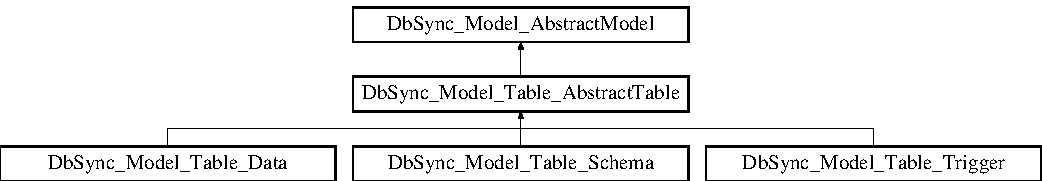
\includegraphics[height=2.434783cm]{classDbSync__Model__AbstractModel}
\end{center}
\end{figure}
\subsection*{Public Member Functions}
\begin{DoxyCompactItemize}
\item 
\hyperlink{classDbSync__Model__AbstractModel_a465d0b66eecc5bafe16c60a091818300}{\_\-\_\-construct} (\hyperlink{interfaceDbSync__DbAdapter__AdapterInterface}{DbSync\_\-DbAdapter\_\-AdapterInterface} \$db, \hyperlink{interfaceDbSync__FileAdapter__AdapterInterface}{DbSync\_\-FileAdapter\_\-AdapterInterface} \$file, \$diffProg=null)
\item 
\hyperlink{classDbSync__Model__AbstractModel_a3e74113d284bb77851210687c81132f0}{setDiffProg} (\$diffProg)
\item 
\hyperlink{classDbSync__Model__AbstractModel_a96803106cf4d9cd9397b36d51f968d48}{getName} ()
\item 
\hyperlink{classDbSync__Model__AbstractModel_aefc6efadc58c0252f5b40aaf1dd6ca3e}{save} (\$filename)
\item 
\hyperlink{classDbSync__Model__AbstractModel_a7c06c50106b8d6ed078a0c418daad2f6}{isWriteable} ()
\item 
\hyperlink{classDbSync__Model__AbstractModel_af11e8e35d3bf6119f2954836b844c5e4}{getFilePath} (\$real=true)
\item 
\hyperlink{classDbSync__Model__AbstractModel_ad2e2053df76dca54927230109adadb32}{hasFile} ()
\item 
\hyperlink{classDbSync__Model__AbstractModel_ad3165926fb191710d68d987548bc377a}{deleteFile} ()
\item 
\hyperlink{classDbSync__Model__AbstractModel_a2bde0fab39d14e31f2fb38c3401ac092}{getStatus} ()
\item 
\hyperlink{classDbSync__Model__AbstractModel_aa31931e01689ce7f5841a8fb268a753c}{pull} ()
\item 
\hyperlink{classDbSync__Model__AbstractModel_a93a3912dbc5e1667fde4dea420e36470}{push} ()
\item 
\hyperlink{classDbSync__Model__AbstractModel_aa340f69f9ed1f60df7238bc971db6489}{diff} ()
\item 
\hyperlink{classDbSync__Model__AbstractModel_a6dc082b13e12f68902dd659bc38c8865}{init} (\$force=false)
\end{DoxyCompactItemize}
\subsection*{Protected Attributes}
\begin{DoxyCompactItemize}
\item 
\hypertarget{classDbSync__Model__AbstractModel_a2c382721c637e9e8e1255f30cd63a1c7}{
{\bfseries \$\_\-dbAdapter}}
\label{classDbSync__Model__AbstractModel_a2c382721c637e9e8e1255f30cd63a1c7}

\item 
\hypertarget{classDbSync__Model__AbstractModel_aaa04c006f050eab22fed7403eddc7683}{
{\bfseries \$\_\-fileAdapter}}
\label{classDbSync__Model__AbstractModel_aaa04c006f050eab22fed7403eddc7683}

\item 
\hypertarget{classDbSync__Model__AbstractModel_a9a61531b7ae157f0d61e04e3e139f761}{
{\bfseries \$\_\-diff} = 'diff'}
\label{classDbSync__Model__AbstractModel_a9a61531b7ae157f0d61e04e3e139f761}

\item 
\hypertarget{classDbSync__Model__AbstractModel_afc456aa77dbba891beec93ca092d1a0a}{
{\bfseries \$\_\-exceptionClass} = '\hyperlink{classDbSync__Exception}{DbSync\_\-Exception}'}
\label{classDbSync__Model__AbstractModel_afc456aa77dbba891beec93ca092d1a0a}

\end{DoxyCompactItemize}


\subsection{Constructor \& Destructor Documentation}
\hypertarget{classDbSync__Model__AbstractModel_a465d0b66eecc5bafe16c60a091818300}{
\index{DbSync\_\-Model\_\-AbstractModel@{DbSync\_\-Model\_\-AbstractModel}!\_\-\_\-construct@{\_\-\_\-construct}}
\index{\_\-\_\-construct@{\_\-\_\-construct}!DbSync_Model_AbstractModel@{DbSync\_\-Model\_\-AbstractModel}}
\subsubsection[{\_\-\_\-construct}]{\setlength{\rightskip}{0pt plus 5cm}DbSync\_\-Model\_\-AbstractModel::\_\-\_\-construct (
\begin{DoxyParamCaption}
\item[{{\bf DbSync\_\-DbAdapter\_\-AdapterInterface} \$}]{db, }
\item[{{\bf DbSync\_\-FileAdapter\_\-AdapterInterface} \$}]{file, }
\item[{\$}]{diffProg = {\ttfamily null}}
\end{DoxyParamCaption}
)}}
\label{classDbSync__Model__AbstractModel_a465d0b66eecc5bafe16c60a091818300}
Constructor


\begin{DoxyParams}[1]{Parameters}
\hyperlink{interfaceDbSync__DbAdapter__AdapterInterface}{DbSync\_\-DbAdapter\_\-AdapterInterface} & {\em \$db} & \\
\hline
\hyperlink{interfaceDbSync__FileAdapter__AdapterInterface}{DbSync\_\-FileAdapter\_\-AdapterInterface} & {\em \$file} & \\
\hline
string & {\em \$diffProg} & \\
\hline
\end{DoxyParams}


\subsection{Member Function Documentation}
\hypertarget{classDbSync__Model__AbstractModel_ad3165926fb191710d68d987548bc377a}{
\index{DbSync\_\-Model\_\-AbstractModel@{DbSync\_\-Model\_\-AbstractModel}!deleteFile@{deleteFile}}
\index{deleteFile@{deleteFile}!DbSync_Model_AbstractModel@{DbSync\_\-Model\_\-AbstractModel}}
\subsubsection[{deleteFile}]{\setlength{\rightskip}{0pt plus 5cm}DbSync\_\-Model\_\-AbstractModel::deleteFile (
\begin{DoxyParamCaption}
{}
\end{DoxyParamCaption}
)}}
\label{classDbSync__Model__AbstractModel_ad3165926fb191710d68d987548bc377a}
Delete file


\begin{DoxyExceptions}{Exceptions}
{\em \hyperlink{classDbSync__Exception}{DbSync\_\-Exception}} & \\
\hline
\end{DoxyExceptions}
\begin{DoxyReturn}{Returns}
boolen 
\end{DoxyReturn}
\hypertarget{classDbSync__Model__AbstractModel_aa340f69f9ed1f60df7238bc971db6489}{
\index{DbSync\_\-Model\_\-AbstractModel@{DbSync\_\-Model\_\-AbstractModel}!diff@{diff}}
\index{diff@{diff}!DbSync_Model_AbstractModel@{DbSync\_\-Model\_\-AbstractModel}}
\subsubsection[{diff}]{\setlength{\rightskip}{0pt plus 5cm}DbSync\_\-Model\_\-AbstractModel::diff (
\begin{DoxyParamCaption}
{}
\end{DoxyParamCaption}
)}}
\label{classDbSync__Model__AbstractModel_aa340f69f9ed1f60df7238bc971db6489}
Get diff

\begin{DoxyReturn}{Returns}
array 
\end{DoxyReturn}

\begin{DoxyExceptions}{Exceptions}
{\em \hyperlink{classDbSync__Exception}{DbSync\_\-Exception}} & \\
\hline
\end{DoxyExceptions}
\hypertarget{classDbSync__Model__AbstractModel_af11e8e35d3bf6119f2954836b844c5e4}{
\index{DbSync\_\-Model\_\-AbstractModel@{DbSync\_\-Model\_\-AbstractModel}!getFilePath@{getFilePath}}
\index{getFilePath@{getFilePath}!DbSync_Model_AbstractModel@{DbSync\_\-Model\_\-AbstractModel}}
\subsubsection[{getFilePath}]{\setlength{\rightskip}{0pt plus 5cm}DbSync\_\-Model\_\-AbstractModel::getFilePath (
\begin{DoxyParamCaption}
\item[{\$}]{real = {\ttfamily true}}
\end{DoxyParamCaption}
)}}
\label{classDbSync__Model__AbstractModel_af11e8e35d3bf6119f2954836b844c5e4}
Get config filepath


\begin{DoxyParams}[1]{Parameters}
boolen & {\em \$real} & \\
\hline
\end{DoxyParams}
\begin{DoxyReturn}{Returns}
string 
\end{DoxyReturn}
\hypertarget{classDbSync__Model__AbstractModel_a96803106cf4d9cd9397b36d51f968d48}{
\index{DbSync\_\-Model\_\-AbstractModel@{DbSync\_\-Model\_\-AbstractModel}!getName@{getName}}
\index{getName@{getName}!DbSync_Model_AbstractModel@{DbSync\_\-Model\_\-AbstractModel}}
\subsubsection[{getName}]{\setlength{\rightskip}{0pt plus 5cm}DbSync\_\-Model\_\-AbstractModel::getName (
\begin{DoxyParamCaption}
{}
\end{DoxyParamCaption}
)\hspace{0.3cm}{\ttfamily  \mbox{[}abstract\mbox{]}}}}
\label{classDbSync__Model__AbstractModel_a96803106cf4d9cd9397b36d51f968d48}
Get item name

\begin{DoxyReturn}{Returns}
string 
\end{DoxyReturn}


Reimplemented in \hyperlink{classDbSync__Model__Table__AbstractTable_a88726b043a43248114ca3e3faa9025d2}{DbSync\_\-Model\_\-Table\_\-AbstractTable}, and \hyperlink{classDbSync__Model__Table__Trigger_a82965dc7d44b8c3722b4830c6c7cc7ea}{DbSync\_\-Model\_\-Table\_\-Trigger}.

\hypertarget{classDbSync__Model__AbstractModel_a2bde0fab39d14e31f2fb38c3401ac092}{
\index{DbSync\_\-Model\_\-AbstractModel@{DbSync\_\-Model\_\-AbstractModel}!getStatus@{getStatus}}
\index{getStatus@{getStatus}!DbSync_Model_AbstractModel@{DbSync\_\-Model\_\-AbstractModel}}
\subsubsection[{getStatus}]{\setlength{\rightskip}{0pt plus 5cm}DbSync\_\-Model\_\-AbstractModel::getStatus (
\begin{DoxyParamCaption}
{}
\end{DoxyParamCaption}
)}}
\label{classDbSync__Model__AbstractModel_a2bde0fab39d14e31f2fb38c3401ac092}
Get status

\begin{DoxyReturn}{Returns}
boolen 
\end{DoxyReturn}
\hypertarget{classDbSync__Model__AbstractModel_ad2e2053df76dca54927230109adadb32}{
\index{DbSync\_\-Model\_\-AbstractModel@{DbSync\_\-Model\_\-AbstractModel}!hasFile@{hasFile}}
\index{hasFile@{hasFile}!DbSync_Model_AbstractModel@{DbSync\_\-Model\_\-AbstractModel}}
\subsubsection[{hasFile}]{\setlength{\rightskip}{0pt plus 5cm}DbSync\_\-Model\_\-AbstractModel::hasFile (
\begin{DoxyParamCaption}
{}
\end{DoxyParamCaption}
)}}
\label{classDbSync__Model__AbstractModel_ad2e2053df76dca54927230109adadb32}
Has file

\begin{DoxyReturn}{Returns}
boolen 
\end{DoxyReturn}
\hypertarget{classDbSync__Model__AbstractModel_a6dc082b13e12f68902dd659bc38c8865}{
\index{DbSync\_\-Model\_\-AbstractModel@{DbSync\_\-Model\_\-AbstractModel}!init@{init}}
\index{init@{init}!DbSync_Model_AbstractModel@{DbSync\_\-Model\_\-AbstractModel}}
\subsubsection[{init}]{\setlength{\rightskip}{0pt plus 5cm}DbSync\_\-Model\_\-AbstractModel::init (
\begin{DoxyParamCaption}
\item[{\$}]{force = {\ttfamily false}}
\end{DoxyParamCaption}
)}}
\label{classDbSync__Model__AbstractModel_a6dc082b13e12f68902dd659bc38c8865}
Init


\begin{DoxyParams}[1]{Parameters}
boolen & {\em \$force} & \\
\hline
\end{DoxyParams}

\begin{DoxyExceptions}{Exceptions}
{\em \hyperlink{classDbSync__Exception}{DbSync\_\-Exception}} & \\
\hline
\end{DoxyExceptions}
\begin{DoxyReturn}{Returns}
boolean 
\end{DoxyReturn}
\hypertarget{classDbSync__Model__AbstractModel_a7c06c50106b8d6ed078a0c418daad2f6}{
\index{DbSync\_\-Model\_\-AbstractModel@{DbSync\_\-Model\_\-AbstractModel}!isWriteable@{isWriteable}}
\index{isWriteable@{isWriteable}!DbSync_Model_AbstractModel@{DbSync\_\-Model\_\-AbstractModel}}
\subsubsection[{isWriteable}]{\setlength{\rightskip}{0pt plus 5cm}DbSync\_\-Model\_\-AbstractModel::isWriteable (
\begin{DoxyParamCaption}
{}
\end{DoxyParamCaption}
)}}
\label{classDbSync__Model__AbstractModel_a7c06c50106b8d6ed078a0c418daad2f6}
Is directory writable

\begin{DoxyReturn}{Returns}
boolean 
\end{DoxyReturn}
\hypertarget{classDbSync__Model__AbstractModel_aa31931e01689ce7f5841a8fb268a753c}{
\index{DbSync\_\-Model\_\-AbstractModel@{DbSync\_\-Model\_\-AbstractModel}!pull@{pull}}
\index{pull@{pull}!DbSync_Model_AbstractModel@{DbSync\_\-Model\_\-AbstractModel}}
\subsubsection[{pull}]{\setlength{\rightskip}{0pt plus 5cm}DbSync\_\-Model\_\-AbstractModel::pull (
\begin{DoxyParamCaption}
{}
\end{DoxyParamCaption}
)}}
\label{classDbSync__Model__AbstractModel_aa31931e01689ce7f5841a8fb268a753c}
Pull schema or data from db table to config file \hypertarget{classDbSync__Model__AbstractModel_a93a3912dbc5e1667fde4dea420e36470}{
\index{DbSync\_\-Model\_\-AbstractModel@{DbSync\_\-Model\_\-AbstractModel}!push@{push}}
\index{push@{push}!DbSync_Model_AbstractModel@{DbSync\_\-Model\_\-AbstractModel}}
\subsubsection[{push}]{\setlength{\rightskip}{0pt plus 5cm}DbSync\_\-Model\_\-AbstractModel::push (
\begin{DoxyParamCaption}
{}
\end{DoxyParamCaption}
)}}
\label{classDbSync__Model__AbstractModel_a93a3912dbc5e1667fde4dea420e36470}
Alter db table

\begin{DoxyReturn}{Returns}
boolen 
\end{DoxyReturn}
\hypertarget{classDbSync__Model__AbstractModel_aefc6efadc58c0252f5b40aaf1dd6ca3e}{
\index{DbSync\_\-Model\_\-AbstractModel@{DbSync\_\-Model\_\-AbstractModel}!save@{save}}
\index{save@{save}!DbSync_Model_AbstractModel@{DbSync\_\-Model\_\-AbstractModel}}
\subsubsection[{save}]{\setlength{\rightskip}{0pt plus 5cm}DbSync\_\-Model\_\-AbstractModel::save (
\begin{DoxyParamCaption}
\item[{\$}]{filename}
\end{DoxyParamCaption}
)}}
\label{classDbSync__Model__AbstractModel_aefc6efadc58c0252f5b40aaf1dd6ca3e}
Save config file


\begin{DoxyParams}[1]{Parameters}
string & {\em \$filename} & \\
\hline
\end{DoxyParams}

\begin{DoxyExceptions}{Exceptions}
{\em \hyperlink{classDbSync__Exception}{DbSync\_\-Exception}} & \\
\hline
\end{DoxyExceptions}
\hypertarget{classDbSync__Model__AbstractModel_a3e74113d284bb77851210687c81132f0}{
\index{DbSync\_\-Model\_\-AbstractModel@{DbSync\_\-Model\_\-AbstractModel}!setDiffProg@{setDiffProg}}
\index{setDiffProg@{setDiffProg}!DbSync_Model_AbstractModel@{DbSync\_\-Model\_\-AbstractModel}}
\subsubsection[{setDiffProg}]{\setlength{\rightskip}{0pt plus 5cm}DbSync\_\-Model\_\-AbstractModel::setDiffProg (
\begin{DoxyParamCaption}
\item[{\$}]{diffProg}
\end{DoxyParamCaption}
)}}
\label{classDbSync__Model__AbstractModel_a3e74113d284bb77851210687c81132f0}
Set diff programm


\begin{DoxyParams}[1]{Parameters}
string & {\em \$diffProg} & \\
\hline
\end{DoxyParams}
\begin{DoxyReturn}{Returns}
\hyperlink{classDbSync__Model__AbstractModel}{DbSync\_\-Model\_\-AbstractModel} 
\end{DoxyReturn}


The documentation for this class was generated from the following file:\begin{DoxyCompactItemize}
\item 
DbSync/Model/AbstractModel.php\end{DoxyCompactItemize}

\hypertarget{classDbSync__Model__Table__AbstractTable}{
\section{DbSync\_\-Model\_\-Table\_\-AbstractTable Class Reference}
\label{classDbSync__Model__Table__AbstractTable}\index{DbSync\_\-Model\_\-Table\_\-AbstractTable@{DbSync\_\-Model\_\-Table\_\-AbstractTable}}
}
Inheritance diagram for DbSync\_\-Model\_\-Table\_\-AbstractTable:\begin{figure}[H]
\begin{center}
\leavevmode
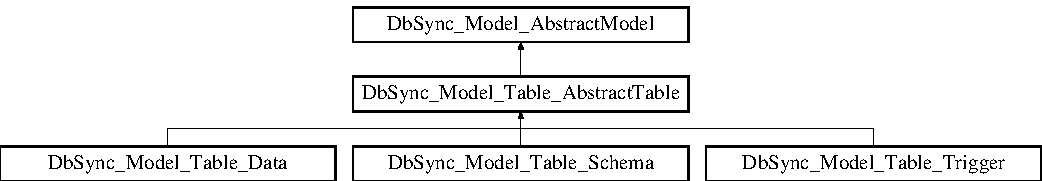
\includegraphics[height=2.434783cm]{classDbSync__Model__Table__AbstractTable}
\end{center}
\end{figure}
\subsection*{Public Member Functions}
\begin{DoxyCompactItemize}
\item 
\hyperlink{classDbSync__Model__Table__AbstractTable_a8ee4b6ffc0539b45a791bc04eebe7548}{getTableName} ()
\item 
\hyperlink{classDbSync__Model__Table__AbstractTable_a88726b043a43248114ca3e3faa9025d2}{getName} ()
\item 
\hyperlink{classDbSync__Model__Table__AbstractTable_ab72bd2fe433d9ccd5d7e0d0451cc839a}{setTableName} (\$tableName)
\item 
\hyperlink{classDbSync__Model__Table__AbstractTable_abd2ae2adced70abce42204784c057253}{getListDb} ()
\item 
\hyperlink{classDbSync__Model__Table__AbstractTable_ae8ca43e4679f1fd0740ab4dde780609d}{getListConfig} ()
\item 
\hyperlink{classDbSync__Model__Table__AbstractTable_ac9ef882ae4805c341c228290b27ebc2d}{getList} ()
\item 
\hyperlink{classDbSync__Model__Table__AbstractTable_a4823777422da6c8522fac76402e307cd}{hasDbTable} ()
\end{DoxyCompactItemize}
\subsection*{Protected Attributes}
\begin{DoxyCompactItemize}
\item 
\hypertarget{classDbSync__Model__Table__AbstractTable_af53e7af896d208be81a6042724321026}{
{\bfseries \$\_\-tableName}}
\label{classDbSync__Model__Table__AbstractTable_af53e7af896d208be81a6042724321026}

\end{DoxyCompactItemize}


\subsection{Member Function Documentation}
\hypertarget{classDbSync__Model__Table__AbstractTable_ac9ef882ae4805c341c228290b27ebc2d}{
\index{DbSync\_\-Model\_\-Table\_\-AbstractTable@{DbSync\_\-Model\_\-Table\_\-AbstractTable}!getList@{getList}}
\index{getList@{getList}!DbSync_Model_Table_AbstractTable@{DbSync\_\-Model\_\-Table\_\-AbstractTable}}
\subsubsection[{getList}]{\setlength{\rightskip}{0pt plus 5cm}DbSync\_\-Model\_\-Table\_\-AbstractTable::getList (
\begin{DoxyParamCaption}
{}
\end{DoxyParamCaption}
)}}
\label{classDbSync__Model__Table__AbstractTable_ac9ef882ae4805c341c228290b27ebc2d}
Get list

\begin{DoxyReturn}{Returns}
array 
\end{DoxyReturn}
\hypertarget{classDbSync__Model__Table__AbstractTable_ae8ca43e4679f1fd0740ab4dde780609d}{
\index{DbSync\_\-Model\_\-Table\_\-AbstractTable@{DbSync\_\-Model\_\-Table\_\-AbstractTable}!getListConfig@{getListConfig}}
\index{getListConfig@{getListConfig}!DbSync_Model_Table_AbstractTable@{DbSync\_\-Model\_\-Table\_\-AbstractTable}}
\subsubsection[{getListConfig}]{\setlength{\rightskip}{0pt plus 5cm}DbSync\_\-Model\_\-Table\_\-AbstractTable::getListConfig (
\begin{DoxyParamCaption}
{}
\end{DoxyParamCaption}
)}}
\label{classDbSync__Model__Table__AbstractTable_ae8ca43e4679f1fd0740ab4dde780609d}
Get config tables list

\begin{DoxyReturn}{Returns}
array 
\end{DoxyReturn}
\hypertarget{classDbSync__Model__Table__AbstractTable_abd2ae2adced70abce42204784c057253}{
\index{DbSync\_\-Model\_\-Table\_\-AbstractTable@{DbSync\_\-Model\_\-Table\_\-AbstractTable}!getListDb@{getListDb}}
\index{getListDb@{getListDb}!DbSync_Model_Table_AbstractTable@{DbSync\_\-Model\_\-Table\_\-AbstractTable}}
\subsubsection[{getListDb}]{\setlength{\rightskip}{0pt plus 5cm}DbSync\_\-Model\_\-Table\_\-AbstractTable::getListDb (
\begin{DoxyParamCaption}
{}
\end{DoxyParamCaption}
)}}
\label{classDbSync__Model__Table__AbstractTable_abd2ae2adced70abce42204784c057253}
Get db tables list

\begin{DoxyReturn}{Returns}
array 
\end{DoxyReturn}
\hypertarget{classDbSync__Model__Table__AbstractTable_a88726b043a43248114ca3e3faa9025d2}{
\index{DbSync\_\-Model\_\-Table\_\-AbstractTable@{DbSync\_\-Model\_\-Table\_\-AbstractTable}!getName@{getName}}
\index{getName@{getName}!DbSync_Model_Table_AbstractTable@{DbSync\_\-Model\_\-Table\_\-AbstractTable}}
\subsubsection[{getName}]{\setlength{\rightskip}{0pt plus 5cm}DbSync\_\-Model\_\-Table\_\-AbstractTable::getName (
\begin{DoxyParamCaption}
{}
\end{DoxyParamCaption}
)}}
\label{classDbSync__Model__Table__AbstractTable_a88726b043a43248114ca3e3faa9025d2}
Get name

\begin{DoxyReturn}{Returns}
string 
\end{DoxyReturn}


Reimplemented from \hyperlink{classDbSync__Model__AbstractModel_a96803106cf4d9cd9397b36d51f968d48}{DbSync\_\-Model\_\-AbstractModel}.



Reimplemented in \hyperlink{classDbSync__Model__Table__Trigger_a82965dc7d44b8c3722b4830c6c7cc7ea}{DbSync\_\-Model\_\-Table\_\-Trigger}.

\hypertarget{classDbSync__Model__Table__AbstractTable_a8ee4b6ffc0539b45a791bc04eebe7548}{
\index{DbSync\_\-Model\_\-Table\_\-AbstractTable@{DbSync\_\-Model\_\-Table\_\-AbstractTable}!getTableName@{getTableName}}
\index{getTableName@{getTableName}!DbSync_Model_Table_AbstractTable@{DbSync\_\-Model\_\-Table\_\-AbstractTable}}
\subsubsection[{getTableName}]{\setlength{\rightskip}{0pt plus 5cm}DbSync\_\-Model\_\-Table\_\-AbstractTable::getTableName (
\begin{DoxyParamCaption}
{}
\end{DoxyParamCaption}
)}}
\label{classDbSync__Model__Table__AbstractTable_a8ee4b6ffc0539b45a791bc04eebe7548}
Get table name

\begin{DoxyReturn}{Returns}
string 
\end{DoxyReturn}

\begin{DoxyExceptions}{Exceptions}
{\em \hyperlink{classDbSync__Exception}{DbSync\_\-Exception}} & \\
\hline
\end{DoxyExceptions}


Reimplemented in \hyperlink{classDbSync__Model__Table__Trigger_a8b13bee47b742b987a07533dba66da76}{DbSync\_\-Model\_\-Table\_\-Trigger}.

\hypertarget{classDbSync__Model__Table__AbstractTable_a4823777422da6c8522fac76402e307cd}{
\index{DbSync\_\-Model\_\-Table\_\-AbstractTable@{DbSync\_\-Model\_\-Table\_\-AbstractTable}!hasDbTable@{hasDbTable}}
\index{hasDbTable@{hasDbTable}!DbSync_Model_Table_AbstractTable@{DbSync\_\-Model\_\-Table\_\-AbstractTable}}
\subsubsection[{hasDbTable}]{\setlength{\rightskip}{0pt plus 5cm}DbSync\_\-Model\_\-Table\_\-AbstractTable::hasDbTable (
\begin{DoxyParamCaption}
{}
\end{DoxyParamCaption}
)}}
\label{classDbSync__Model__Table__AbstractTable_a4823777422da6c8522fac76402e307cd}
Is db table exists

\begin{DoxyReturn}{Returns}
boolen 
\end{DoxyReturn}
\hypertarget{classDbSync__Model__Table__AbstractTable_ab72bd2fe433d9ccd5d7e0d0451cc839a}{
\index{DbSync\_\-Model\_\-Table\_\-AbstractTable@{DbSync\_\-Model\_\-Table\_\-AbstractTable}!setTableName@{setTableName}}
\index{setTableName@{setTableName}!DbSync_Model_Table_AbstractTable@{DbSync\_\-Model\_\-Table\_\-AbstractTable}}
\subsubsection[{setTableName}]{\setlength{\rightskip}{0pt plus 5cm}DbSync\_\-Model\_\-Table\_\-AbstractTable::setTableName (
\begin{DoxyParamCaption}
\item[{\$}]{tableName}
\end{DoxyParamCaption}
)}}
\label{classDbSync__Model__Table__AbstractTable_ab72bd2fe433d9ccd5d7e0d0451cc839a}
Set table name


\begin{DoxyParams}[1]{Parameters}
string & {\em \$tableName} & \\
\hline
\end{DoxyParams}
\begin{DoxyReturn}{Returns}
\hyperlink{classDbSync__Model__Table__AbstractTable}{DbSync\_\-Model\_\-Table\_\-AbstractTable} 
\end{DoxyReturn}


The documentation for this class was generated from the following file:\begin{DoxyCompactItemize}
\item 
DbSync/Model/Table/AbstractTable.php\end{DoxyCompactItemize}

\hypertarget{classDbSync__Model__Table__Data}{
\section{DbSync\_\-Model\_\-Table\_\-Data Class Reference}
\label{classDbSync__Model__Table__Data}\index{DbSync\_\-Model\_\-Table\_\-Data@{DbSync\_\-Model\_\-Table\_\-Data}}
}
Inheritance diagram for DbSync\_\-Model\_\-Table\_\-Data:\begin{figure}[H]
\begin{center}
\leavevmode
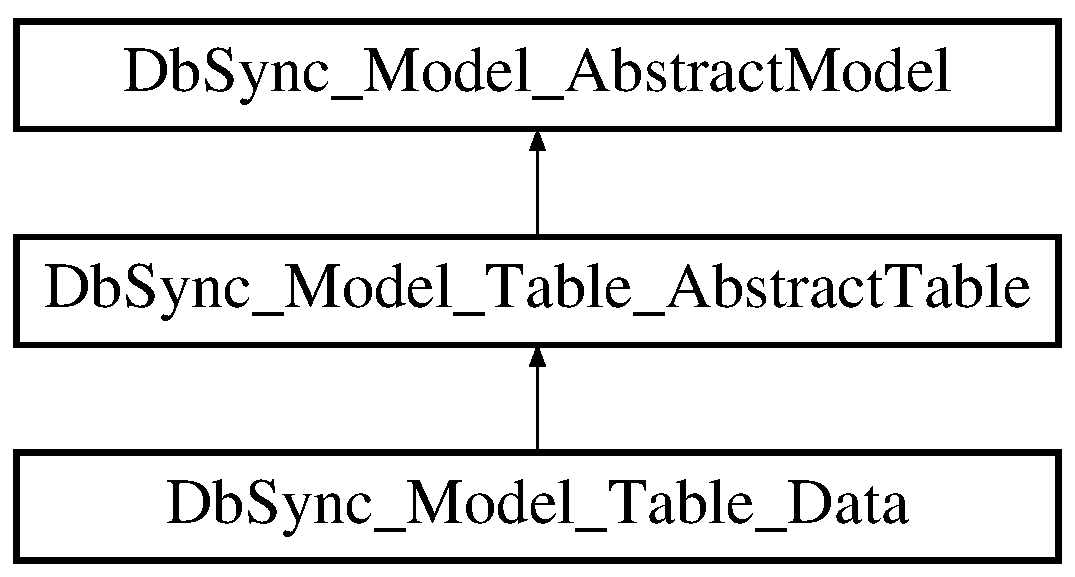
\includegraphics[height=3.000000cm]{classDbSync__Model__Table__Data}
\end{center}
\end{figure}
\subsection*{Public Member Functions}
\begin{DoxyCompactItemize}
\item 
\hyperlink{classDbSync__Model__Table__Data_a8476edd65b932c52fab20345b40170be}{generateConfigData} ()
\item 
\hyperlink{classDbSync__Model__Table__Data_a8da434a0d1eac198c3a327d48901b7d0}{push} (\$type=null)
\item 
\hyperlink{classDbSync__Model__Table__Data_a4158723195a0172984d176d28055c332}{isEmptyTable} ()
\end{DoxyCompactItemize}
\subsection*{Public Attributes}
\begin{DoxyCompactItemize}
\item 
\hypertarget{classDbSync__Model__Table__Data_a97aad1ea1d7d55a934e821fb5e7858d4}{
const {\bfseries PUSH\_\-TYPE\_\-FORCE} = 1}
\label{classDbSync__Model__Table__Data_a97aad1ea1d7d55a934e821fb5e7858d4}

\item 
\hypertarget{classDbSync__Model__Table__Data_acfe1e2aaa5f3256fddadf6034b5cfd67}{
const {\bfseries PUSH\_\-TYPE\_\-MERGE} = 2}
\label{classDbSync__Model__Table__Data_acfe1e2aaa5f3256fddadf6034b5cfd67}

\end{DoxyCompactItemize}


\subsection{Member Function Documentation}
\hypertarget{classDbSync__Model__Table__Data_a8476edd65b932c52fab20345b40170be}{
\index{DbSync\_\-Model\_\-Table\_\-Data@{DbSync\_\-Model\_\-Table\_\-Data}!generateConfigData@{generateConfigData}}
\index{generateConfigData@{generateConfigData}!DbSync_Model_Table_Data@{DbSync\_\-Model\_\-Table\_\-Data}}
\subsubsection[{generateConfigData}]{\setlength{\rightskip}{0pt plus 5cm}DbSync\_\-Model\_\-Table\_\-Data::generateConfigData (
\begin{DoxyParamCaption}
{}
\end{DoxyParamCaption}
)}}
\label{classDbSync__Model__Table__Data_a8476edd65b932c52fab20345b40170be}
Get data to store in config file

\begin{DoxyReturn}{Returns}
array 
\end{DoxyReturn}
\hypertarget{classDbSync__Model__Table__Data_a4158723195a0172984d176d28055c332}{
\index{DbSync\_\-Model\_\-Table\_\-Data@{DbSync\_\-Model\_\-Table\_\-Data}!isEmptyTable@{isEmptyTable}}
\index{isEmptyTable@{isEmptyTable}!DbSync_Model_Table_Data@{DbSync\_\-Model\_\-Table\_\-Data}}
\subsubsection[{isEmptyTable}]{\setlength{\rightskip}{0pt plus 5cm}DbSync\_\-Model\_\-Table\_\-Data::isEmptyTable (
\begin{DoxyParamCaption}
{}
\end{DoxyParamCaption}
)}}
\label{classDbSync__Model__Table__Data_a4158723195a0172984d176d28055c332}
Is db table dirty

\begin{DoxyReturn}{Returns}
boolean 
\end{DoxyReturn}

\begin{DoxyExceptions}{Exceptions}
{\em \hyperlink{classDbSync__Exception}{DbSync\_\-Exception}} & \\
\hline
\end{DoxyExceptions}
\hypertarget{classDbSync__Model__Table__Data_a8da434a0d1eac198c3a327d48901b7d0}{
\index{DbSync\_\-Model\_\-Table\_\-Data@{DbSync\_\-Model\_\-Table\_\-Data}!push@{push}}
\index{push@{push}!DbSync_Model_Table_Data@{DbSync\_\-Model\_\-Table\_\-Data}}
\subsubsection[{push}]{\setlength{\rightskip}{0pt plus 5cm}DbSync\_\-Model\_\-Table\_\-Data::push (
\begin{DoxyParamCaption}
\item[{\$}]{type = {\ttfamily null}}
\end{DoxyParamCaption}
)}}
\label{classDbSync__Model__Table__Data_a8da434a0d1eac198c3a327d48901b7d0}
Push data to db table


\begin{DoxyParams}[1]{Parameters}
boolen & {\em \$force} & false \\
\hline
boolen & {\em \$merge} & false \\
\hline
\end{DoxyParams}
\begin{DoxyReturn}{Returns}
boolen 
\end{DoxyReturn}

\begin{DoxyExceptions}{Exceptions}
{\em \hyperlink{classDbSync__Exception}{DbSync\_\-Exception}} & \\
\hline
\end{DoxyExceptions}


The documentation for this class was generated from the following file:\begin{DoxyCompactItemize}
\item 
DbSync/Model/Table/Data.php\end{DoxyCompactItemize}

\hypertarget{classDbSync__Model__Table__Schema}{
\section{DbSync\_\-Model\_\-Table\_\-Schema Class Reference}
\label{classDbSync__Model__Table__Schema}\index{DbSync\_\-Model\_\-Table\_\-Schema@{DbSync\_\-Model\_\-Table\_\-Schema}}
}
Inheritance diagram for DbSync\_\-Model\_\-Table\_\-Schema:\begin{figure}[H]
\begin{center}
\leavevmode
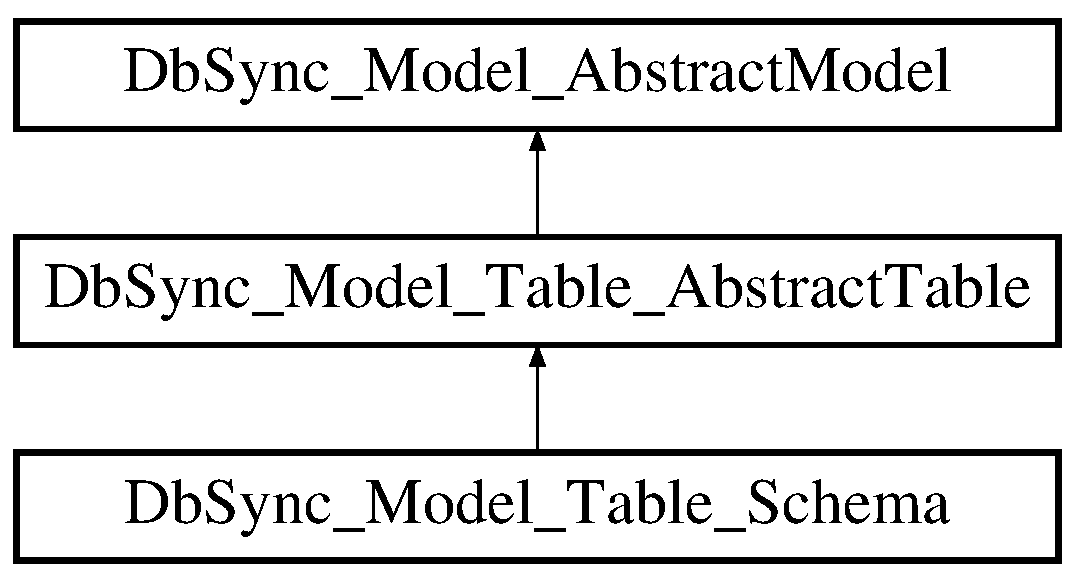
\includegraphics[height=3.000000cm]{classDbSync__Model__Table__Schema}
\end{center}
\end{figure}
\subsection*{Public Member Functions}
\begin{DoxyCompactItemize}
\item 
\hyperlink{classDbSync__Model__Table__Schema_a586a5bb7a85ccb3c591da8a67a5dda11}{generateConfigData} ()
\item 
\hyperlink{classDbSync__Model__Table__Schema_aeeedfe22d6bf19c207e788ba04f94eec}{generateSql} ()
\item 
\hyperlink{classDbSync__Model__Table__Schema_a4224bbc20523b954a9503f3c57d8e0b6}{dropDbTable} ()
\end{DoxyCompactItemize}


\subsection{Member Function Documentation}
\hypertarget{classDbSync__Model__Table__Schema_a4224bbc20523b954a9503f3c57d8e0b6}{
\index{DbSync\_\-Model\_\-Table\_\-Schema@{DbSync\_\-Model\_\-Table\_\-Schema}!dropDbTable@{dropDbTable}}
\index{dropDbTable@{dropDbTable}!DbSync_Model_Table_Schema@{DbSync\_\-Model\_\-Table\_\-Schema}}
\subsubsection[{dropDbTable}]{\setlength{\rightskip}{0pt plus 5cm}DbSync\_\-Model\_\-Table\_\-Schema::dropDbTable (
\begin{DoxyParamCaption}
{}
\end{DoxyParamCaption}
)}}
\label{classDbSync__Model__Table__Schema_a4224bbc20523b954a9503f3c57d8e0b6}
Delete Table

\begin{DoxyReturn}{Returns}
boolen 
\end{DoxyReturn}
\hypertarget{classDbSync__Model__Table__Schema_a586a5bb7a85ccb3c591da8a67a5dda11}{
\index{DbSync\_\-Model\_\-Table\_\-Schema@{DbSync\_\-Model\_\-Table\_\-Schema}!generateConfigData@{generateConfigData}}
\index{generateConfigData@{generateConfigData}!DbSync_Model_Table_Schema@{DbSync\_\-Model\_\-Table\_\-Schema}}
\subsubsection[{generateConfigData}]{\setlength{\rightskip}{0pt plus 5cm}DbSync\_\-Model\_\-Table\_\-Schema::generateConfigData (
\begin{DoxyParamCaption}
{}
\end{DoxyParamCaption}
)}}
\label{classDbSync__Model__Table__Schema_a586a5bb7a85ccb3c591da8a67a5dda11}
Get data to store in config file

\begin{DoxyReturn}{Returns}
array 
\end{DoxyReturn}
\hypertarget{classDbSync__Model__Table__Schema_aeeedfe22d6bf19c207e788ba04f94eec}{
\index{DbSync\_\-Model\_\-Table\_\-Schema@{DbSync\_\-Model\_\-Table\_\-Schema}!generateSql@{generateSql}}
\index{generateSql@{generateSql}!DbSync_Model_Table_Schema@{DbSync\_\-Model\_\-Table\_\-Schema}}
\subsubsection[{generateSql}]{\setlength{\rightskip}{0pt plus 5cm}DbSync\_\-Model\_\-Table\_\-Schema::generateSql (
\begin{DoxyParamCaption}
{}
\end{DoxyParamCaption}
)}}
\label{classDbSync__Model__Table__Schema_aeeedfe22d6bf19c207e788ba04f94eec}
Generate Alter Table

\begin{DoxyReturn}{Returns}
string 
\end{DoxyReturn}

\begin{DoxyExceptions}{Exceptions}
{\em \hyperlink{classDbSync__Exception}{DbSync\_\-Exception}} & \\
\hline
\end{DoxyExceptions}


The documentation for this class was generated from the following file:\begin{DoxyCompactItemize}
\item 
DbSync/Model/Table/Schema.php\end{DoxyCompactItemize}

\hypertarget{classDbSync__Model__Table__Trigger}{
\section{DbSync\_\-Model\_\-Table\_\-Trigger Class Reference}
\label{classDbSync__Model__Table__Trigger}\index{DbSync\_\-Model\_\-Table\_\-Trigger@{DbSync\_\-Model\_\-Table\_\-Trigger}}
}
Inheritance diagram for DbSync\_\-Model\_\-Table\_\-Trigger:\begin{figure}[H]
\begin{center}
\leavevmode
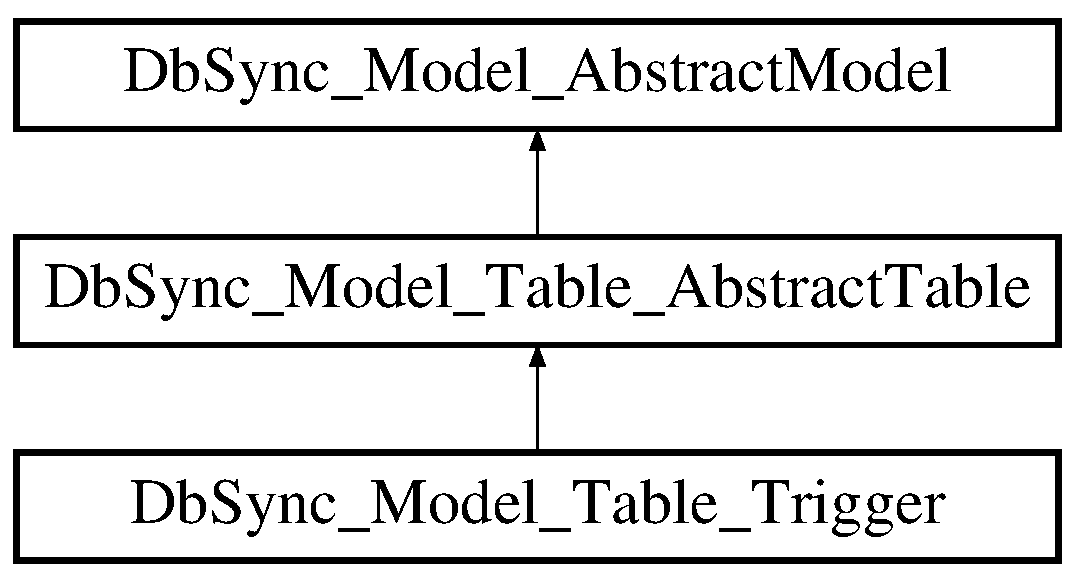
\includegraphics[height=3.000000cm]{classDbSync__Model__Table__Trigger}
\end{center}
\end{figure}
\subsection*{Public Member Functions}
\begin{DoxyCompactItemize}
\item 
\hyperlink{classDbSync__Model__Table__Trigger_a997b0c6e7fea55d82c515efabd6248e1}{getTriggerName} ()
\item 
\hyperlink{classDbSync__Model__Table__Trigger_a65fb6390628a66a3427966a012e1a90d}{setTriggerName} (\$triggerName)
\item 
\hyperlink{classDbSync__Model__Table__Trigger_a82965dc7d44b8c3722b4830c6c7cc7ea}{getName} ()
\item 
\hyperlink{classDbSync__Model__Table__Trigger_a8b13bee47b742b987a07533dba66da76}{getTableName} ()
\item 
\hyperlink{classDbSync__Model__Table__Trigger_aee02868e4b67cd7df75e7a2e1d7a354f}{generateConfigData} ()
\item 
\hyperlink{classDbSync__Model__Table__Trigger_a97d3977f816145195c174e8c460652b6}{generateSql} ()
\item 
\hyperlink{classDbSync__Model__Table__Trigger_abfa0a80448a4a9c5eb22dafe24d75697}{dropTrigger} ()
\item 
\hyperlink{classDbSync__Model__Table__Trigger_a7e5d9106415d0be267a1200851f780a5}{getListDb} (\$tables)
\item 
\hyperlink{classDbSync__Model__Table__Trigger_a90b0638071521cb7aa66eb69e651dd81}{getListConfig} (\$tables)
\item 
\hyperlink{classDbSync__Model__Table__Trigger_ae0731c9fbb1b7c293e05ca05af4ca2aa}{getList} (\$tables)
\item 
\hyperlink{classDbSync__Model__Table__Trigger_acaf99517d87453f4383ea37421ddf3b5}{hasDbTrigger} ()
\end{DoxyCompactItemize}
\subsection*{Protected Attributes}
\begin{DoxyCompactItemize}
\item 
\hypertarget{classDbSync__Model__Table__Trigger_ad715a813c905bc187ff54cf2ea23bbe4}{
{\bfseries \$\_\-triggerName}}
\label{classDbSync__Model__Table__Trigger_ad715a813c905bc187ff54cf2ea23bbe4}

\end{DoxyCompactItemize}


\subsection{Member Function Documentation}
\hypertarget{classDbSync__Model__Table__Trigger_abfa0a80448a4a9c5eb22dafe24d75697}{
\index{DbSync\_\-Model\_\-Table\_\-Trigger@{DbSync\_\-Model\_\-Table\_\-Trigger}!dropTrigger@{dropTrigger}}
\index{dropTrigger@{dropTrigger}!DbSync_Model_Table_Trigger@{DbSync\_\-Model\_\-Table\_\-Trigger}}
\subsubsection[{dropTrigger}]{\setlength{\rightskip}{0pt plus 5cm}DbSync\_\-Model\_\-Table\_\-Trigger::dropTrigger (
\begin{DoxyParamCaption}
{}
\end{DoxyParamCaption}
)}}
\label{classDbSync__Model__Table__Trigger_abfa0a80448a4a9c5eb22dafe24d75697}
Delete Table

\begin{DoxyReturn}{Returns}
boolen 
\end{DoxyReturn}
\hypertarget{classDbSync__Model__Table__Trigger_aee02868e4b67cd7df75e7a2e1d7a354f}{
\index{DbSync\_\-Model\_\-Table\_\-Trigger@{DbSync\_\-Model\_\-Table\_\-Trigger}!generateConfigData@{generateConfigData}}
\index{generateConfigData@{generateConfigData}!DbSync_Model_Table_Trigger@{DbSync\_\-Model\_\-Table\_\-Trigger}}
\subsubsection[{generateConfigData}]{\setlength{\rightskip}{0pt plus 5cm}DbSync\_\-Model\_\-Table\_\-Trigger::generateConfigData (
\begin{DoxyParamCaption}
{}
\end{DoxyParamCaption}
)}}
\label{classDbSync__Model__Table__Trigger_aee02868e4b67cd7df75e7a2e1d7a354f}
Get data to store in config file

\begin{DoxyReturn}{Returns}
array 
\end{DoxyReturn}
\hypertarget{classDbSync__Model__Table__Trigger_a97d3977f816145195c174e8c460652b6}{
\index{DbSync\_\-Model\_\-Table\_\-Trigger@{DbSync\_\-Model\_\-Table\_\-Trigger}!generateSql@{generateSql}}
\index{generateSql@{generateSql}!DbSync_Model_Table_Trigger@{DbSync\_\-Model\_\-Table\_\-Trigger}}
\subsubsection[{generateSql}]{\setlength{\rightskip}{0pt plus 5cm}DbSync\_\-Model\_\-Table\_\-Trigger::generateSql (
\begin{DoxyParamCaption}
{}
\end{DoxyParamCaption}
)}}
\label{classDbSync__Model__Table__Trigger_a97d3977f816145195c174e8c460652b6}
Generate Sql code

\begin{DoxyReturn}{Returns}
string 
\end{DoxyReturn}

\begin{DoxyExceptions}{Exceptions}
{\em \hyperlink{classDbSync__Exception}{DbSync\_\-Exception}} & \\
\hline
\end{DoxyExceptions}
\hypertarget{classDbSync__Model__Table__Trigger_ae0731c9fbb1b7c293e05ca05af4ca2aa}{
\index{DbSync\_\-Model\_\-Table\_\-Trigger@{DbSync\_\-Model\_\-Table\_\-Trigger}!getList@{getList}}
\index{getList@{getList}!DbSync_Model_Table_Trigger@{DbSync\_\-Model\_\-Table\_\-Trigger}}
\subsubsection[{getList}]{\setlength{\rightskip}{0pt plus 5cm}DbSync\_\-Model\_\-Table\_\-Trigger::getList (
\begin{DoxyParamCaption}
\item[{\$}]{tables}
\end{DoxyParamCaption}
)}}
\label{classDbSync__Model__Table__Trigger_ae0731c9fbb1b7c293e05ca05af4ca2aa}
Get db tables list


\begin{DoxyParams}[1]{Parameters}
array & {\em \$tables} & \\
\hline
\end{DoxyParams}
\begin{DoxyReturn}{Returns}
array 
\end{DoxyReturn}
\hypertarget{classDbSync__Model__Table__Trigger_a90b0638071521cb7aa66eb69e651dd81}{
\index{DbSync\_\-Model\_\-Table\_\-Trigger@{DbSync\_\-Model\_\-Table\_\-Trigger}!getListConfig@{getListConfig}}
\index{getListConfig@{getListConfig}!DbSync_Model_Table_Trigger@{DbSync\_\-Model\_\-Table\_\-Trigger}}
\subsubsection[{getListConfig}]{\setlength{\rightskip}{0pt plus 5cm}DbSync\_\-Model\_\-Table\_\-Trigger::getListConfig (
\begin{DoxyParamCaption}
\item[{\$}]{tables}
\end{DoxyParamCaption}
)}}
\label{classDbSync__Model__Table__Trigger_a90b0638071521cb7aa66eb69e651dd81}
Get data tables list


\begin{DoxyParams}[1]{Parameters}
array & {\em \$tables} & \\
\hline
\end{DoxyParams}
\begin{DoxyReturn}{Returns}
array 
\end{DoxyReturn}
\hypertarget{classDbSync__Model__Table__Trigger_a7e5d9106415d0be267a1200851f780a5}{
\index{DbSync\_\-Model\_\-Table\_\-Trigger@{DbSync\_\-Model\_\-Table\_\-Trigger}!getListDb@{getListDb}}
\index{getListDb@{getListDb}!DbSync_Model_Table_Trigger@{DbSync\_\-Model\_\-Table\_\-Trigger}}
\subsubsection[{getListDb}]{\setlength{\rightskip}{0pt plus 5cm}DbSync\_\-Model\_\-Table\_\-Trigger::getListDb (
\begin{DoxyParamCaption}
\item[{\$}]{tables}
\end{DoxyParamCaption}
)}}
\label{classDbSync__Model__Table__Trigger_a7e5d9106415d0be267a1200851f780a5}
Get triggers list


\begin{DoxyParams}[1]{Parameters}
array & {\em \$tables} & \\
\hline
\end{DoxyParams}
\begin{DoxyReturn}{Returns}
array 
\end{DoxyReturn}
\hypertarget{classDbSync__Model__Table__Trigger_a82965dc7d44b8c3722b4830c6c7cc7ea}{
\index{DbSync\_\-Model\_\-Table\_\-Trigger@{DbSync\_\-Model\_\-Table\_\-Trigger}!getName@{getName}}
\index{getName@{getName}!DbSync_Model_Table_Trigger@{DbSync\_\-Model\_\-Table\_\-Trigger}}
\subsubsection[{getName}]{\setlength{\rightskip}{0pt plus 5cm}DbSync\_\-Model\_\-Table\_\-Trigger::getName (
\begin{DoxyParamCaption}
{}
\end{DoxyParamCaption}
)}}
\label{classDbSync__Model__Table__Trigger_a82965dc7d44b8c3722b4830c6c7cc7ea}
Get trigger name

\begin{DoxyReturn}{Returns}
string 
\end{DoxyReturn}


Reimplemented from \hyperlink{classDbSync__Model__Table__AbstractTable_a88726b043a43248114ca3e3faa9025d2}{DbSync\_\-Model\_\-Table\_\-AbstractTable}.

\hypertarget{classDbSync__Model__Table__Trigger_a8b13bee47b742b987a07533dba66da76}{
\index{DbSync\_\-Model\_\-Table\_\-Trigger@{DbSync\_\-Model\_\-Table\_\-Trigger}!getTableName@{getTableName}}
\index{getTableName@{getTableName}!DbSync_Model_Table_Trigger@{DbSync\_\-Model\_\-Table\_\-Trigger}}
\subsubsection[{getTableName}]{\setlength{\rightskip}{0pt plus 5cm}DbSync\_\-Model\_\-Table\_\-Trigger::getTableName (
\begin{DoxyParamCaption}
{}
\end{DoxyParamCaption}
)}}
\label{classDbSync__Model__Table__Trigger_a8b13bee47b742b987a07533dba66da76}
Get table name

\begin{DoxyReturn}{Returns}
string 
\end{DoxyReturn}


Reimplemented from \hyperlink{classDbSync__Model__Table__AbstractTable_a8ee4b6ffc0539b45a791bc04eebe7548}{DbSync\_\-Model\_\-Table\_\-AbstractTable}.

\hypertarget{classDbSync__Model__Table__Trigger_a997b0c6e7fea55d82c515efabd6248e1}{
\index{DbSync\_\-Model\_\-Table\_\-Trigger@{DbSync\_\-Model\_\-Table\_\-Trigger}!getTriggerName@{getTriggerName}}
\index{getTriggerName@{getTriggerName}!DbSync_Model_Table_Trigger@{DbSync\_\-Model\_\-Table\_\-Trigger}}
\subsubsection[{getTriggerName}]{\setlength{\rightskip}{0pt plus 5cm}DbSync\_\-Model\_\-Table\_\-Trigger::getTriggerName (
\begin{DoxyParamCaption}
{}
\end{DoxyParamCaption}
)}}
\label{classDbSync__Model__Table__Trigger_a997b0c6e7fea55d82c515efabd6248e1}
Get trigger name

\begin{DoxyReturn}{Returns}
string 
\end{DoxyReturn}

\begin{DoxyExceptions}{Exceptions}
{\em \hyperlink{classDbSync__Exception}{DbSync\_\-Exception}} & \\
\hline
\end{DoxyExceptions}
\hypertarget{classDbSync__Model__Table__Trigger_acaf99517d87453f4383ea37421ddf3b5}{
\index{DbSync\_\-Model\_\-Table\_\-Trigger@{DbSync\_\-Model\_\-Table\_\-Trigger}!hasDbTrigger@{hasDbTrigger}}
\index{hasDbTrigger@{hasDbTrigger}!DbSync_Model_Table_Trigger@{DbSync\_\-Model\_\-Table\_\-Trigger}}
\subsubsection[{hasDbTrigger}]{\setlength{\rightskip}{0pt plus 5cm}DbSync\_\-Model\_\-Table\_\-Trigger::hasDbTrigger (
\begin{DoxyParamCaption}
{}
\end{DoxyParamCaption}
)}}
\label{classDbSync__Model__Table__Trigger_acaf99517d87453f4383ea37421ddf3b5}
Is db table exists

\begin{DoxyReturn}{Returns}
boolen 
\end{DoxyReturn}
\hypertarget{classDbSync__Model__Table__Trigger_a65fb6390628a66a3427966a012e1a90d}{
\index{DbSync\_\-Model\_\-Table\_\-Trigger@{DbSync\_\-Model\_\-Table\_\-Trigger}!setTriggerName@{setTriggerName}}
\index{setTriggerName@{setTriggerName}!DbSync_Model_Table_Trigger@{DbSync\_\-Model\_\-Table\_\-Trigger}}
\subsubsection[{setTriggerName}]{\setlength{\rightskip}{0pt plus 5cm}DbSync\_\-Model\_\-Table\_\-Trigger::setTriggerName (
\begin{DoxyParamCaption}
\item[{\$}]{triggerName}
\end{DoxyParamCaption}
)}}
\label{classDbSync__Model__Table__Trigger_a65fb6390628a66a3427966a012e1a90d}
Set trigger name


\begin{DoxyParams}[1]{Parameters}
string & {\em \$triggerName} & \\
\hline
\end{DoxyParams}
\begin{DoxyReturn}{Returns}
\hyperlink{classDbSync__Model__Table__Trigger}{DbSync\_\-Model\_\-Table\_\-Trigger} 
\end{DoxyReturn}


The documentation for this class was generated from the following file:\begin{DoxyCompactItemize}
\item 
DbSync/Model/Table/Trigger.php\end{DoxyCompactItemize}

\printindex
\end{document}
